\chapter{Background Estimation and Systematic Uncertainties}
\label{bkgEstimation}
\section{Alpha Method}
So far we presented distributions of the background based on Monte Carlo (MC) simulations. An alternative data-driven method to estimate the background is preferred because it gets rid of some systematic uncertainties that can make the simulation rather inaccurate. For instance, theoretical uncertainties on the cross section of the background processes can be avoided by applying a normalization based on data. Another example would be the systematic uncertainties related to mismodeling of the process of parton showering and hadronization of the final state quarks. Simulation of the interaction of the particles from the collision with the sensitive volumes of the detector and the readout electronics introduce yet another source of uncertainties. 

The data-driven method itself may bring other sources of uncertainties that can be as large as the theoretical uncertainties we want to avoid. Therefore, background estimation techniques cover a broad field of research beyond the material presented in this section. Here, we limit the discussion to one particular technique known as the alpha method \cite{Mozer:2016wzi}.  

For the estimation of the background in the signal region ($65 < \mj < 105$ GeV), we use the following inputs:
\begin{compact_itemize}
\item Real data distribution of $\mZV$ in control region: ($20 < \mj < 65$ GeV)  $\cup$ ($135 < \mj <220$ GeV) , which we will call $f(\mZV)^{\textrm{DATA}}_{\textrm{CR}}$
\item Simulated distribution of the dominant background (Z+jets) in  both control region and in the signal region, which we will call $f(\mZV)^{\textrm{Z+jets}}_{\textrm{CR}}$ and $f(\mZV)^{\textrm{Z+jets}}_{\textrm{SR}}$ respectively.
\item Simulated distribution of the subdominant background (VV and $t\bar{t}$) in  both control region and in the signal region, which we will call $f(\mZV)^{\textrm{sub}}_{\textrm{CR}}$ and $f(\mZV)^{\textrm{sub}}_{\textrm{SR}}$ respectively.
\end{compact_itemize}

The alpha method is applied for the dominant background of our search, which is Z+jets; for the subdominant background we use directly the MC estimation. The method exploits the correlation between the jet mass $\mj$ and the invariant mass $\mZV$, by defining a transfer factor as follows:
%%%
\begin{equation}
\alpha(\mZV) = \frac{f(\mZV)^{\textrm{Z+jets}}_{\textrm{SR}}}{f(\mZV)^{\textrm{Z+jets}}_{\textrm{CR}}}\,.
\end{equation}
%%%

The dominant background estimation in the signal region is obtained by applying that transfer factor to a pure Z+jets real data sample in the control region, i.e.:
%%%
\begin{equation}
\left \langle f(\mZV)^{\textrm{Z+jets}}_{\textrm{SR}} \right \rangle = \alpha(\mZV)
\times
\left \langle f(\mZV)^{\textrm{Z+jets}}_{\textrm{CR}} \right \rangle
\end{equation}
%%%
where the angled brackets represent a data estimation of the Z+jets background. Now the problem has to do with the estimation of the Z+jets background in the control region. Since that region is essentially signal-free, it is safe to approximate
%%%
\begin{equation}
\left \langle f(\mZV)^{\textrm{Z+jets}}_{\textrm{CR}} \right \rangle =
f(\mZV)^{\textrm{data}}_{\textrm{CR}} - f(\mZV)^{\textrm{sub}}_{\textrm{CR}}
\end{equation}
%%%
whereas the data estimation in the signal region can then be written as
\begin{equation}
\left \langle f(\mZV)^{\textrm{Z+jets}}_{\textrm{SR}} \right \rangle
=
\frac{f(\mZV)^{\textrm{Z+jets}}_{\textrm{SR}}}{f(\mZV)^{\textrm{Z+jets}}_{\textrm{CR}}}
\times
\left (
f(\mZV)^{\textrm{data}}_{\textrm{CR}} - f(\mZV)^{\textrm{sub}}_{\textrm{CR}}
\right )\,.
\label{eq:domSR}
\end{equation}

In plain words, $\alpha(\mZV)$ is the ratio of the $\mZV$ distribution in the signal region over the distribution in the control region for the dominant background, and it is shown in Fig.~\ref{fig:alpha_MVZ}. This transfer factor is then used, after controlling the presence of the subdominant backgrounds, to correct the $\mZV$ distribution in the control region that is shown in Fig.~\ref{fig:control_MVZ}. The resulting prediction in the signal region will be presented in the next section containing the unblind results. We note that the method leads to a prediction of both the shape and normalization of the dominant background in the signal region; however, we discarded the latter and retain only the shape prediction. For the estimation of the normalization, a more robust method is applied as we will explain in a moment.

In Eq.~\ref{eq:domSR}, the function $f(\mZV)$ can be modeled by a leveled exponential defined below:
\begin{equation}
f(\mZV) = \exp \left (
\frac{-\mZV}
{a(\mj) + b(\mj)\,\mZV}
\right )\,,
\end{equation}
where $a(\mj), b(\mj)$ are parameters that implicitly depend on $\mj$. In practice, we assume that these parameters are constant within a given region, i.e. there is a set of constant parameters $a^{\textrm{(SR)}}$, $b^{\textrm{(SR)}}$ that leads to a good description of the $\mZV$ distribution in the signal region, and analogously for the control region. 

Our implementation of the alpha method was coded in ROOT \cite{Antcheva:2011zz} enhanced with the RooFit extension \cite{Verkerke:2003ir}. The algorithm starts with the declaration of the probability density functions (PDF), specifically 5 leveled exponentials for the following cases:
\begin{compact_itemize}
\item Simulated dominant background in the signal region;
\item Simulated subdominant background in the signal region;
\item Simulated dominant background in the control region;
\item Simulated subdominant background in the control region;
\item Real data in the control region.
\end{compact_itemize}
In total there are 10 correlated parameters that need to be fit. The routine performs a simultaneous fit of the PDFs associated with the dominant background and real data, in order to get the best estimation of the parameters as well as the correlation matrix that allows the propagation of uncertainties to the final result. The modeling of the subdominant background is taken directly from simulation; to facilitate the convergence of the simultaneous fit during the alpha method, the parameters associated to the subdominant component are kept fixed.

The prediction of the background normalization in the signal region is derived by interpolating the data from the control region of the jet mass distribution. The baseline model for the shape of the jet mass was tuned in simulation, as indicated in Fig.~\ref{fig:fits_MJ}. In order to estimate the adequacy of the model, we made a data-based study on the viability of different alternatives. This translates directly to a systematic uncertainty in the normalization of the background in the signal region. Different model choices are shown in Fig.~\ref{thiagoFits}, and the estimated yield in the signal region is reported in Table \ref{tab:bkgtest} for each model. From these results we estimated a systematic uncertainty ($\Delta$) that ranges from 28\% in the EHP category to 42\% in the MHP category.

\begin{figure}[htb]
\centering
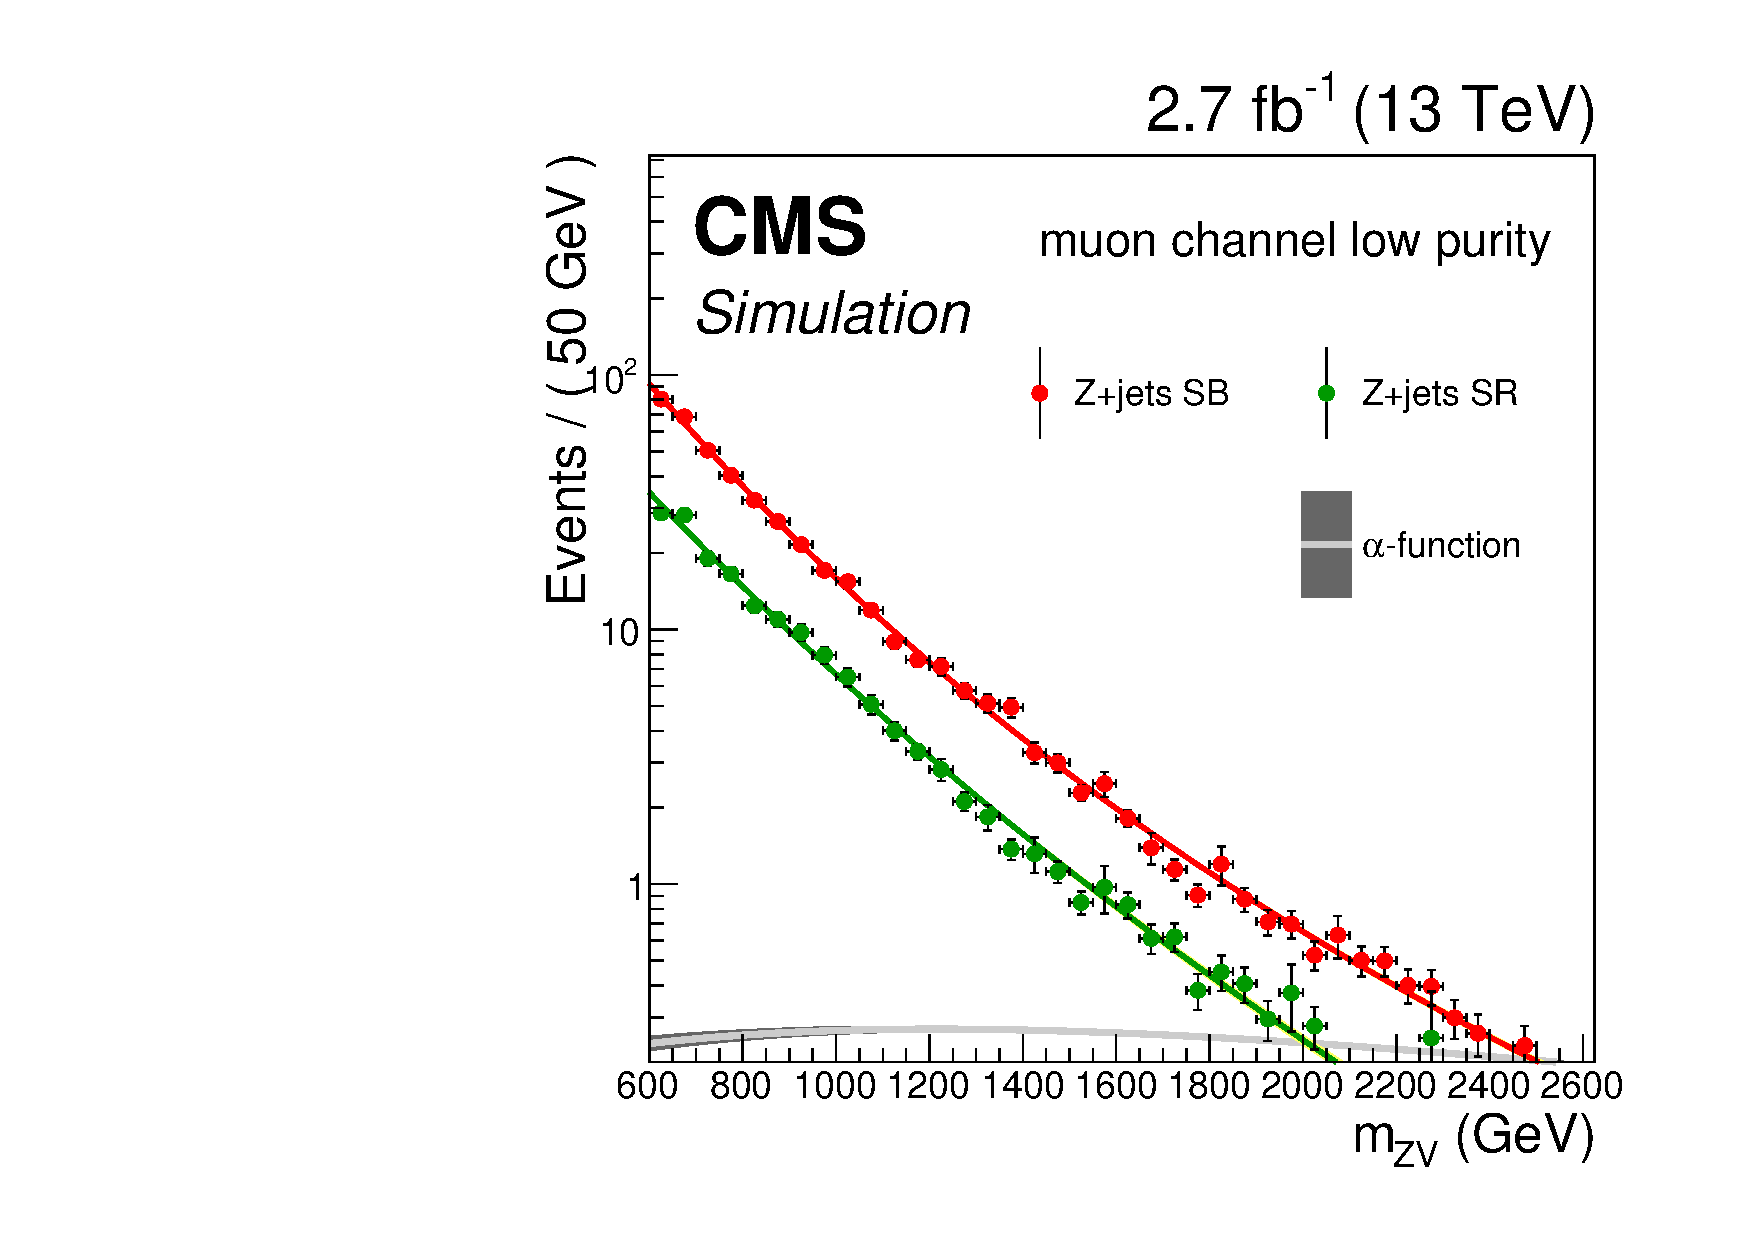
\includegraphics[width=0.47\textwidth]{figures/fits/alphaMLP.pdf}
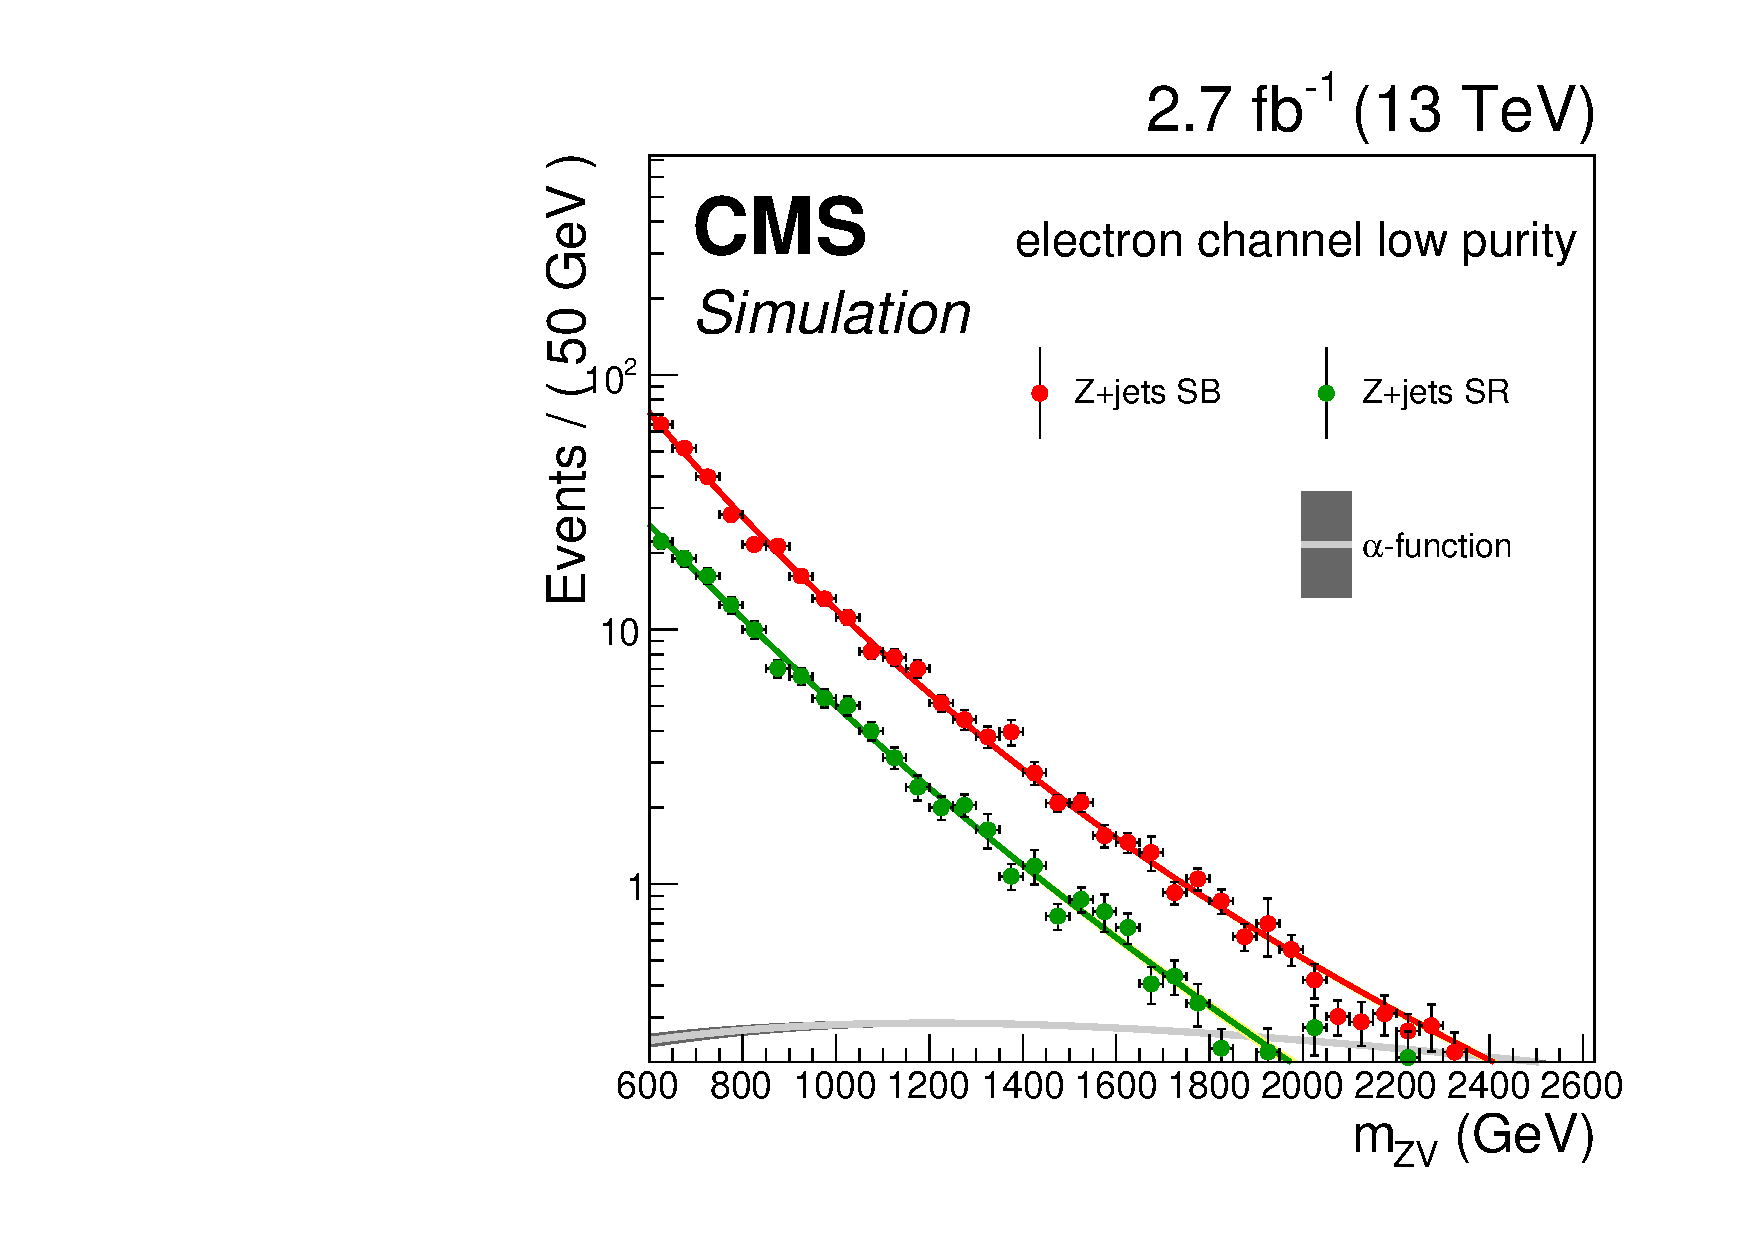
\includegraphics[width=0.47\textwidth]{figures/fits/alphaELP.pdf}\newline
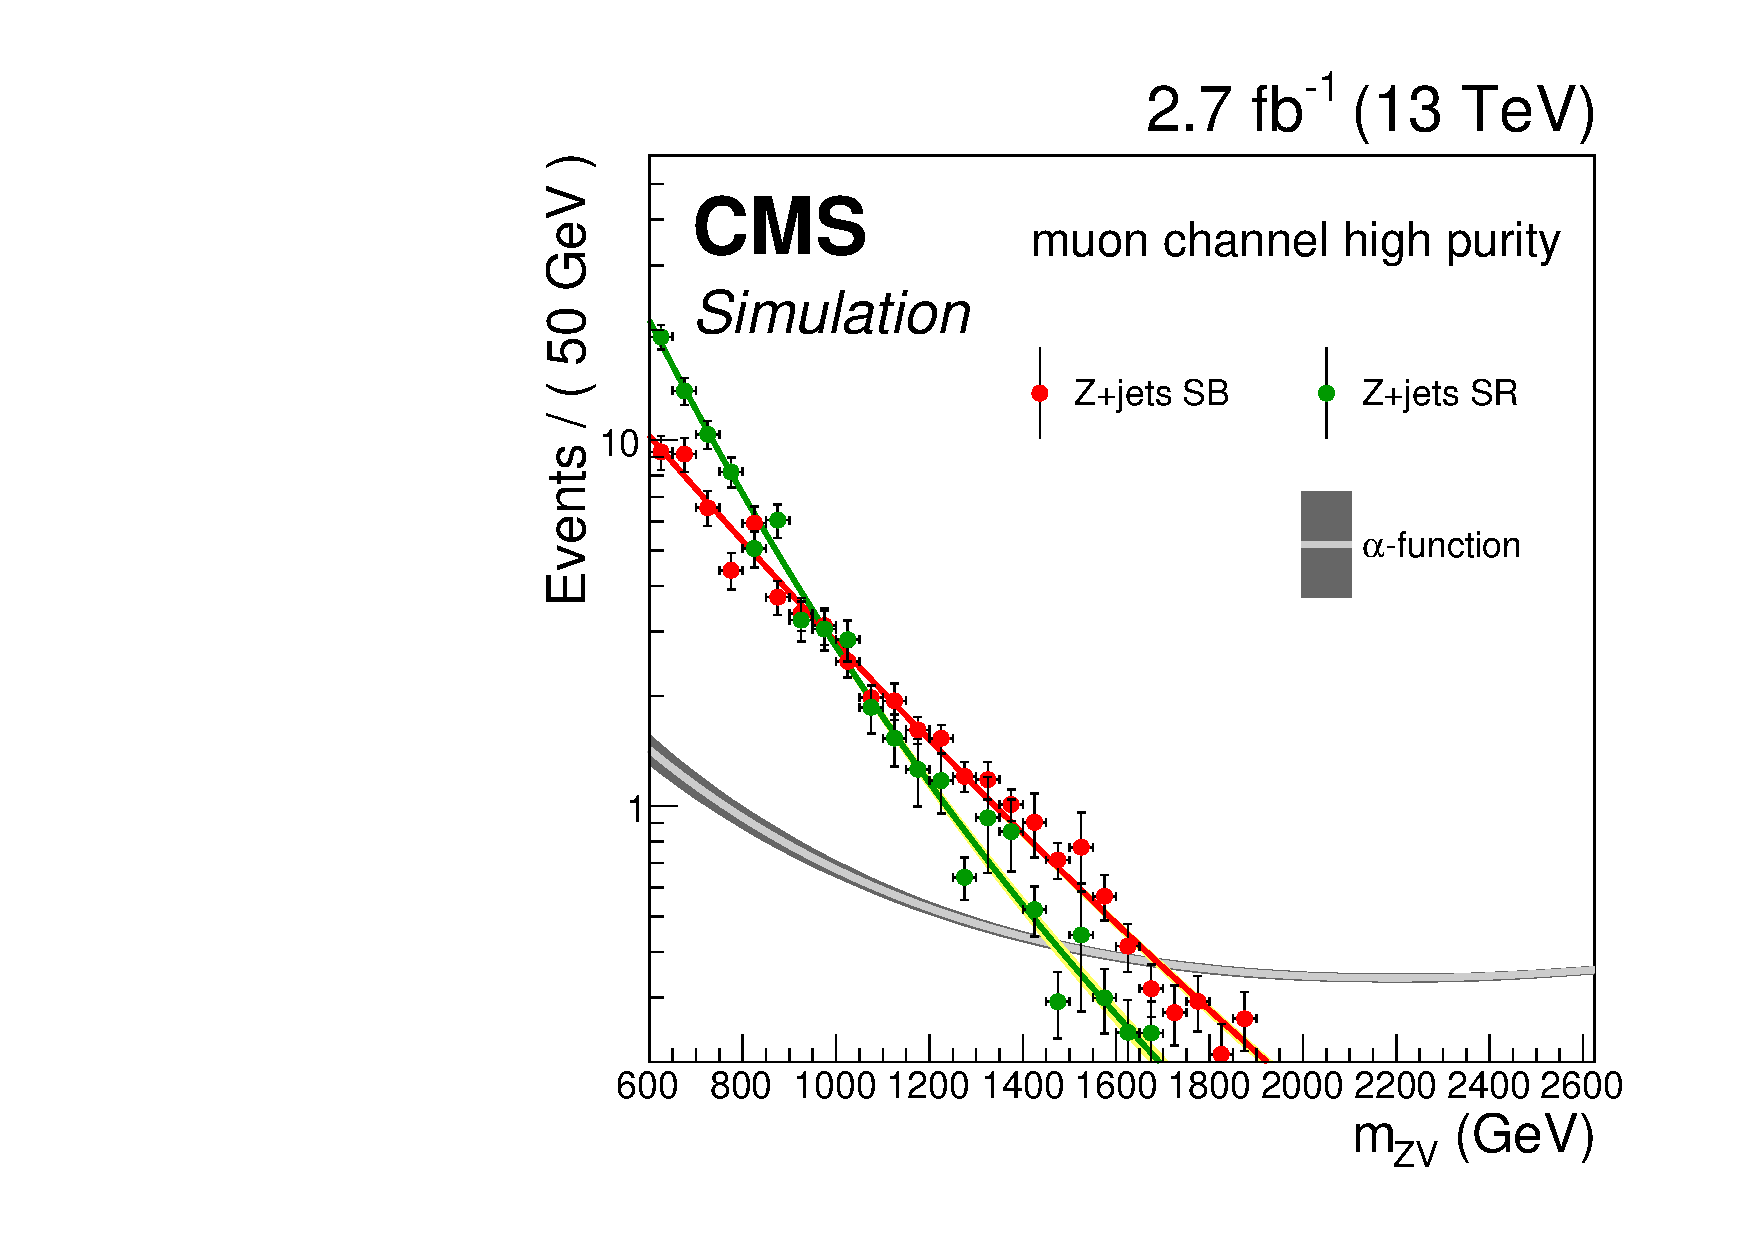
\includegraphics[width=0.47\textwidth]{figures/fits/alphaMHP.pdf}
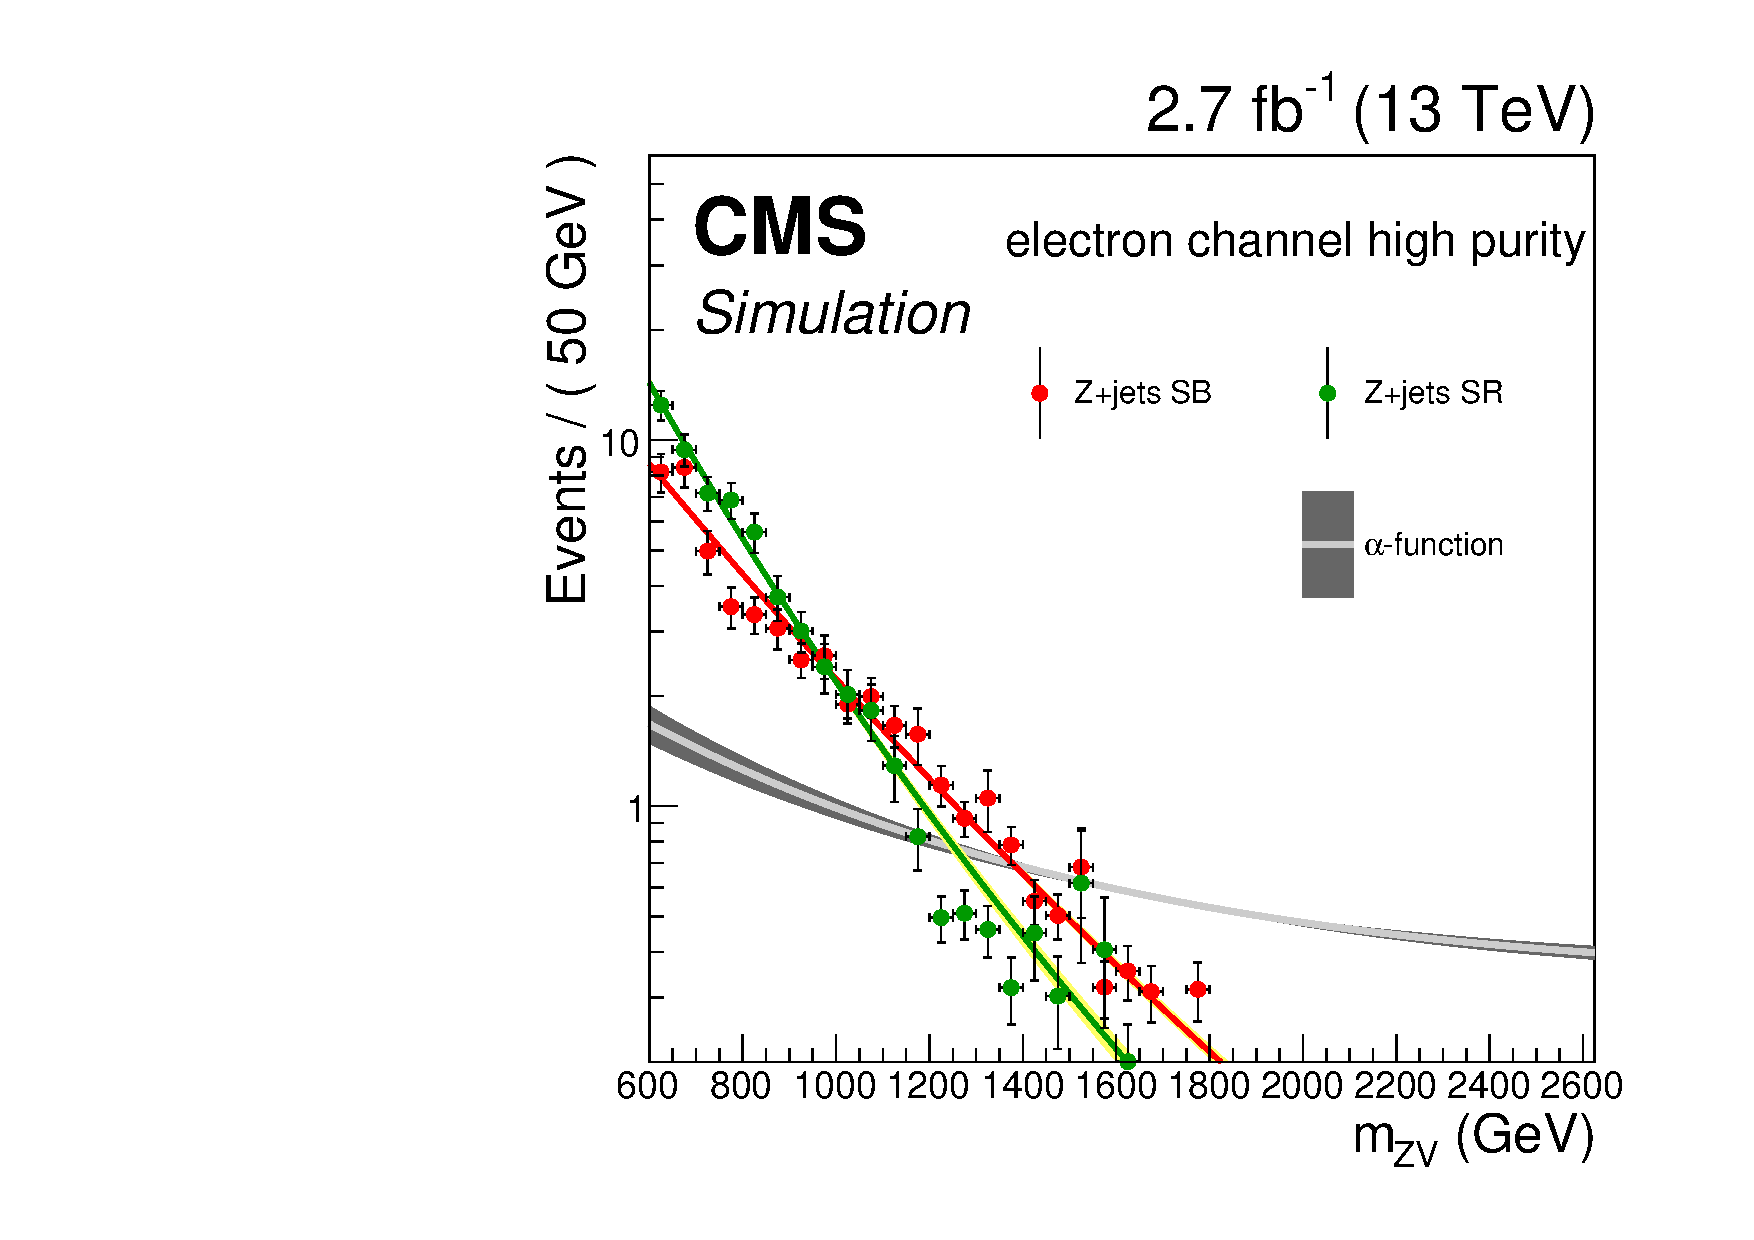
\includegraphics[width=0.47\textwidth]{figures/fits/alphaEHP.pdf}\newline
\caption[Alpha transfer factor]{
Top: $\mZV$ simulated distributions in the signal (green) and control (red) region for the low purity category,
for muons (left) and electrons (right). 
Bottom: $\mZV$ simulated distributions in the signal (green) and control (red) region for the high purity category,
for muons (left) and electrons (right). The transfer factor $\alpha(\mZV)$ is defined by the ratio ($\mZV$ signal region) / ($\mZV$ control region).
}
\label{fig:alpha_MVZ}
\end{figure}

\begin{figure}[p]
\centering
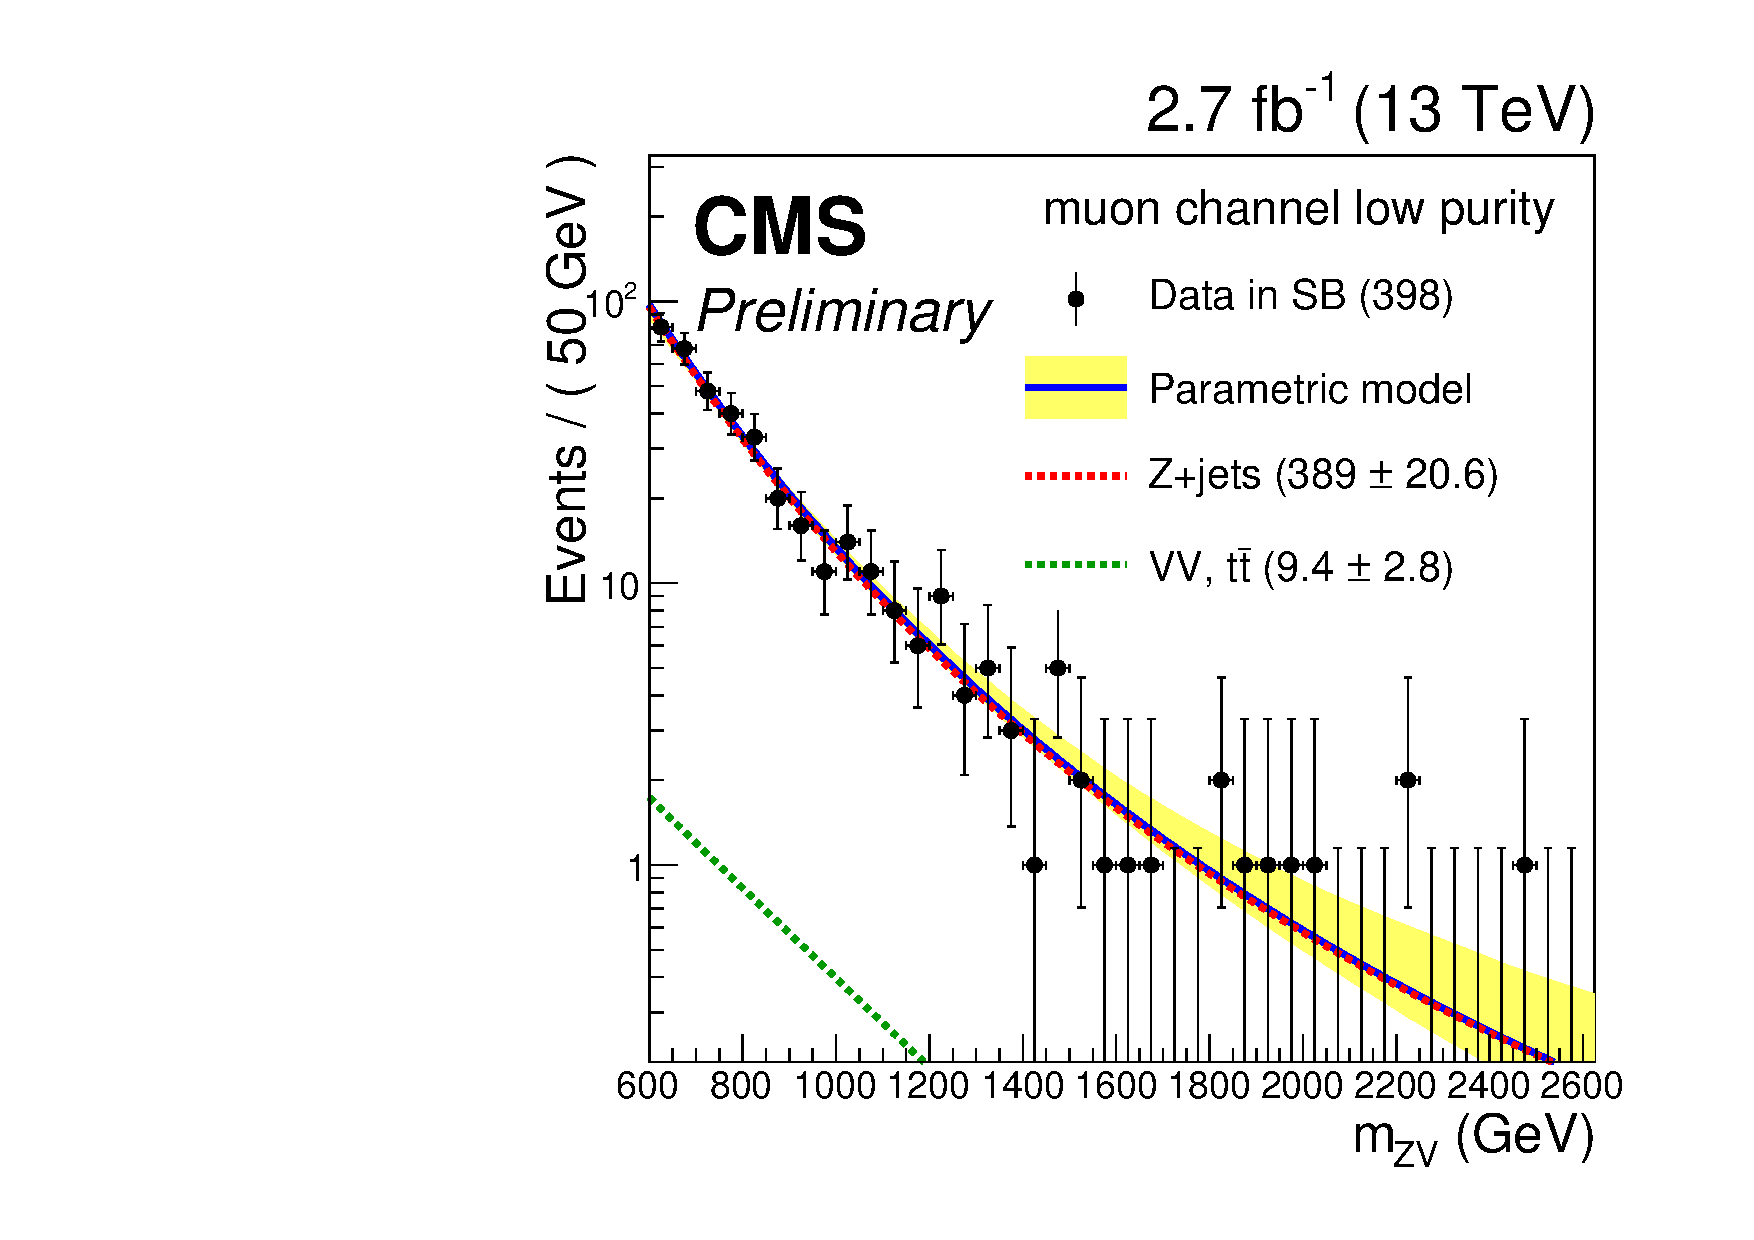
\includegraphics[width=0.47\textwidth]{figures/fits/mVZsbMLP.pdf}
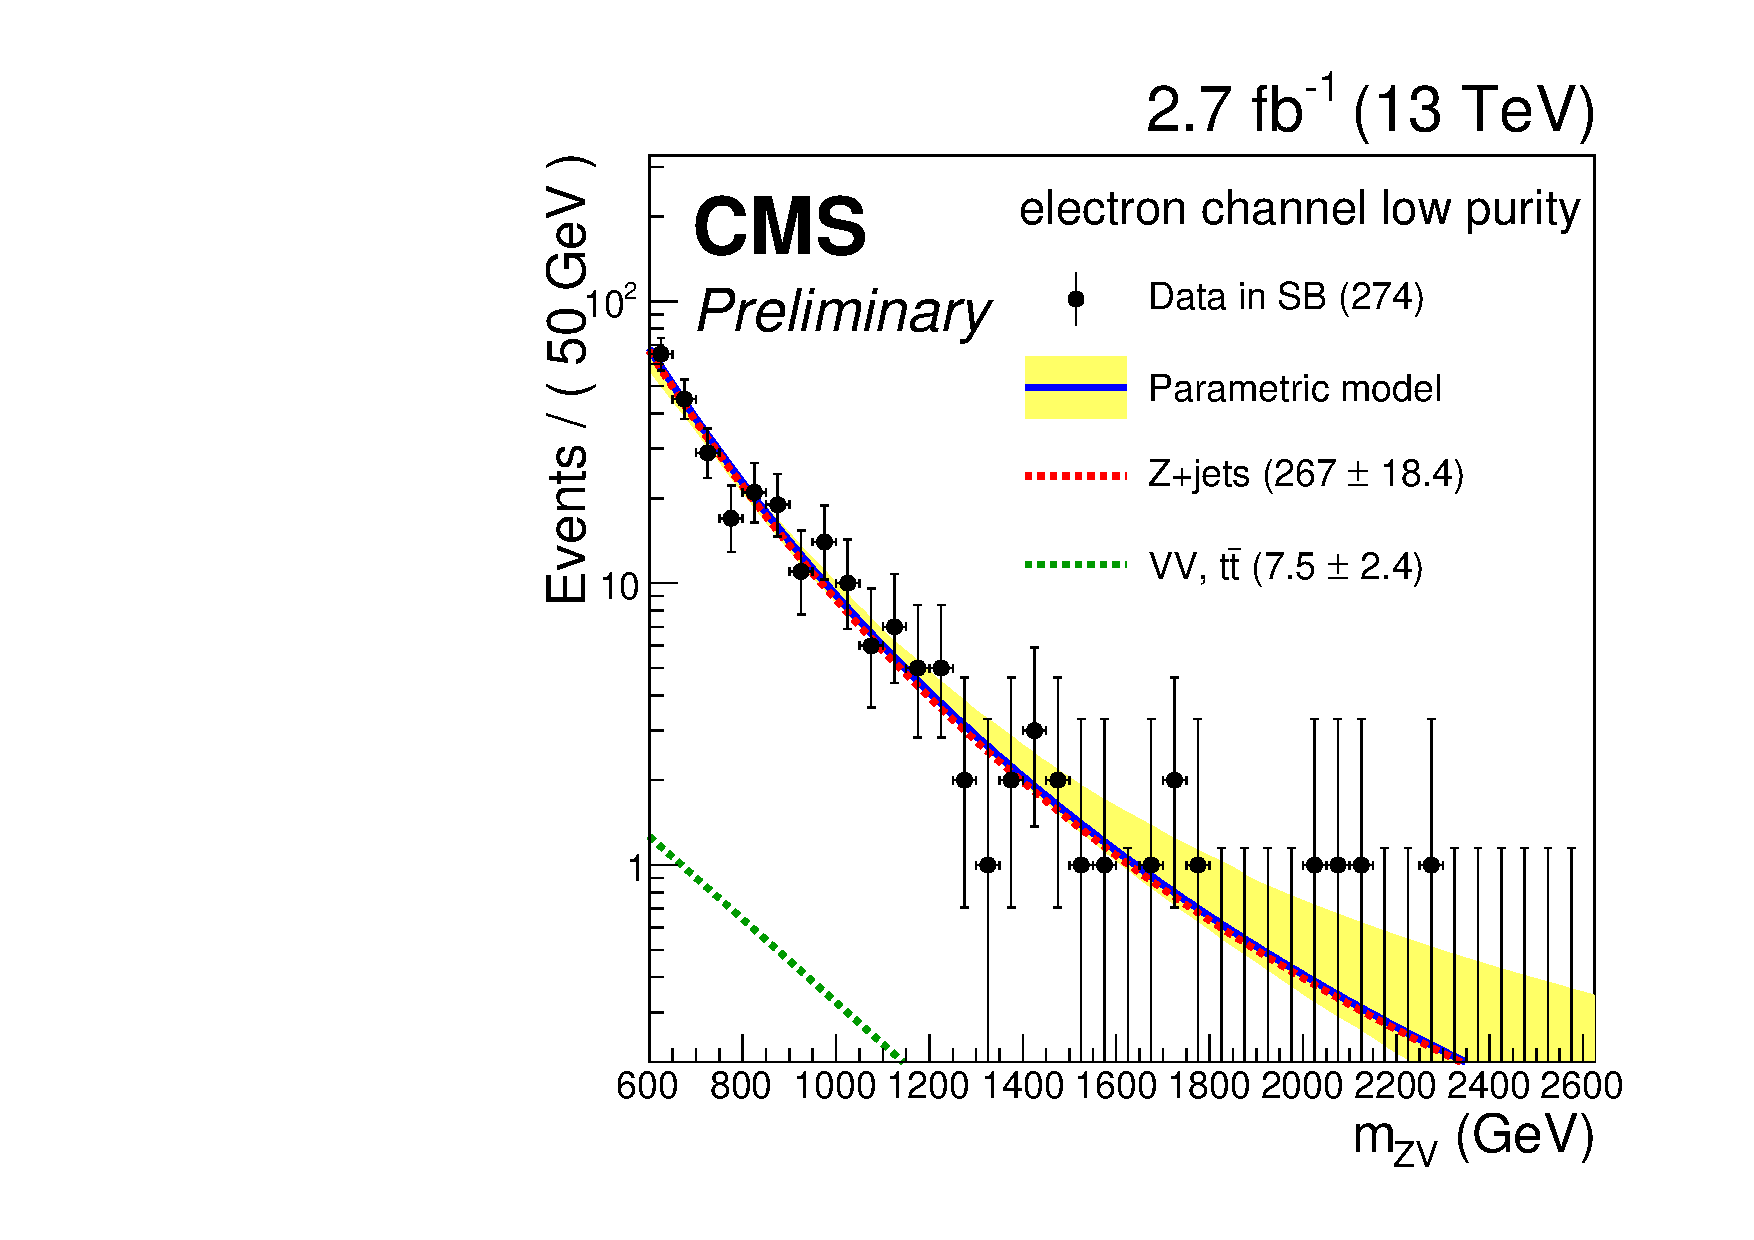
\includegraphics[width=0.47\textwidth]{figures/fits/mVZsbELP.pdf}\newline
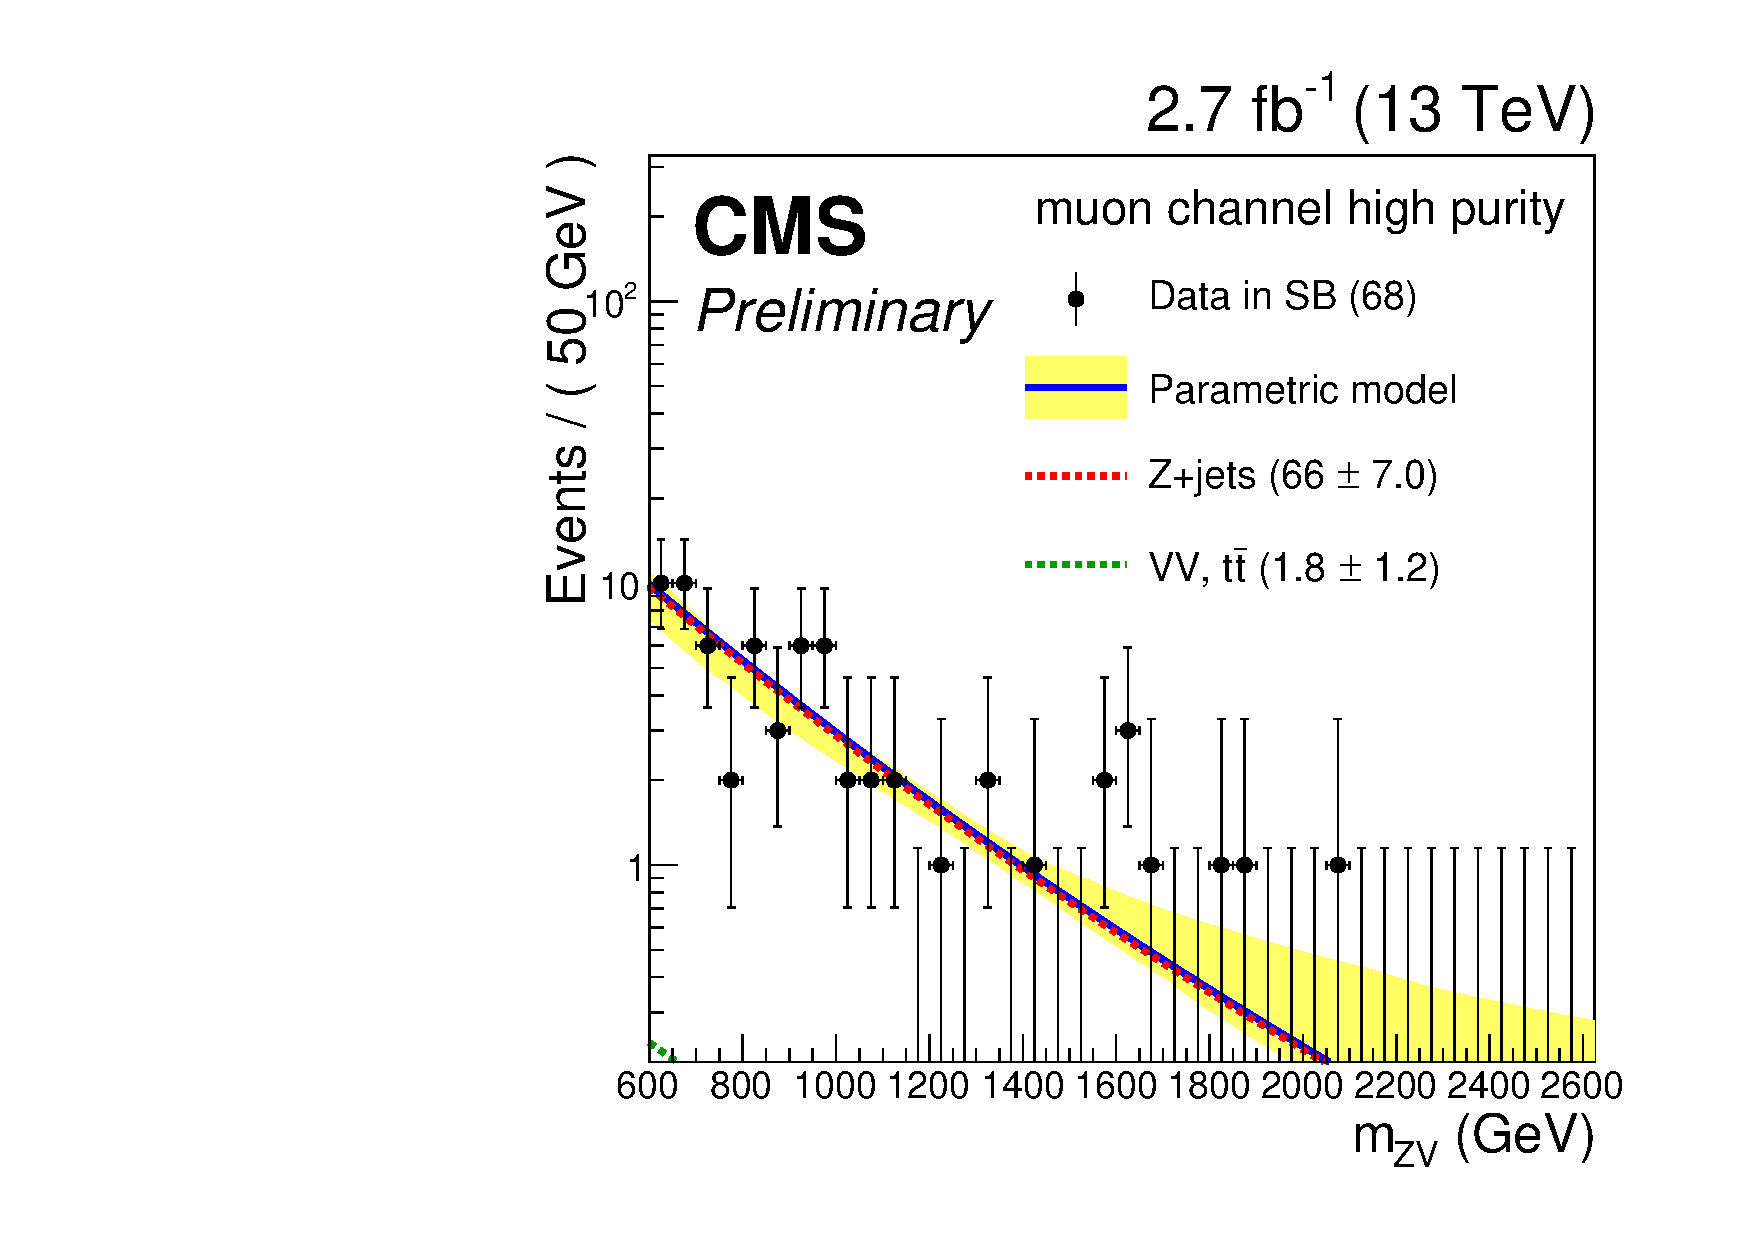
\includegraphics[width=0.47\textwidth]{figures/fits/mVZsbMHP.pdf}
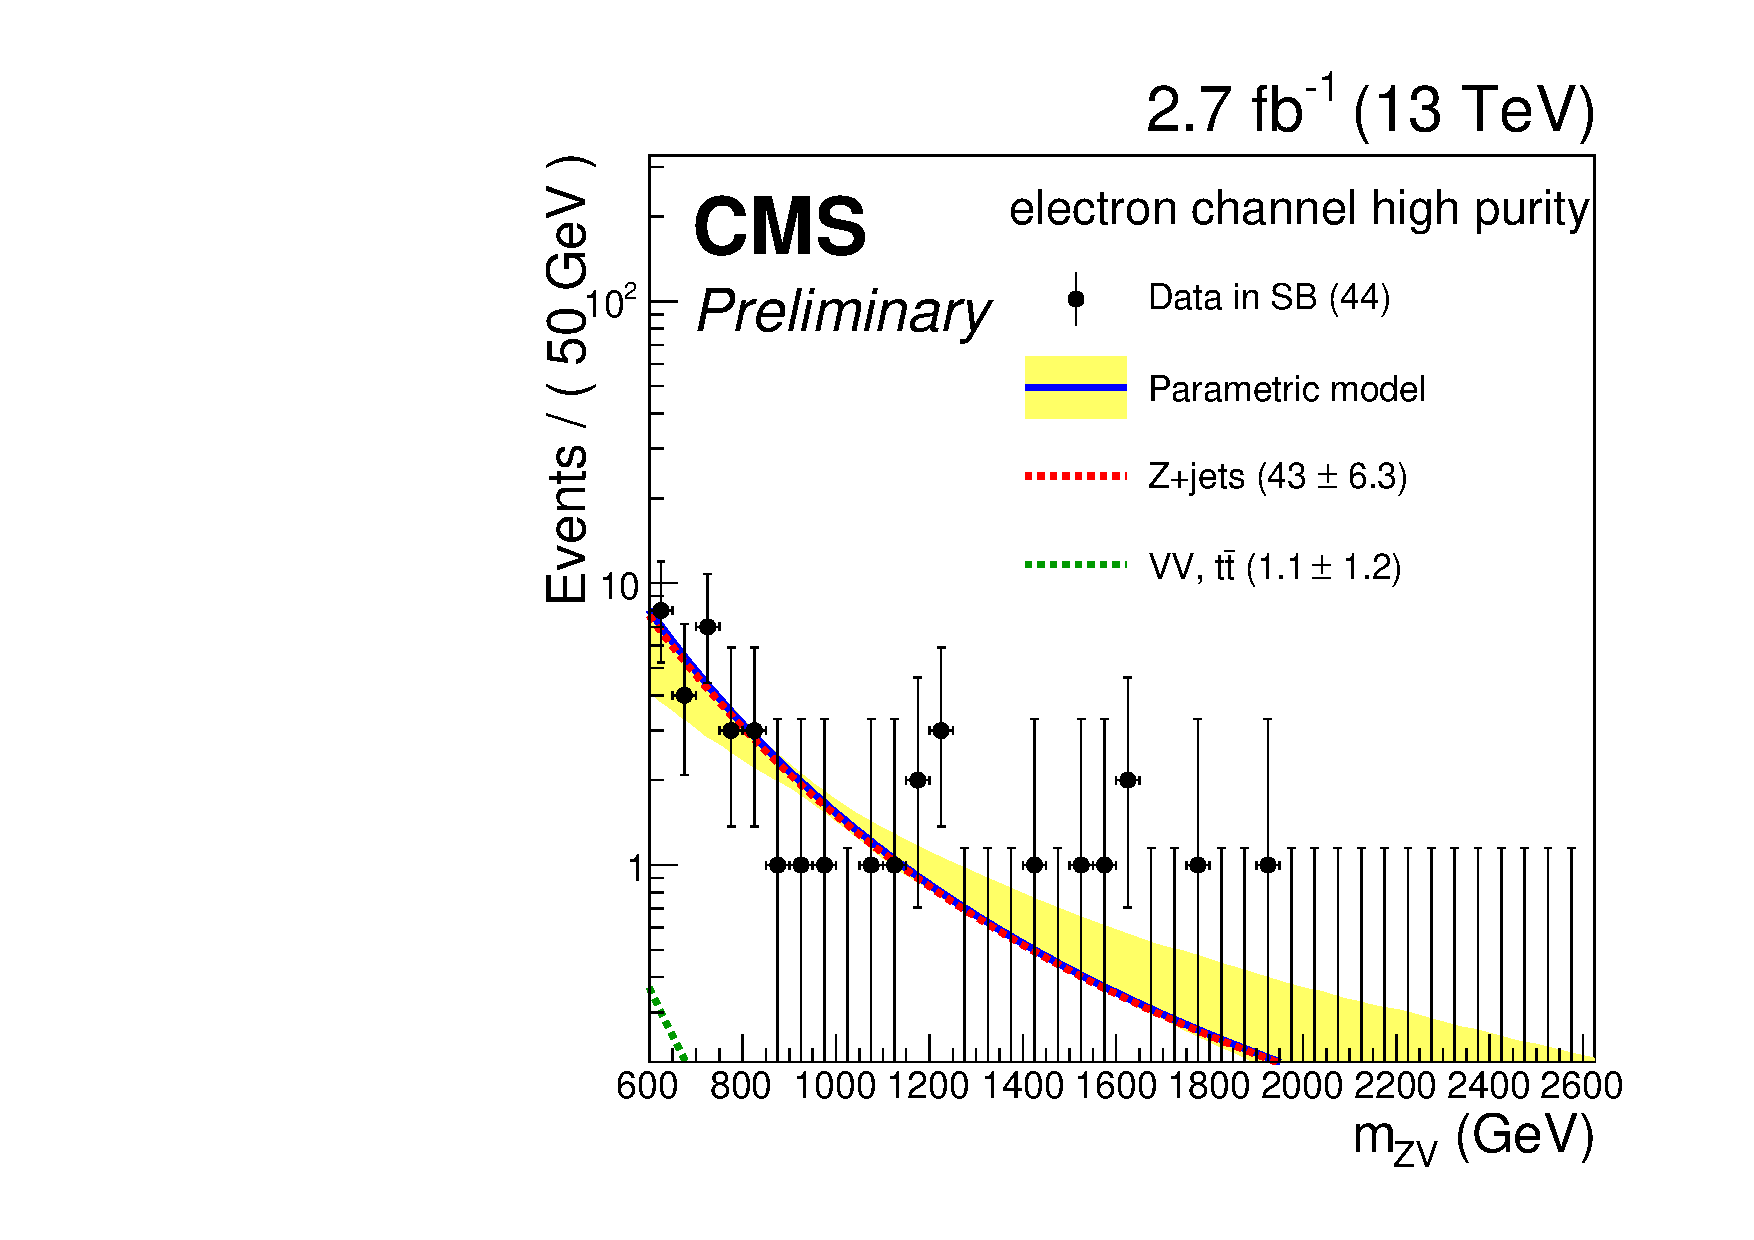
\includegraphics[width=0.47\textwidth]{figures/fits/mVZsbEHP.pdf}\newline
\caption[Invariant mass distributions in control region]{
Top: $\mZV$ distributions in the control region for the low purity category,
for muons (left) and electrons (right). 
Bottom: $\mZV$ distributions in the signal region for the high purity category,
for muons (left) and electrons (right). 
}
\label{fig:control_MVZ}
\end{figure}

\begin{figure}[p]
\centering
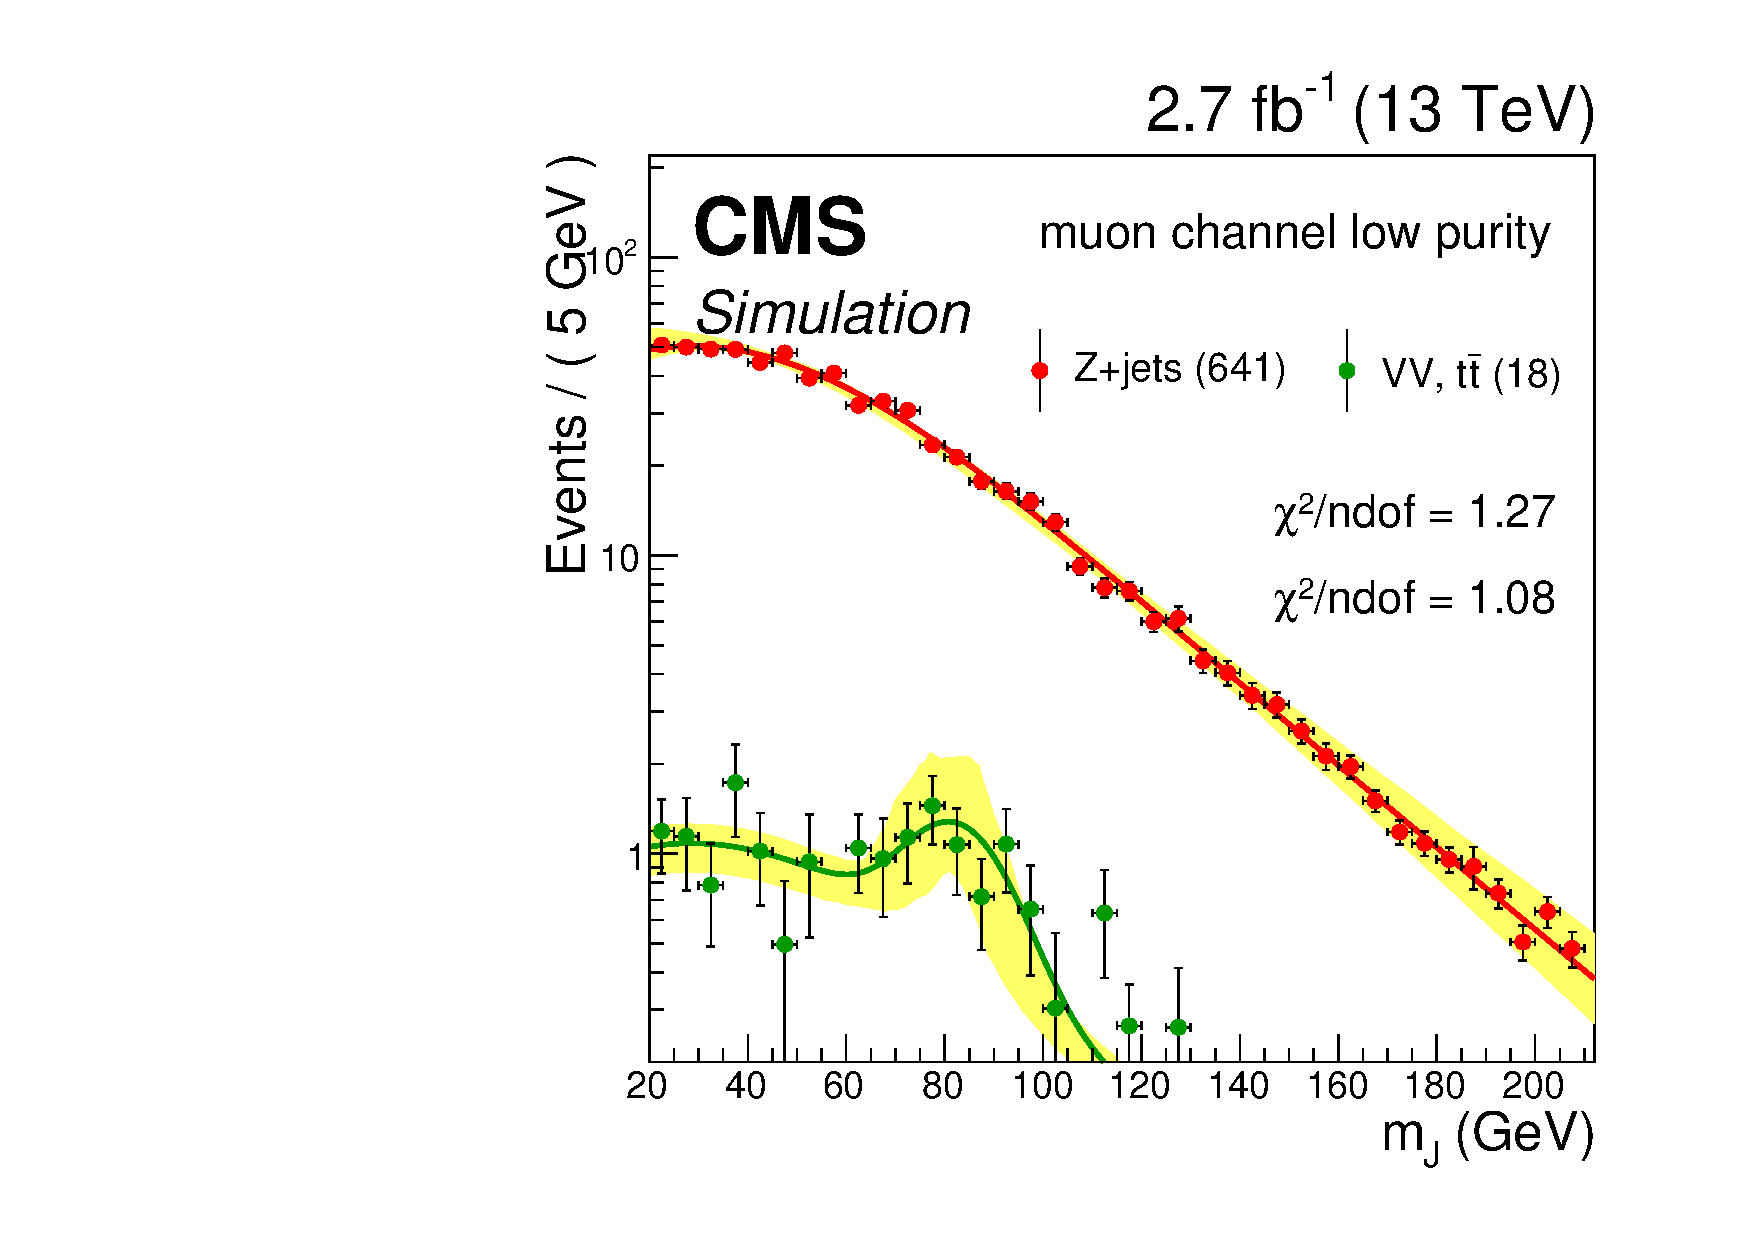
\includegraphics[width=0.47\textwidth]{figures/fits/bkgMjMLP.pdf}
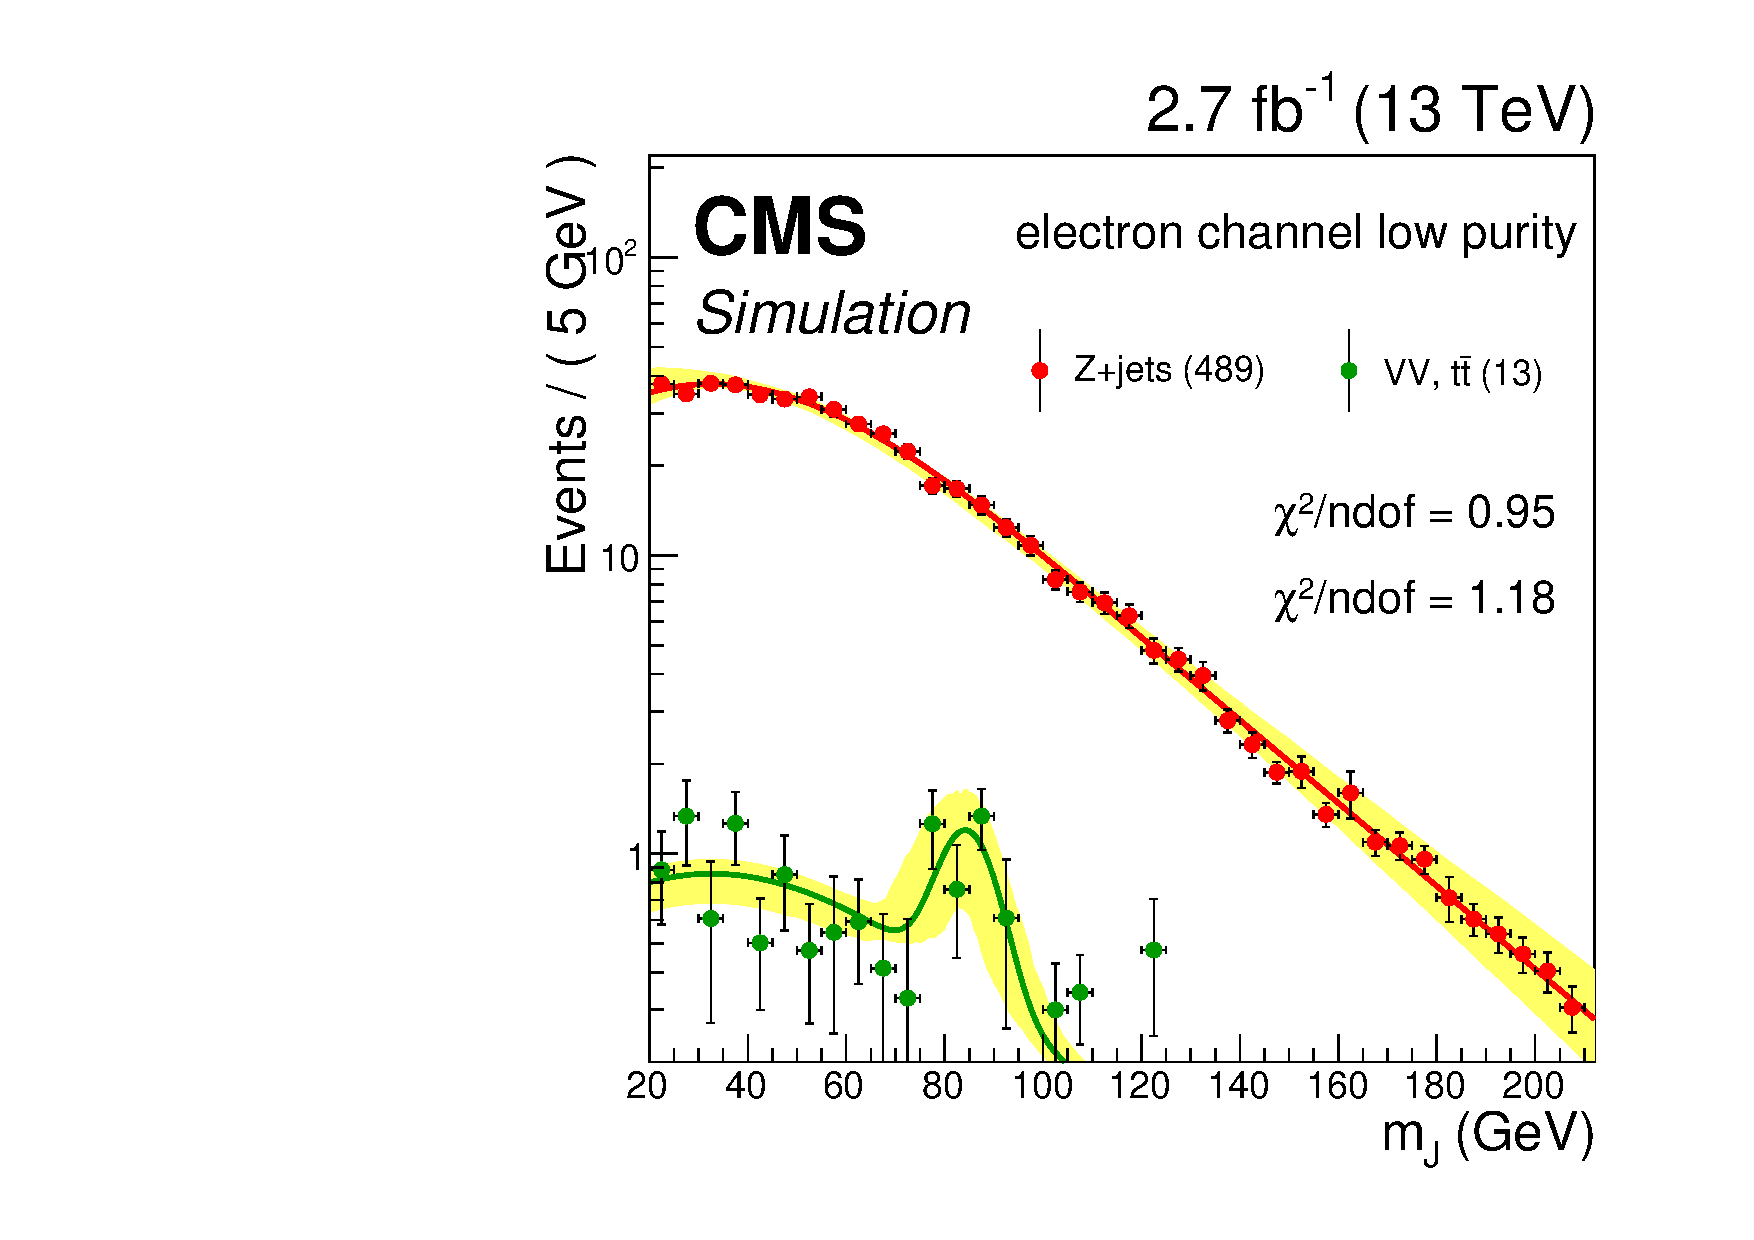
\includegraphics[width=0.47\textwidth]{figures/fits/bkgMjELP.pdf}\newline
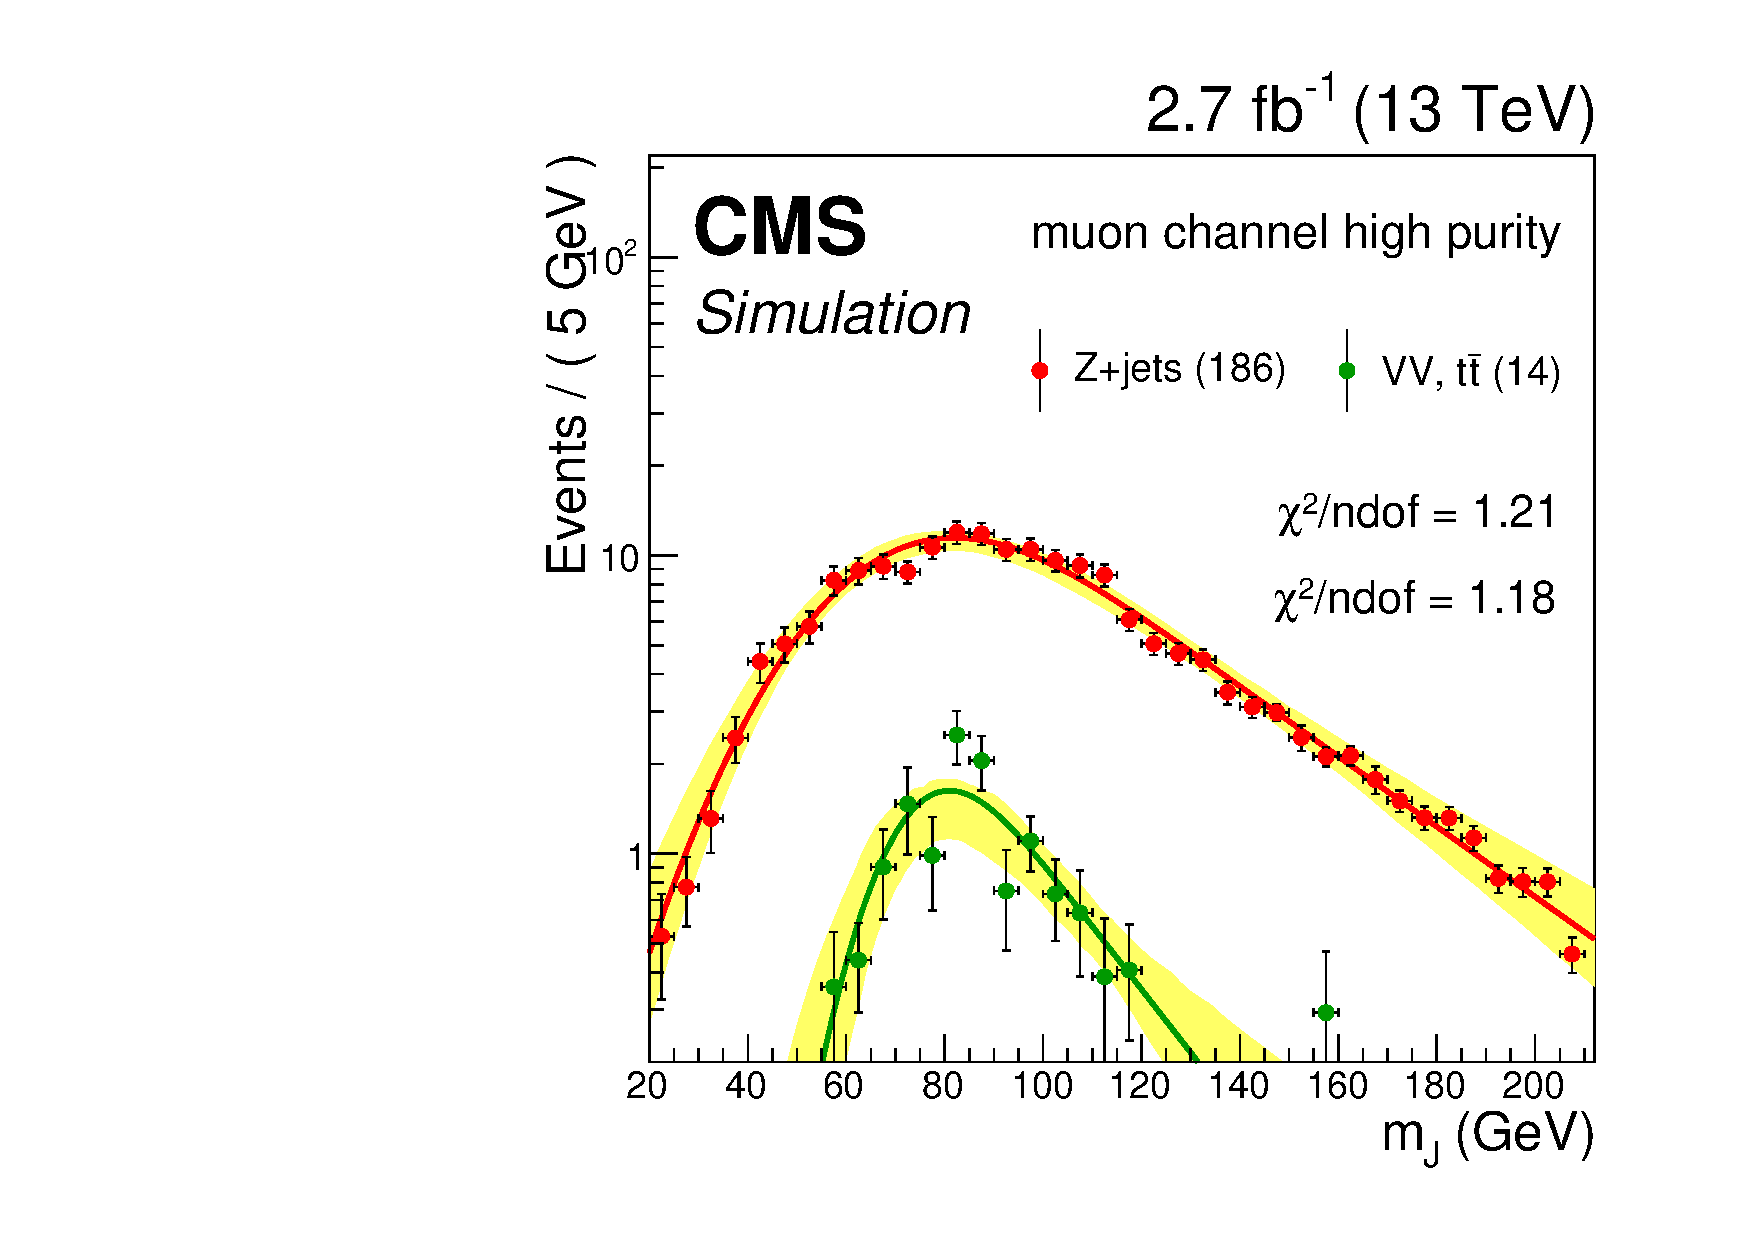
\includegraphics[width=0.47\textwidth]{figures/fits/bkgMjMHP.pdf}
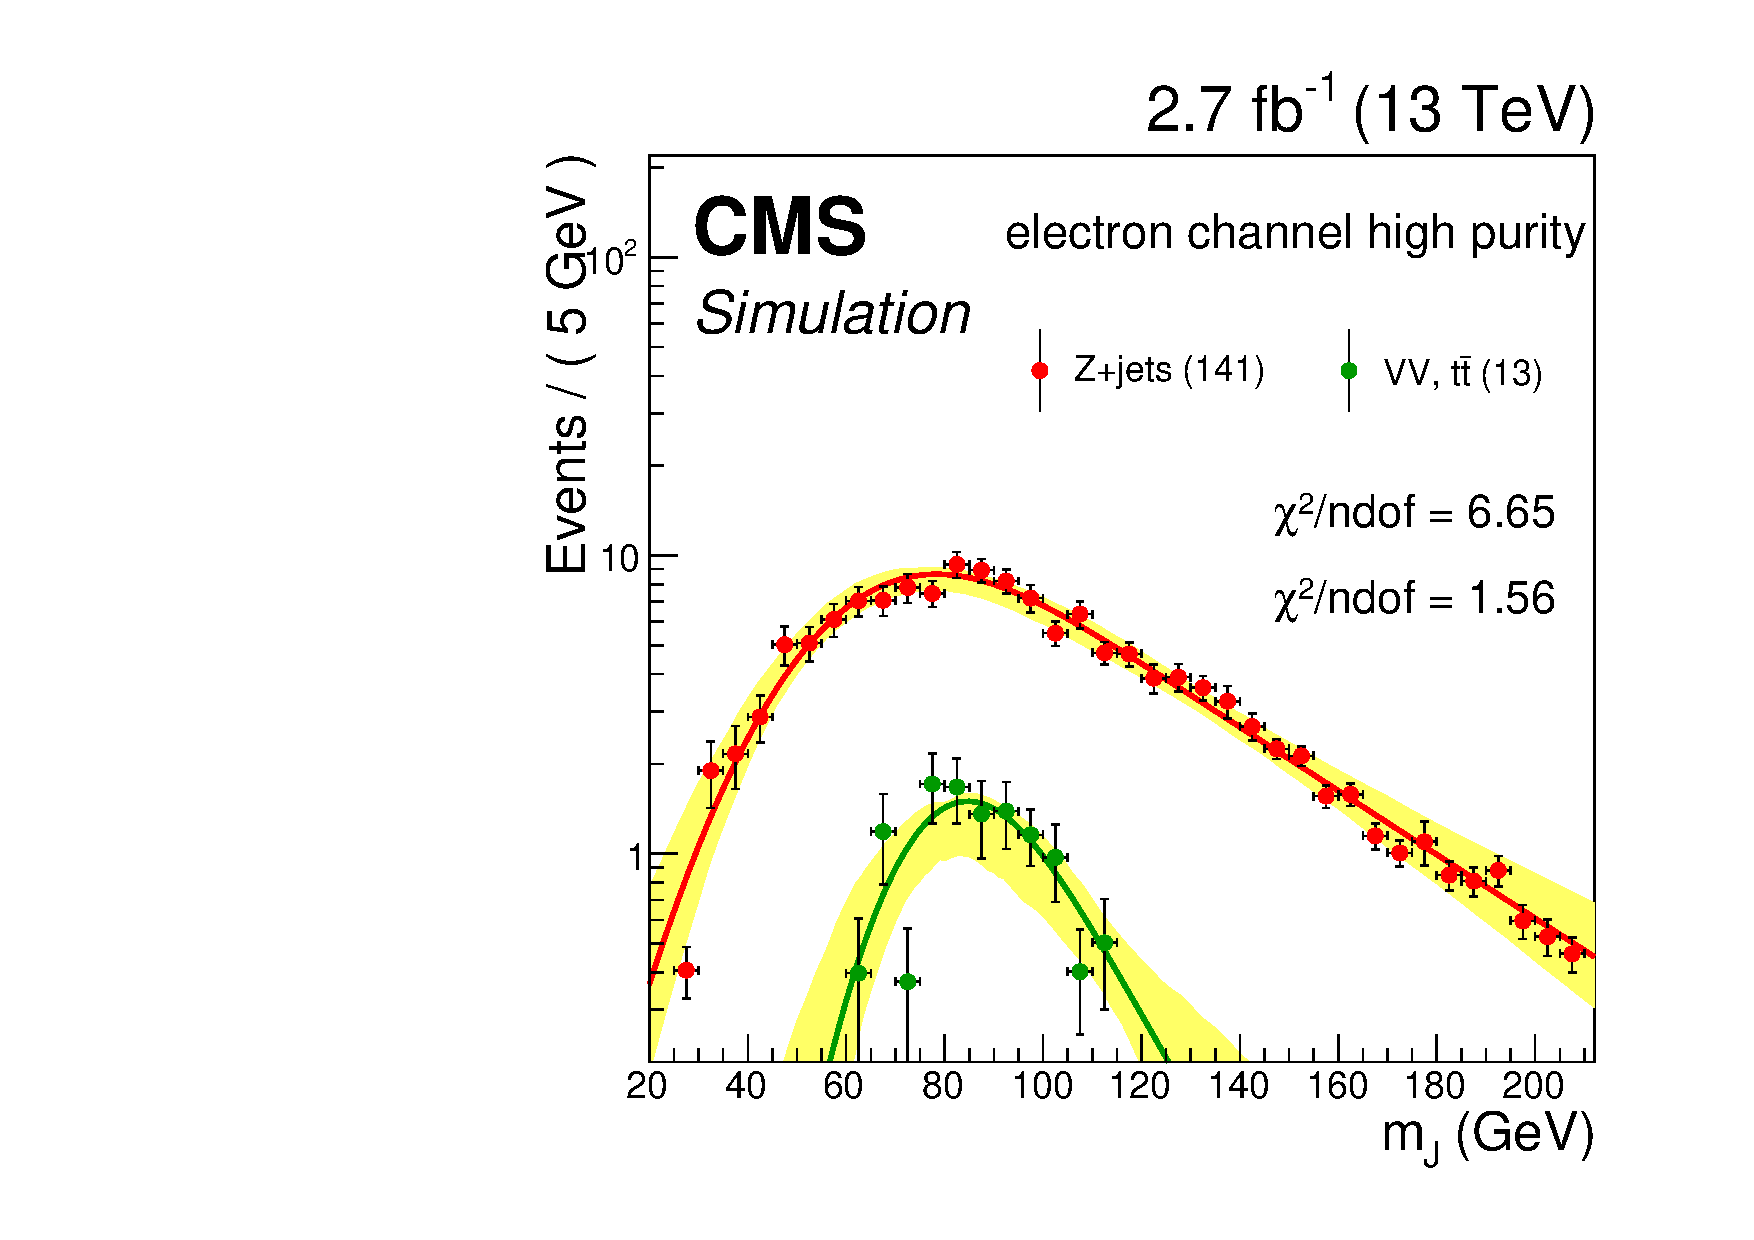
\includegraphics[width=0.47\textwidth]{figures/fits/bkgMjEHP.pdf}\newline
\caption[Jet mass fits in MC]{Fits of the jet mass for the dominant and subdominant components of the background using MC simulation.}
\label{fig:fits_MJ}
\end{figure}

\begin{figure}[hb!]
\begin{center}
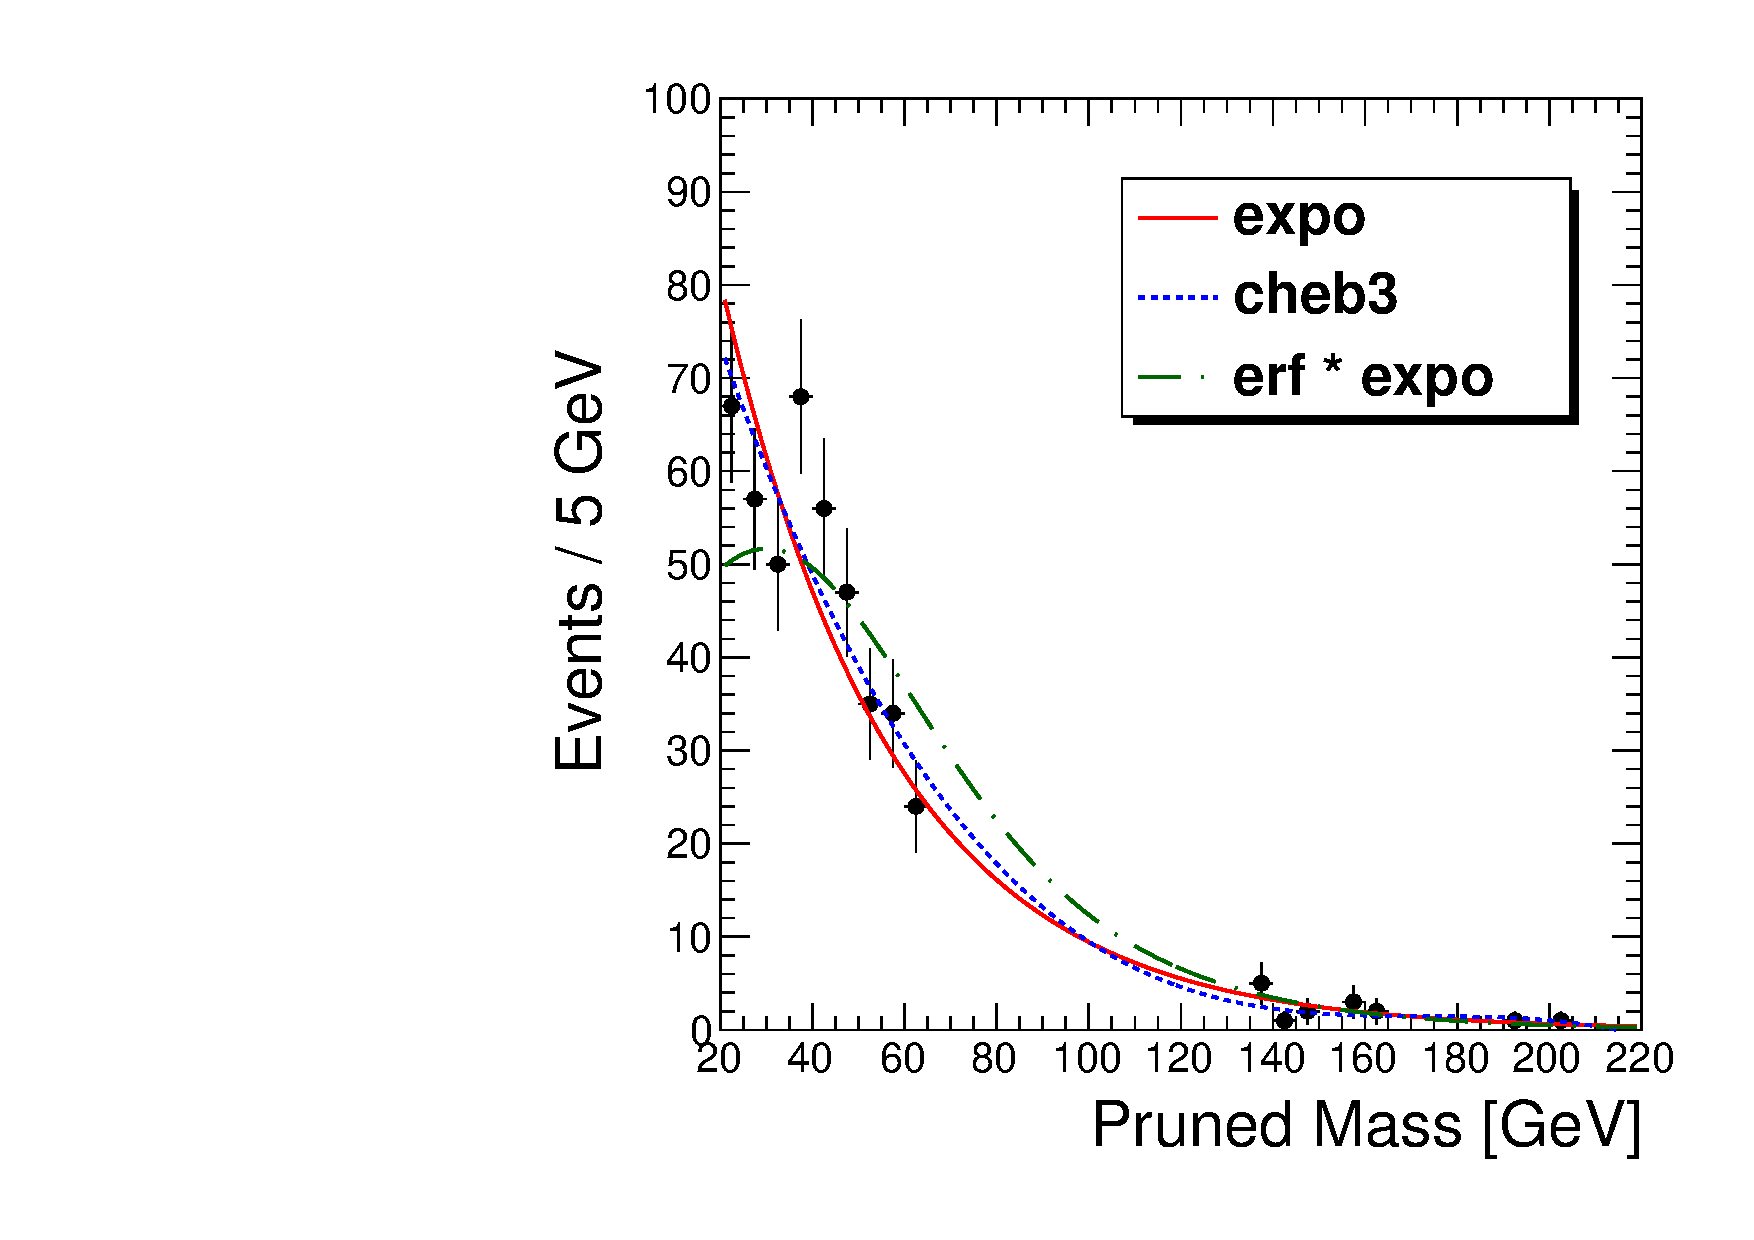
\includegraphics[width=0.47\textwidth]{figures/fits/thiagoFitMLP.pdf}
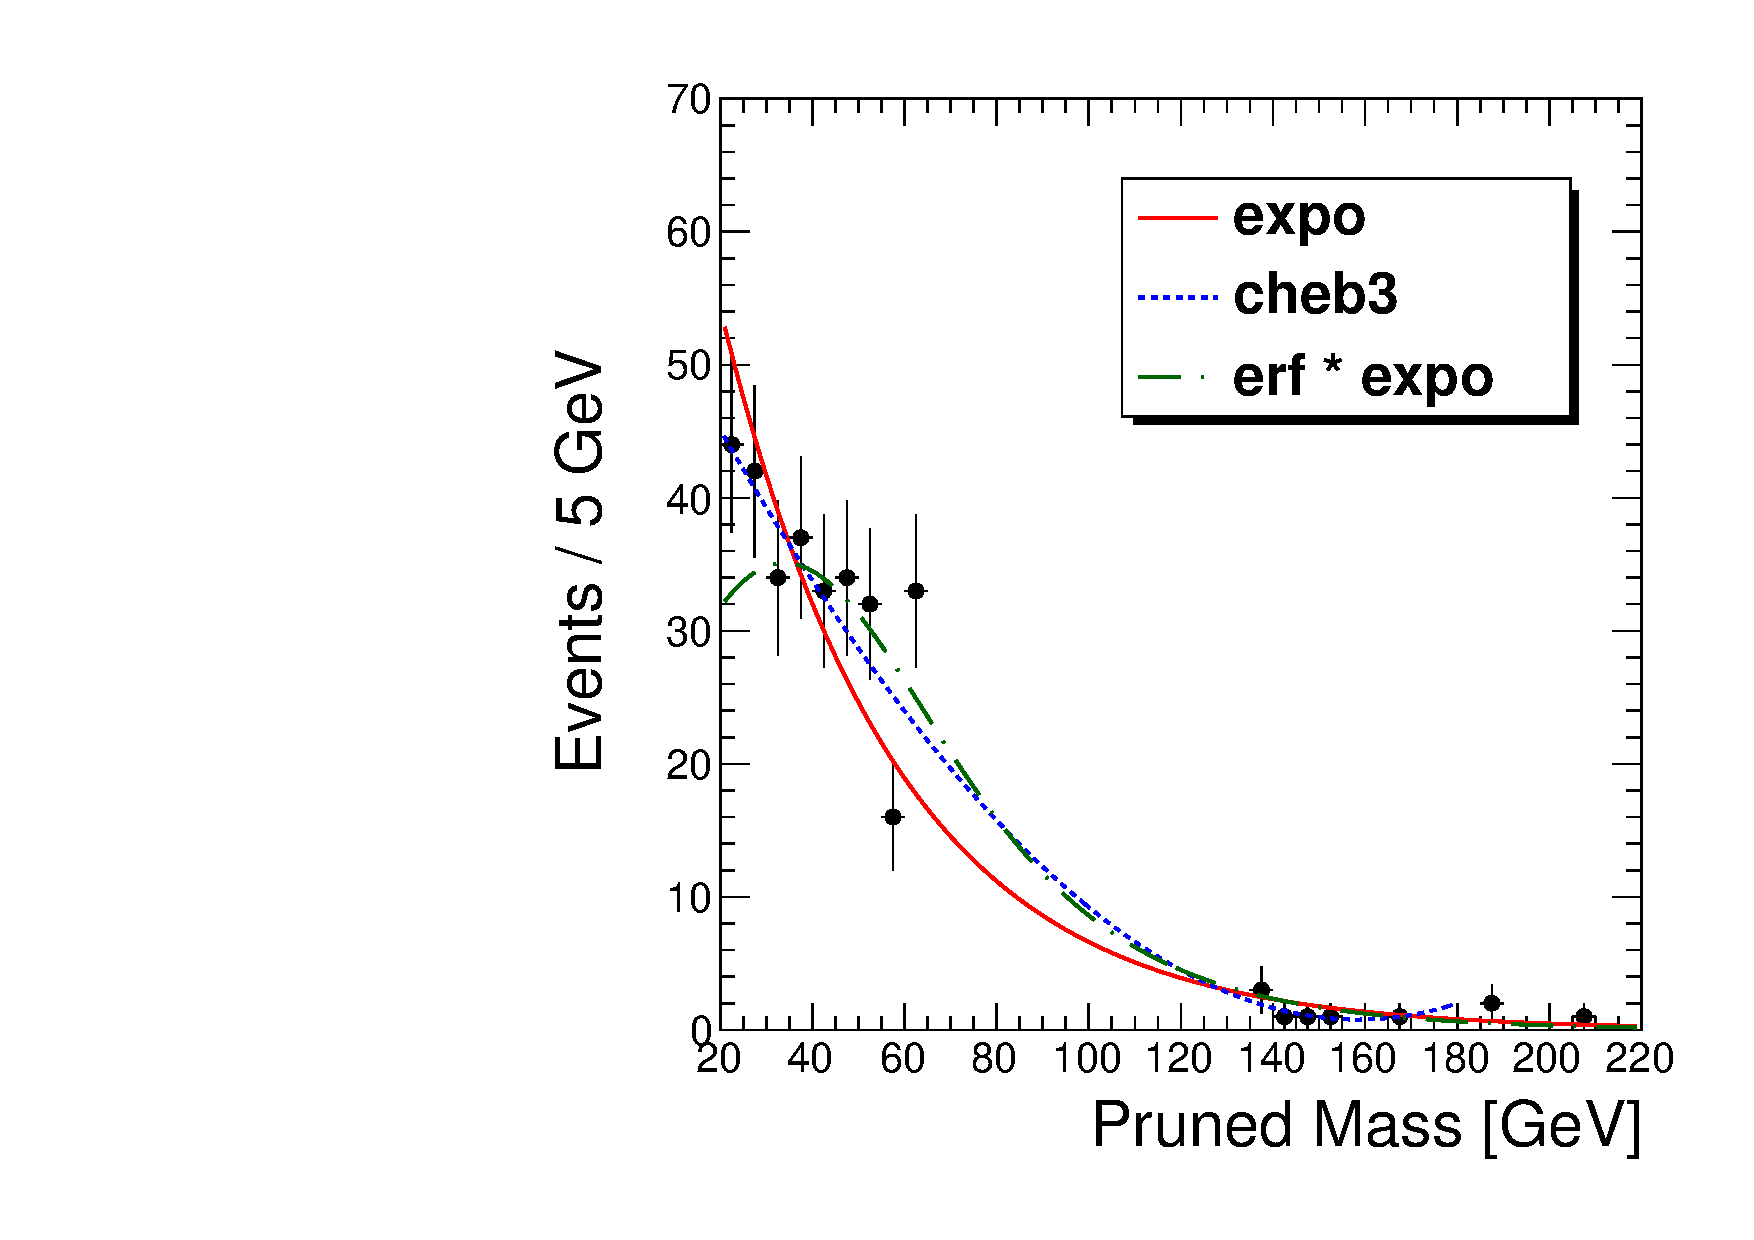
\includegraphics[width=0.47\textwidth]{figures/fits/thiagoFitELP.pdf}\\
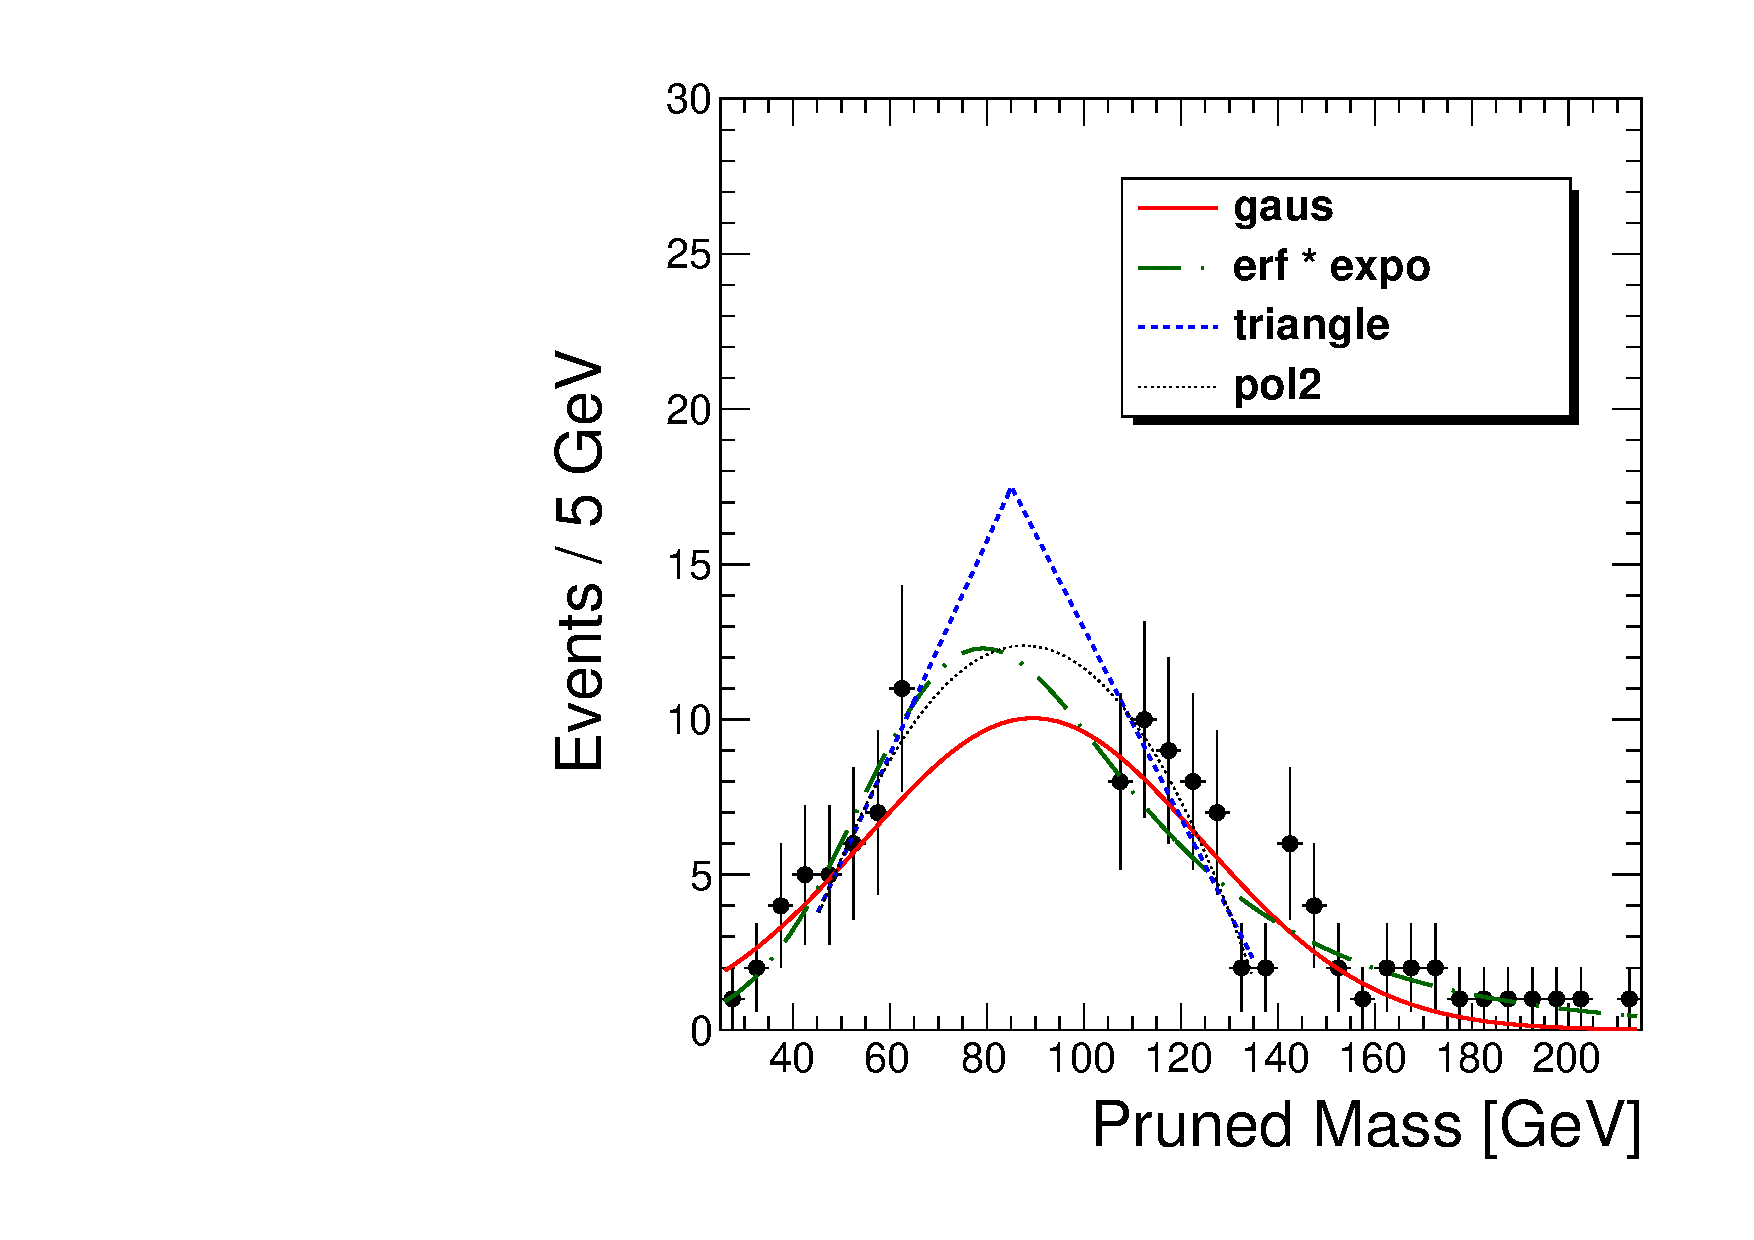
\includegraphics[width=0.47\textwidth]{figures/fits/thiagoFitMHP.pdf}
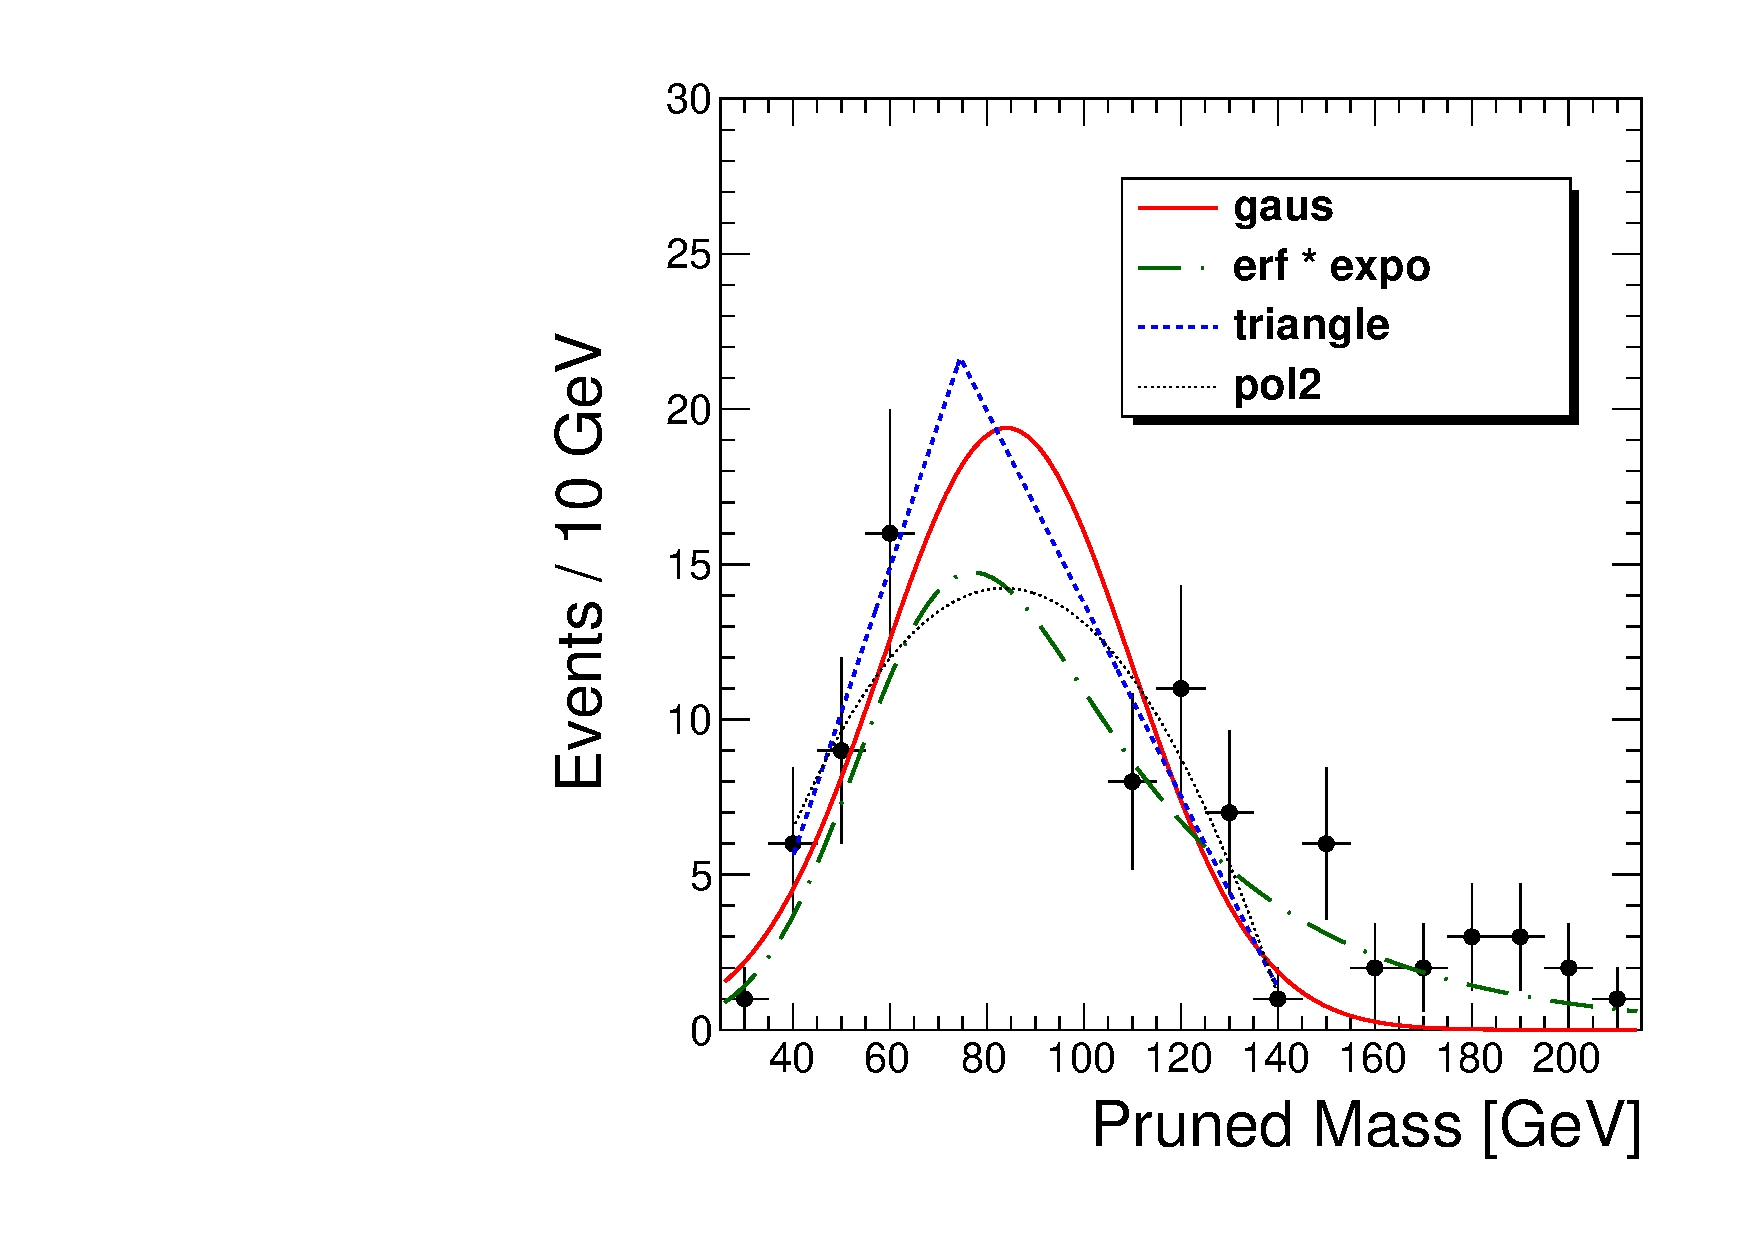
\includegraphics[width=0.47\textwidth]{figures/fits/thiagoFitEHP.pdf}
\caption[Jet mass fits in data]{Fit of the jet mass using different models to estimate the systematic uncertainty in the background normalization. The categories are: muon low purity (top-left), electron low purity (top-right), muon high purity (bottom-left), and electron high purity (bottom-right).}
\label{thiagoFits}
\end{center}
\end{figure}

\clearpage
\section{Unblind of the Signal Region}
Fig.~\ref{mjFit_VZ} shows the jet mass distribution in data and the parametric model made out of two components. The dominant component accounts for the Z+jets background, and the subdominant component corresponds to diboson VV and $t\bar{t}\,$ background. The parametric model consists of an error function multiplied by an exponential (ErfExp); in the low-purity categories a gaussian on top of the ErfExp is used for modeling the subdominant backgrounds. The goodness of this choice was evaluated first in simulation as demonstrated in Fig. \ref{fig:fits_MJ}. The small panel below every plot contains a pull histogram between the data and the adjusted model. Additionally, Table \ref{dataMCunblind} contains the event yields and Data/MC ratios including the signal region.

The description of the jet mass with the parametric model was tested in simulation and compared against alternative functions. To account for the mismodeling of the jet mass, an uncertainty was added as a systematic error that ranges between 28-42\%. The expected number of events in the signal region is given in Table~\ref{tab:bkgnormal} for the categories muon low purity (MLP), electron low purity (ELP), muon high purity (MHP), and electron high purity (EHP). The estimated background is reported in the format A $\oplus$ B, where A  and B represent the dominant and subdominant components, respectively.

\begin{table}[h!]
\begin{center}
\caption[Data/MC ratios after unblind]{Events yields and Data/MC ratios including the signal region.}
\label{dataMCunblind}
\begin{tabular}{lccc}
\hline\\[-0.2cm]
\textbf{Category}    & \textbf{Data} & \textbf{MC}   &\textbf{Data/MC} \\[0.2cm]
\hline\hline\\[-0.2cm]
Muon Low Purity      & 592           & 596           & 0.993 \\[0.2cm]
Muon High Purity     & 222           & 208           & 1.067 \\[0.2cm]
Electron Low Purity  & 412           & 412           & 0.999 \\[0.2cm]
Electron High Purity & 155           & 130           & 1.192 \\[0.2cm]
\hline
\end{tabular}
\end{center}
\end{table}

\begin{figure}[p]
\begin{center}
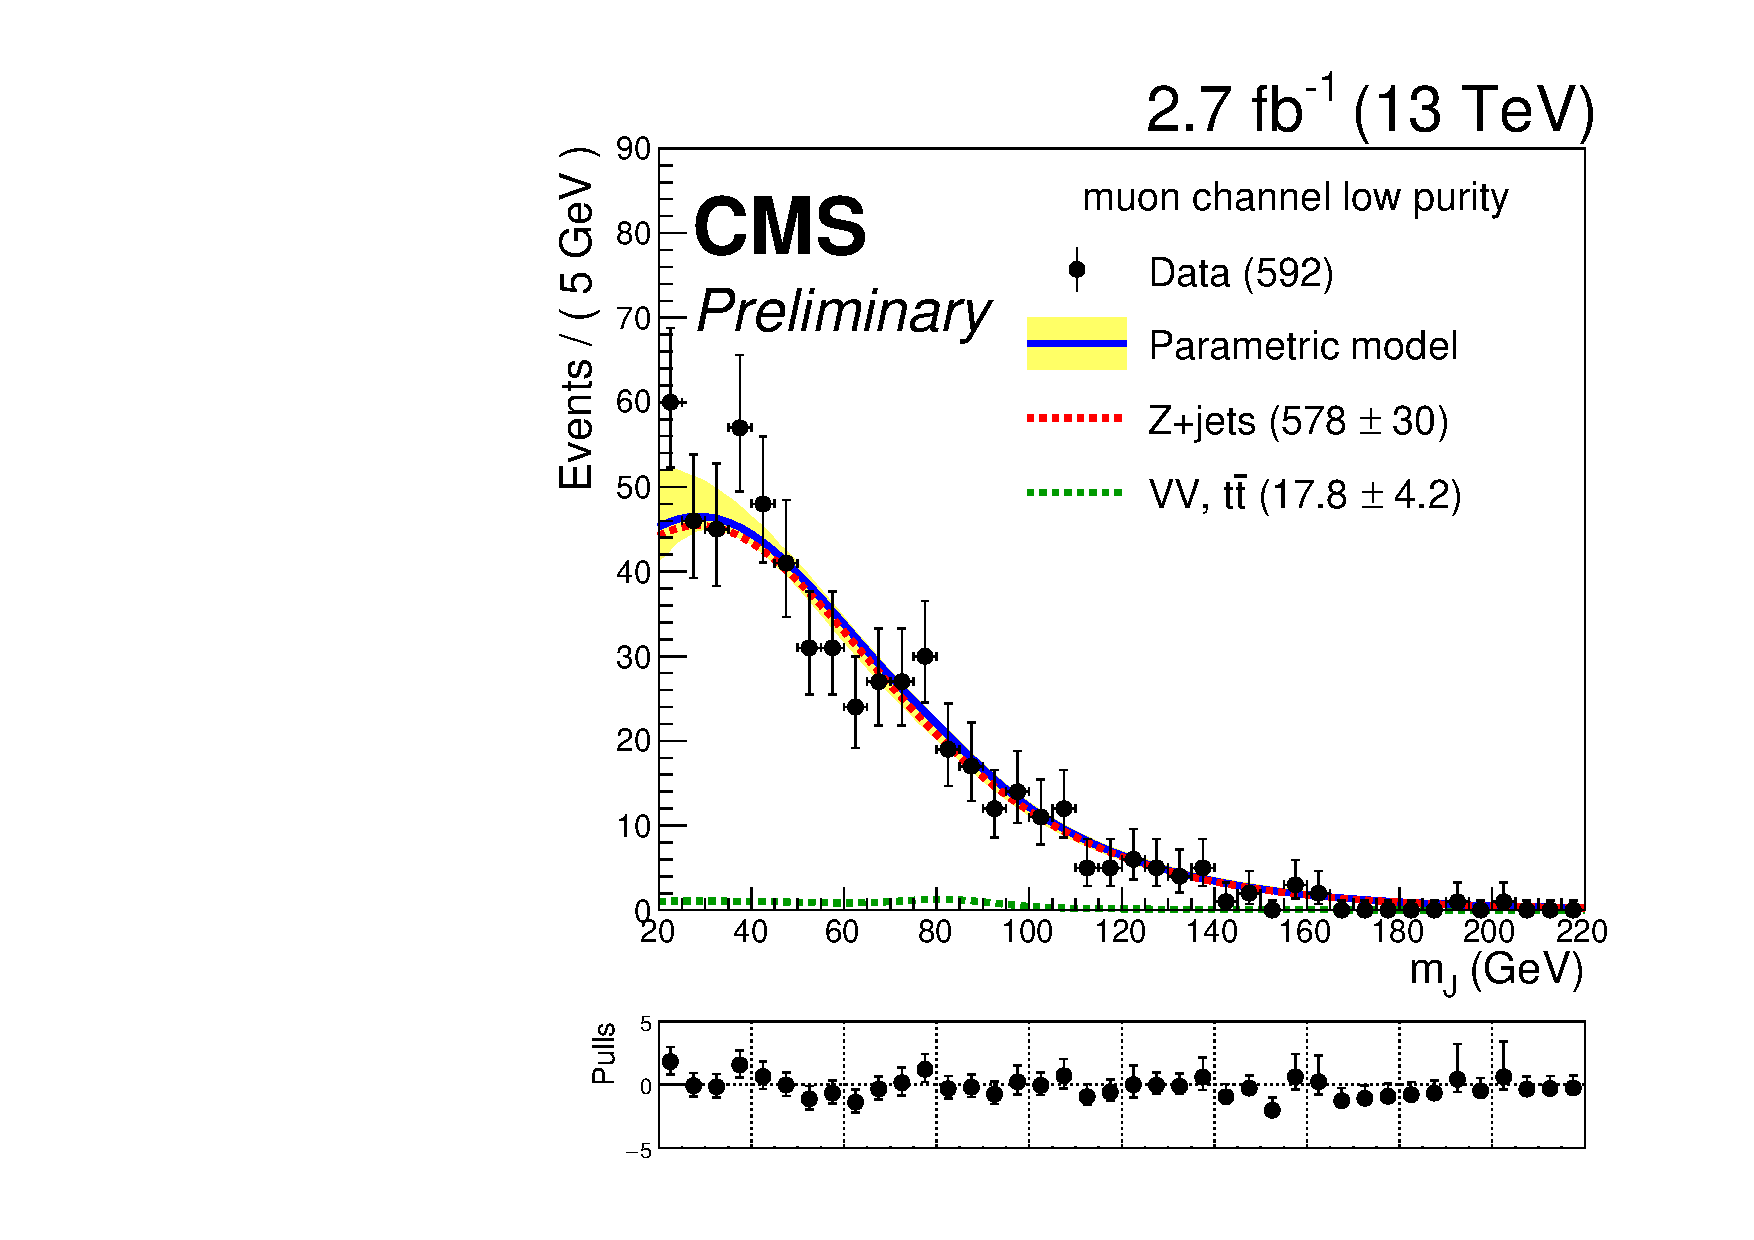
\includegraphics[width=0.47\textwidth]{figures/fits/mjFitMLP.pdf}
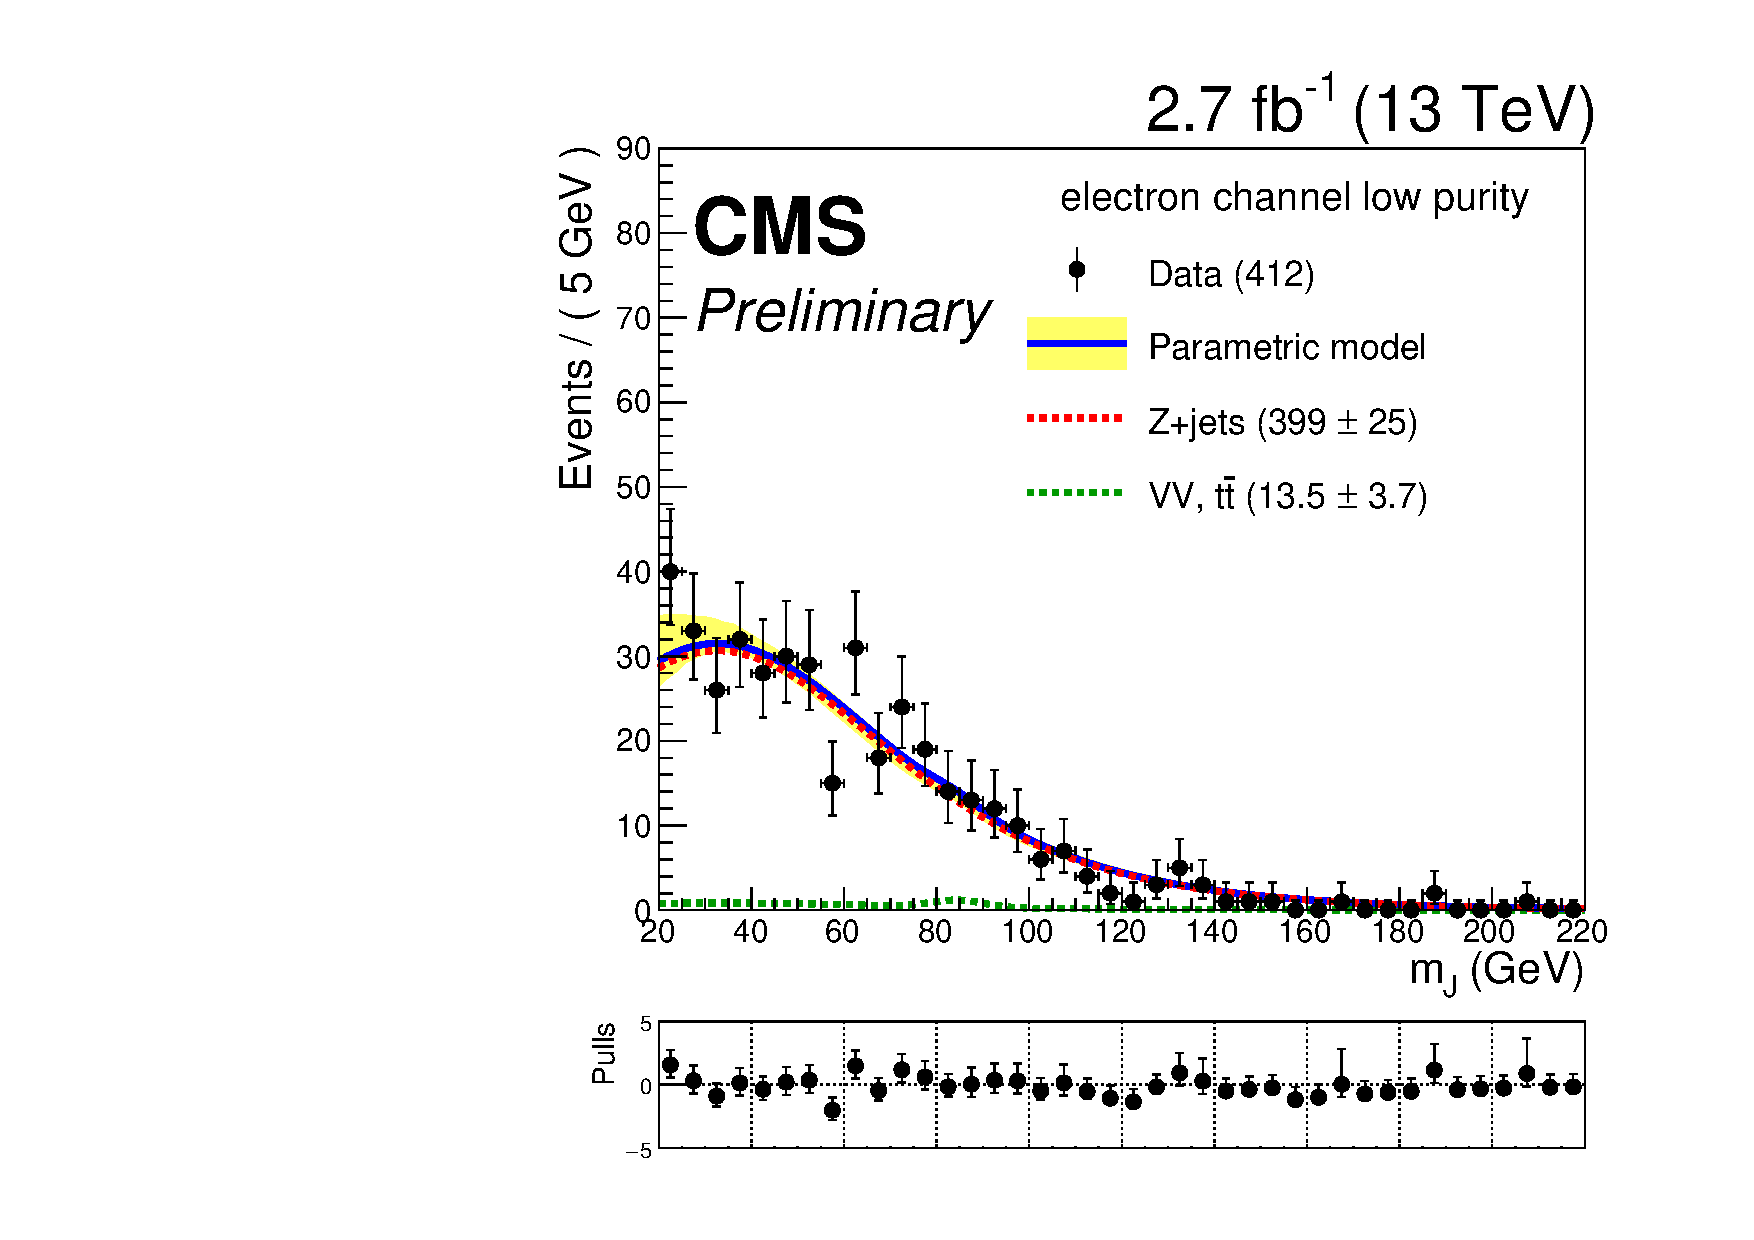
\includegraphics[width=0.47\textwidth]{figures/fits/mjFitELP.pdf}\\
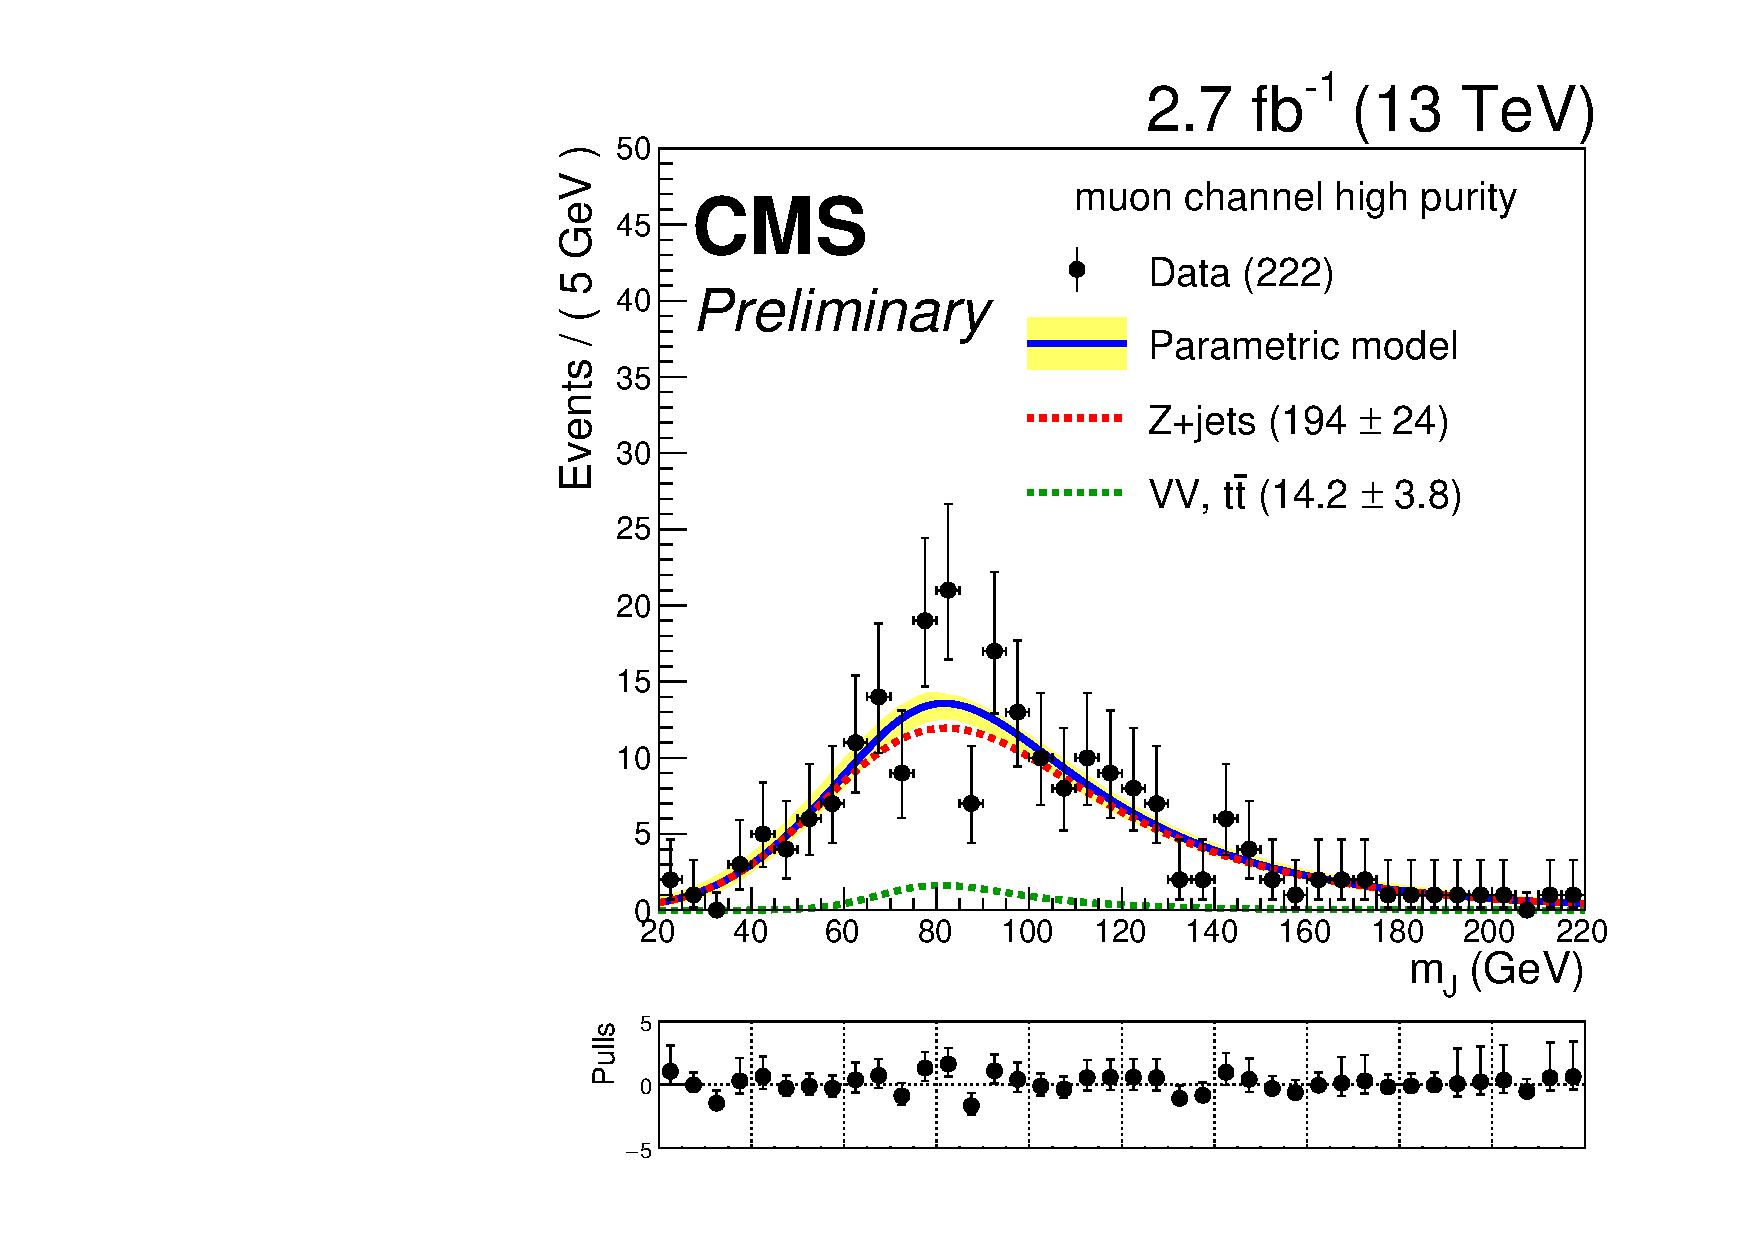
\includegraphics[width=0.47\textwidth]{figures/fits/mjFitMHP.pdf}
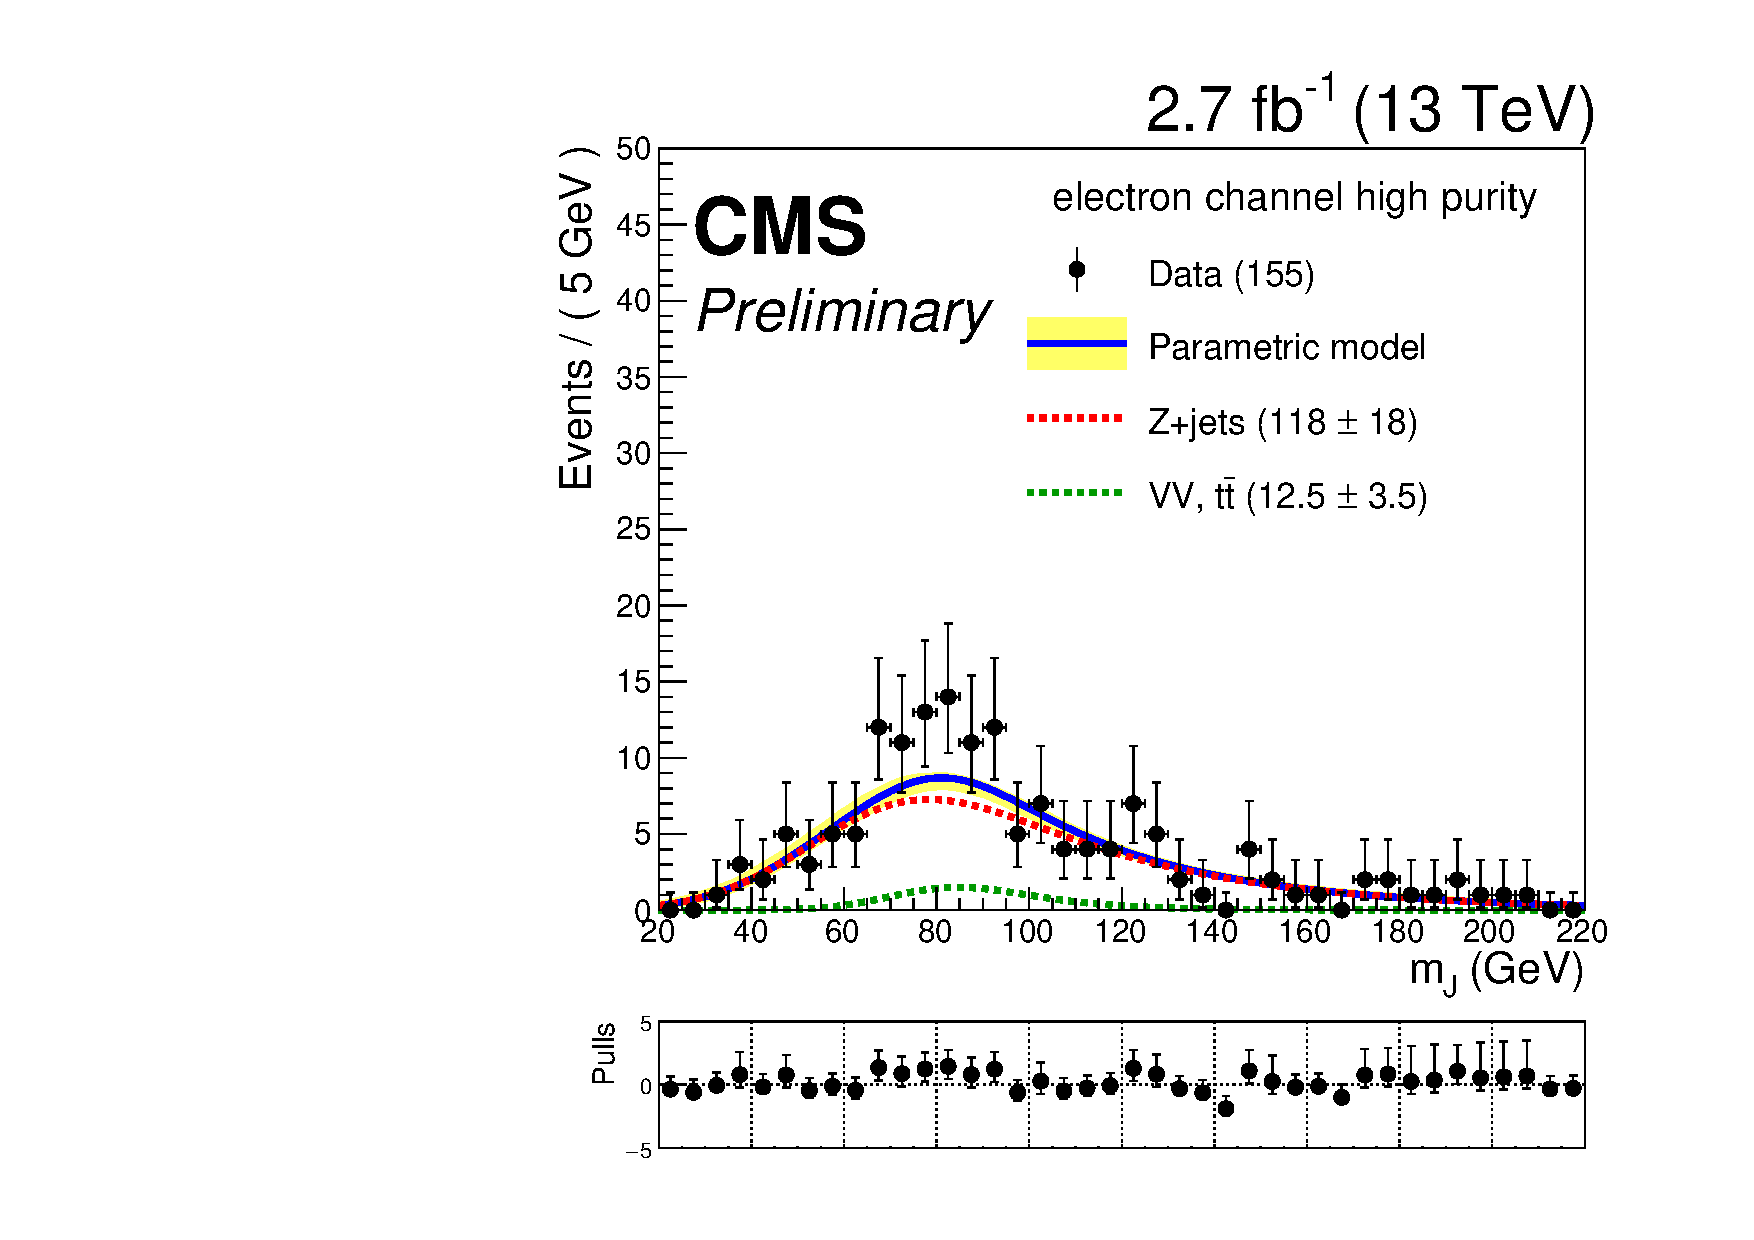
\includegraphics[width=0.47\textwidth]{figures/fits/mjFitEHP.pdf}
\caption[Jet mass distribution]{Jet mass distribution in data and parametric model (blue line). The dominant (red) and subdominant (green) components are also shown. The yield for each component in the full region ($20 < \mj < 220$ GeV) is written in the legend.}
\label{mjFit_VZ}
\end{center}
\end{figure}

\begin{landscape}
\begin{table}[p]
%\footnotesize
\begin{center}
\caption[Estimated background in the signal region for different models.]{Estimated background in the signal region for different models and associated uncertainty.}
\label{tab:bkgtest}
\begin{tabular}{cccccccccc}
\hline\\[-0.3cm]
	       &   Exp    & Chebychev 3  &    ErfExp   &   Gaus   & Polynomial 2 & Triangle & $\frac{\rm largest-smallest}{\rm smallest}$  & $\frac{\rm largest-smallest}{\rm largest}$  & $\Delta$     \\[0.2cm] \hline\hline 
   MLP     &   118    &      129            &    162        &      -       &         -            &       -       &            37\%        &        27\%          &       32\%   \\ 
   ELP     &   82      &       100           &    114        &      -       &         -            &       -       &            39\%         &        28\%          &        34\%    \\ 
   MHP    &   -         &         -             &      89         &    76      &       94           &  114       &            50\%         &        33\%         &        42\%     \\ 
   EHP     &  -          &        -              &      53         &    70     &        55           &    70        &            32\%        &        24\%         &         28\%    \\ \hline
\end{tabular}
\end{center}
\end{table}

\begin{table}[p]
%\scriptsize
%\footnotesize
\begin{center}
\caption[Background estimation]{Background estimation obtained by the integral of the parametric model in the signal region ($65 < \mj < 105$ GeV). The estimated background is reported in the format A $\oplus$ B, where A  and B represent the dominant and subdominant components, respectively. The systematic uncertainty due to mismodeling of the jet mass ranges between 28-42\%.}
\label{tab:bkgnormal}
\begin{tabular}{ c  ccl  ccc  c  c }
\hline\\[-0.3cm]
Category & \multicolumn{3}{c}{Parametric model}      &\multicolumn{3}{c}{Estimated background} & Syst. unc.      & Data in SR \\[0.1cm] \hline\hline 
   MLP     &   (ErfExp)  & $\oplus$ & (ErfExp + Gaussian)     &(150 $\pm$ 11) & $\oplus$ & (7.4 $\pm$ 3)            &          32 \%                &  157                \\ 
   ELP     &    (ErfExp)  & $\oplus$ & (ErfExp + Gaussian)    &(105 $\pm$ 10) & $\oplus$ & (5   $\pm$ 2)              &          34 \%                & 116                \\ 
   MHP     &   (ErfExp)  & $\oplus$ & (ErfExp)                       &(88 $\pm$ 8)     &$\oplus$  & (10 $\pm$ 3)               &          42 \%                & 110                \\ 
   EHP     &    (ErfExp)  & $\oplus$ & (ErfExp)                       &(53 $\pm$ 7)    & $\oplus$  & (9 $\pm$ 3)                 &          28 \%                & 85                  \\ \hline
\end{tabular}
\end{center}
\end{table}
\end{landscape}

\clearpage

The $\mZV$ distribution of data in the signal region and the final background estimation is shown in Fig.~\ref{fig:highmass_MVZ}. The decomposition of the parametric model into dominant and subdominant components is also shown. The error band in the parametric model accounts for the shape uncertainties due to the transfer factor and the uncertainties in the fit of the $\mZV$ distribution in data in the sideband region. The normalization uncertainty (between 28-42 \%) due to mismodeling of the jet mass is considered as a nuisance parameter in the statistical framework that calculates the expected limits. An expanded discussion of systematic uncertainties and the statistical treatment is giving in the following sections.

\begin{figure}[htbp]
\centering
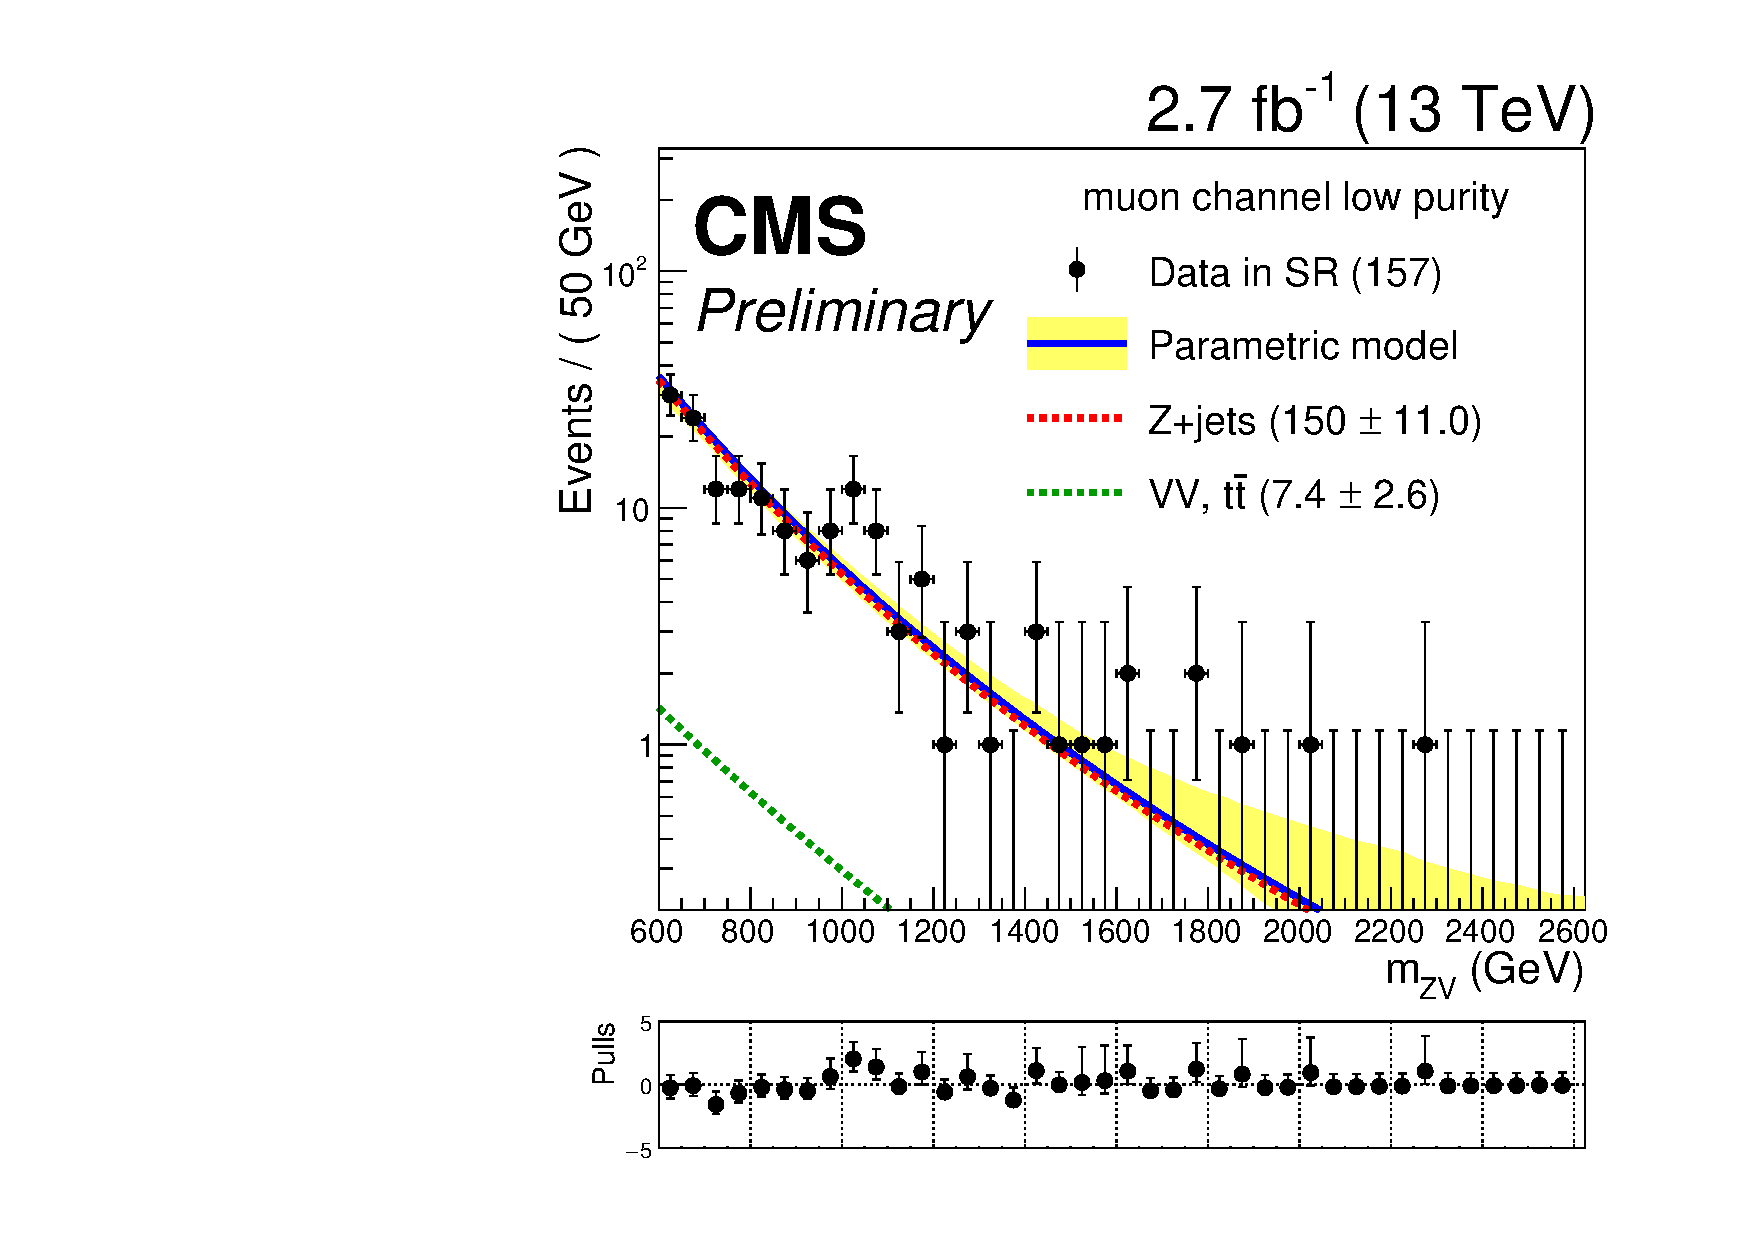
\includegraphics[width=0.47\textwidth]{figures/fits/mVZsigMLP.pdf}
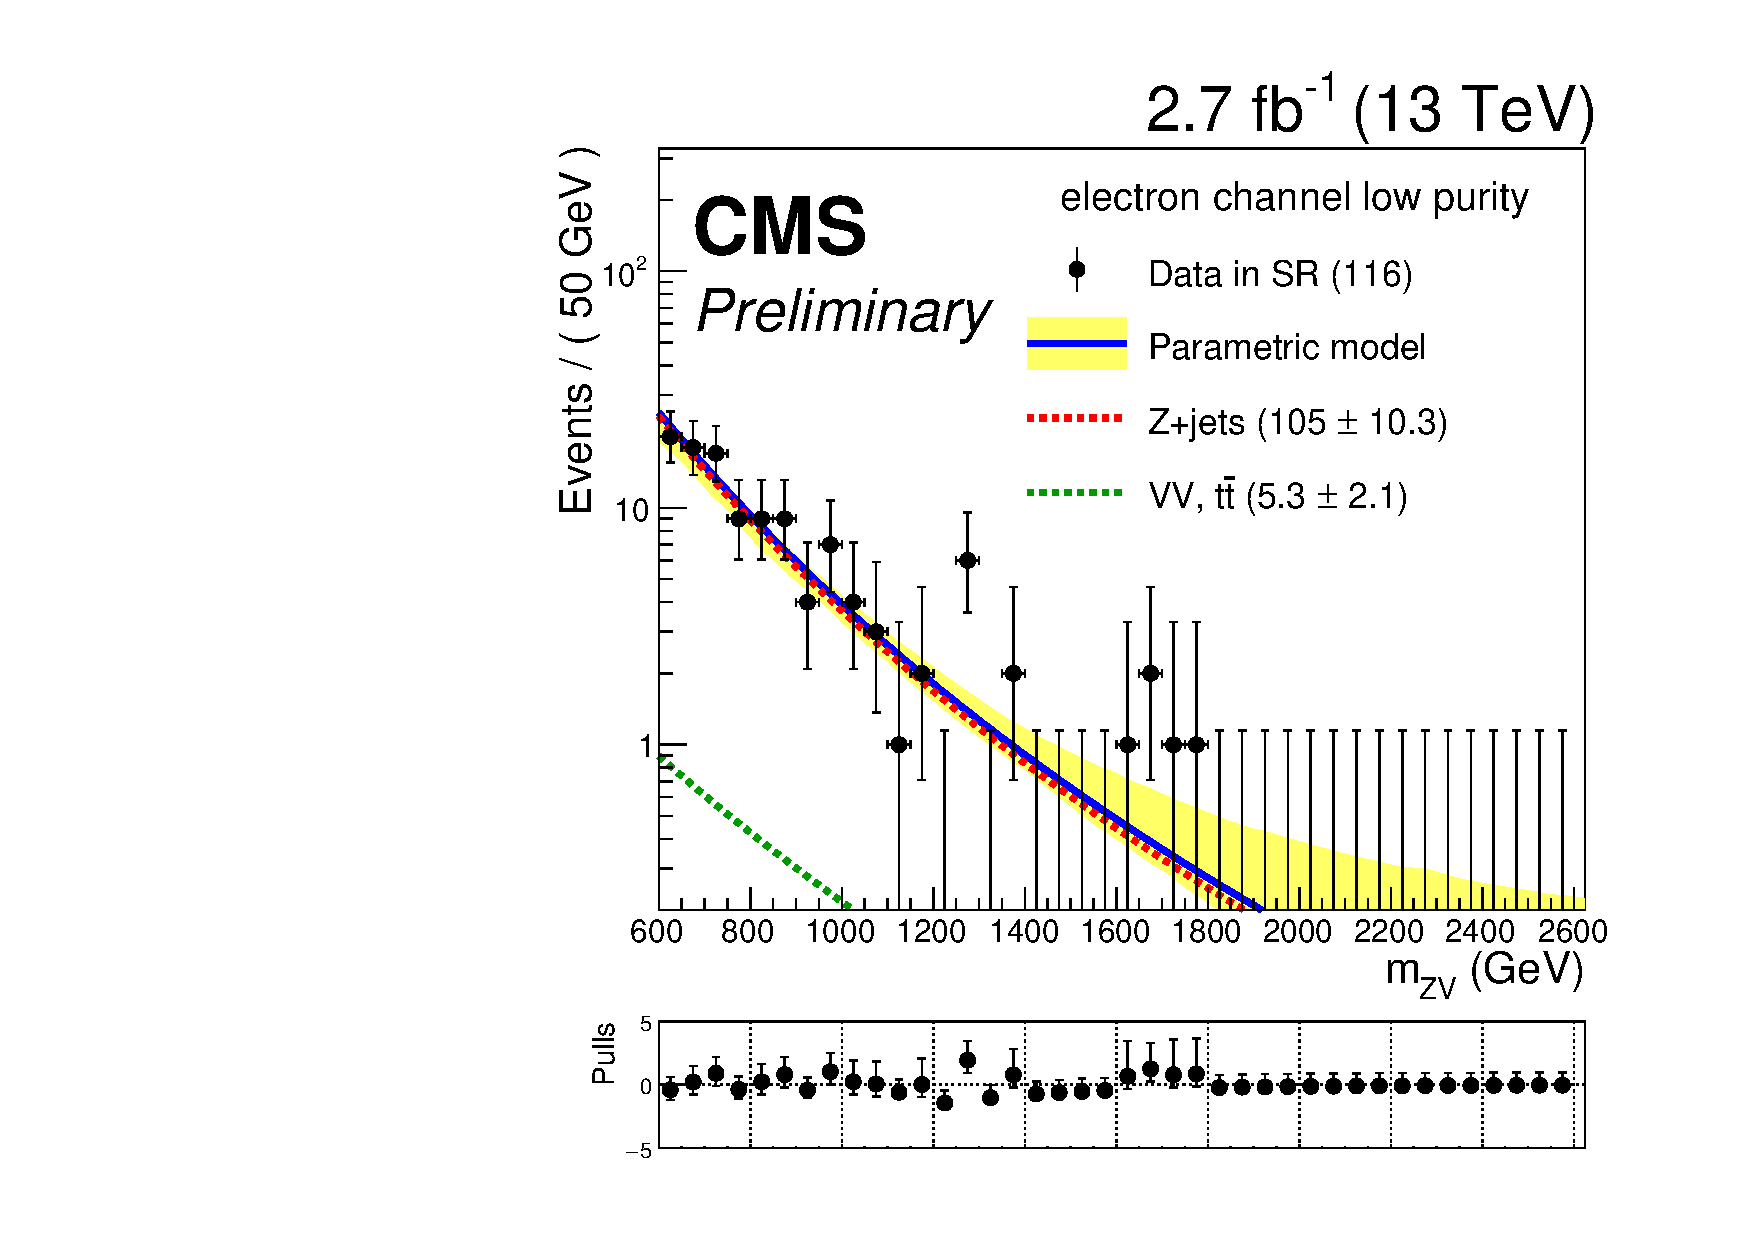
\includegraphics[width=0.47\textwidth]{figures/fits/mVZsigELP.pdf}\newline
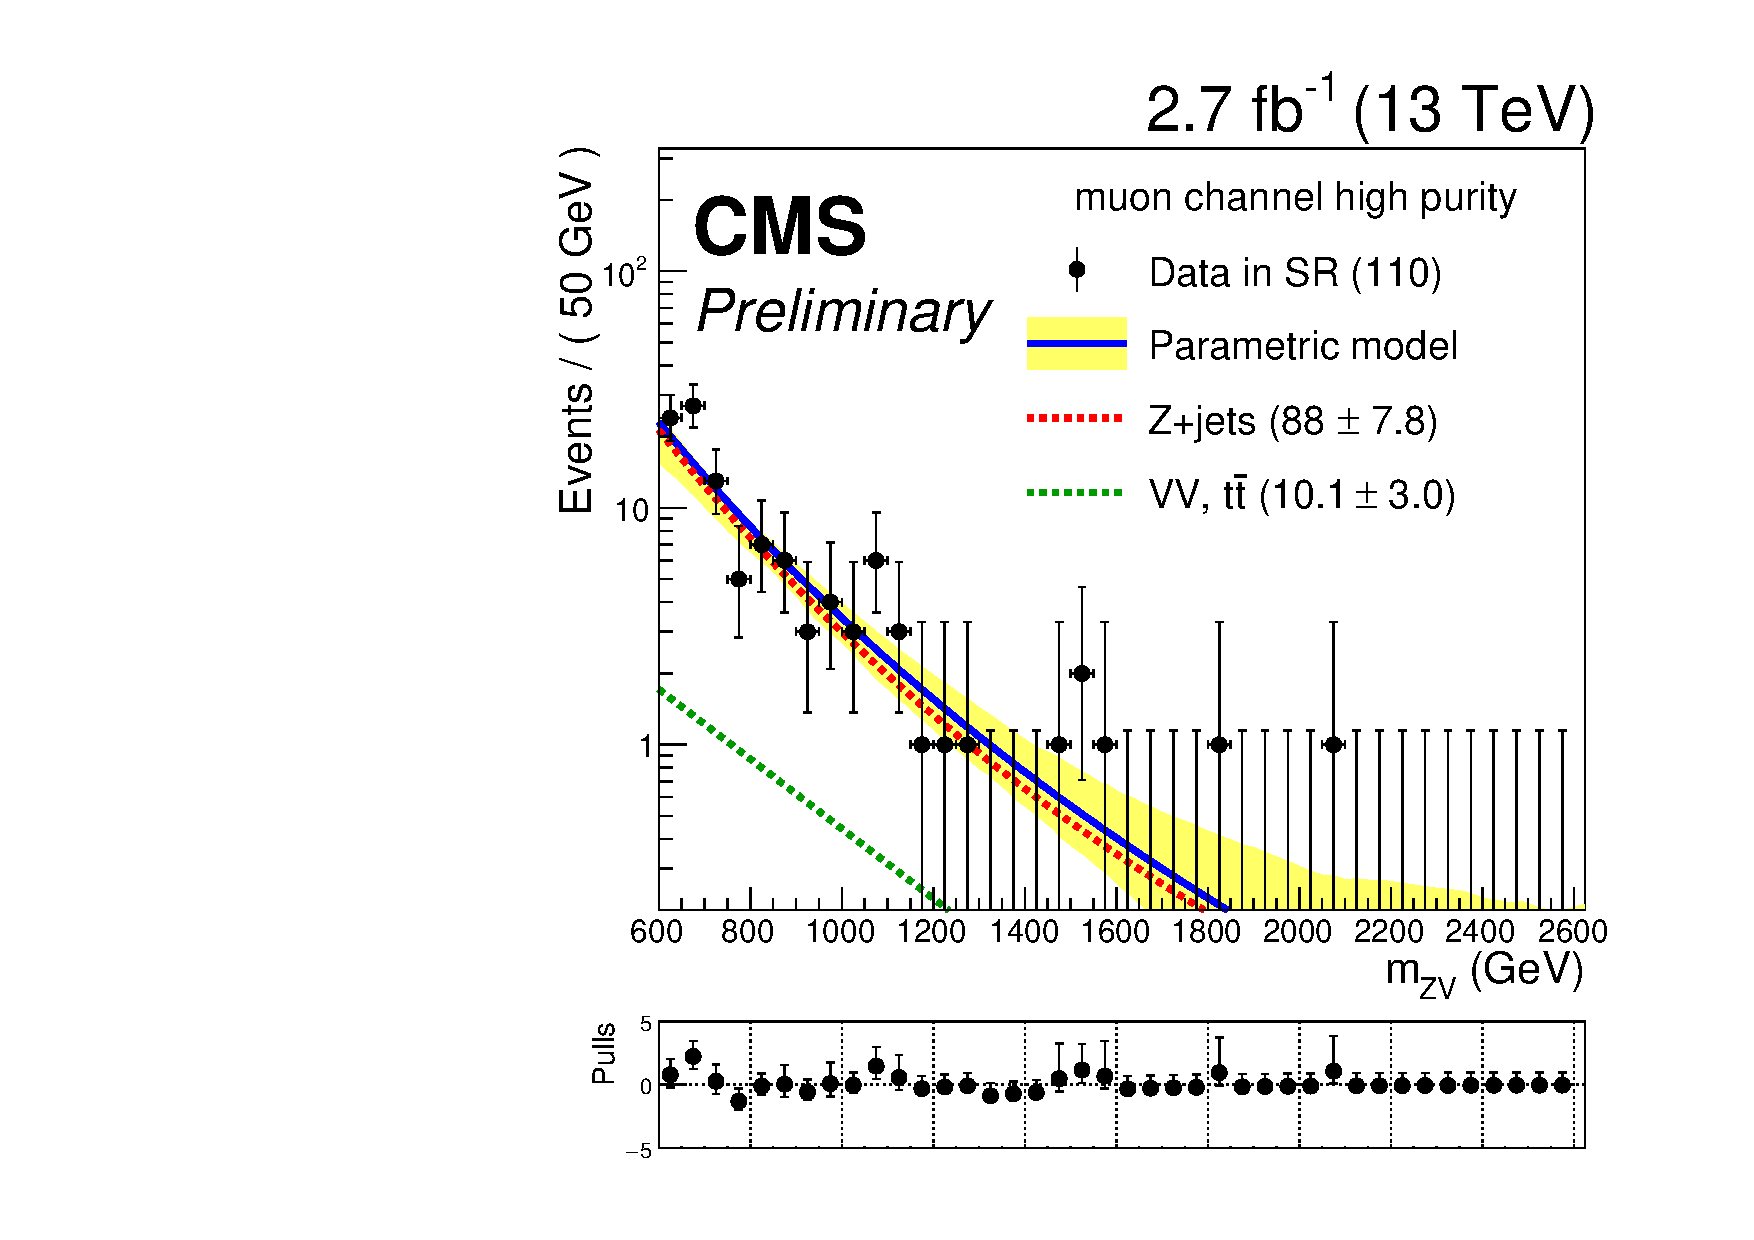
\includegraphics[width=0.47\textwidth]{figures/fits/mVZsigMHP.pdf}
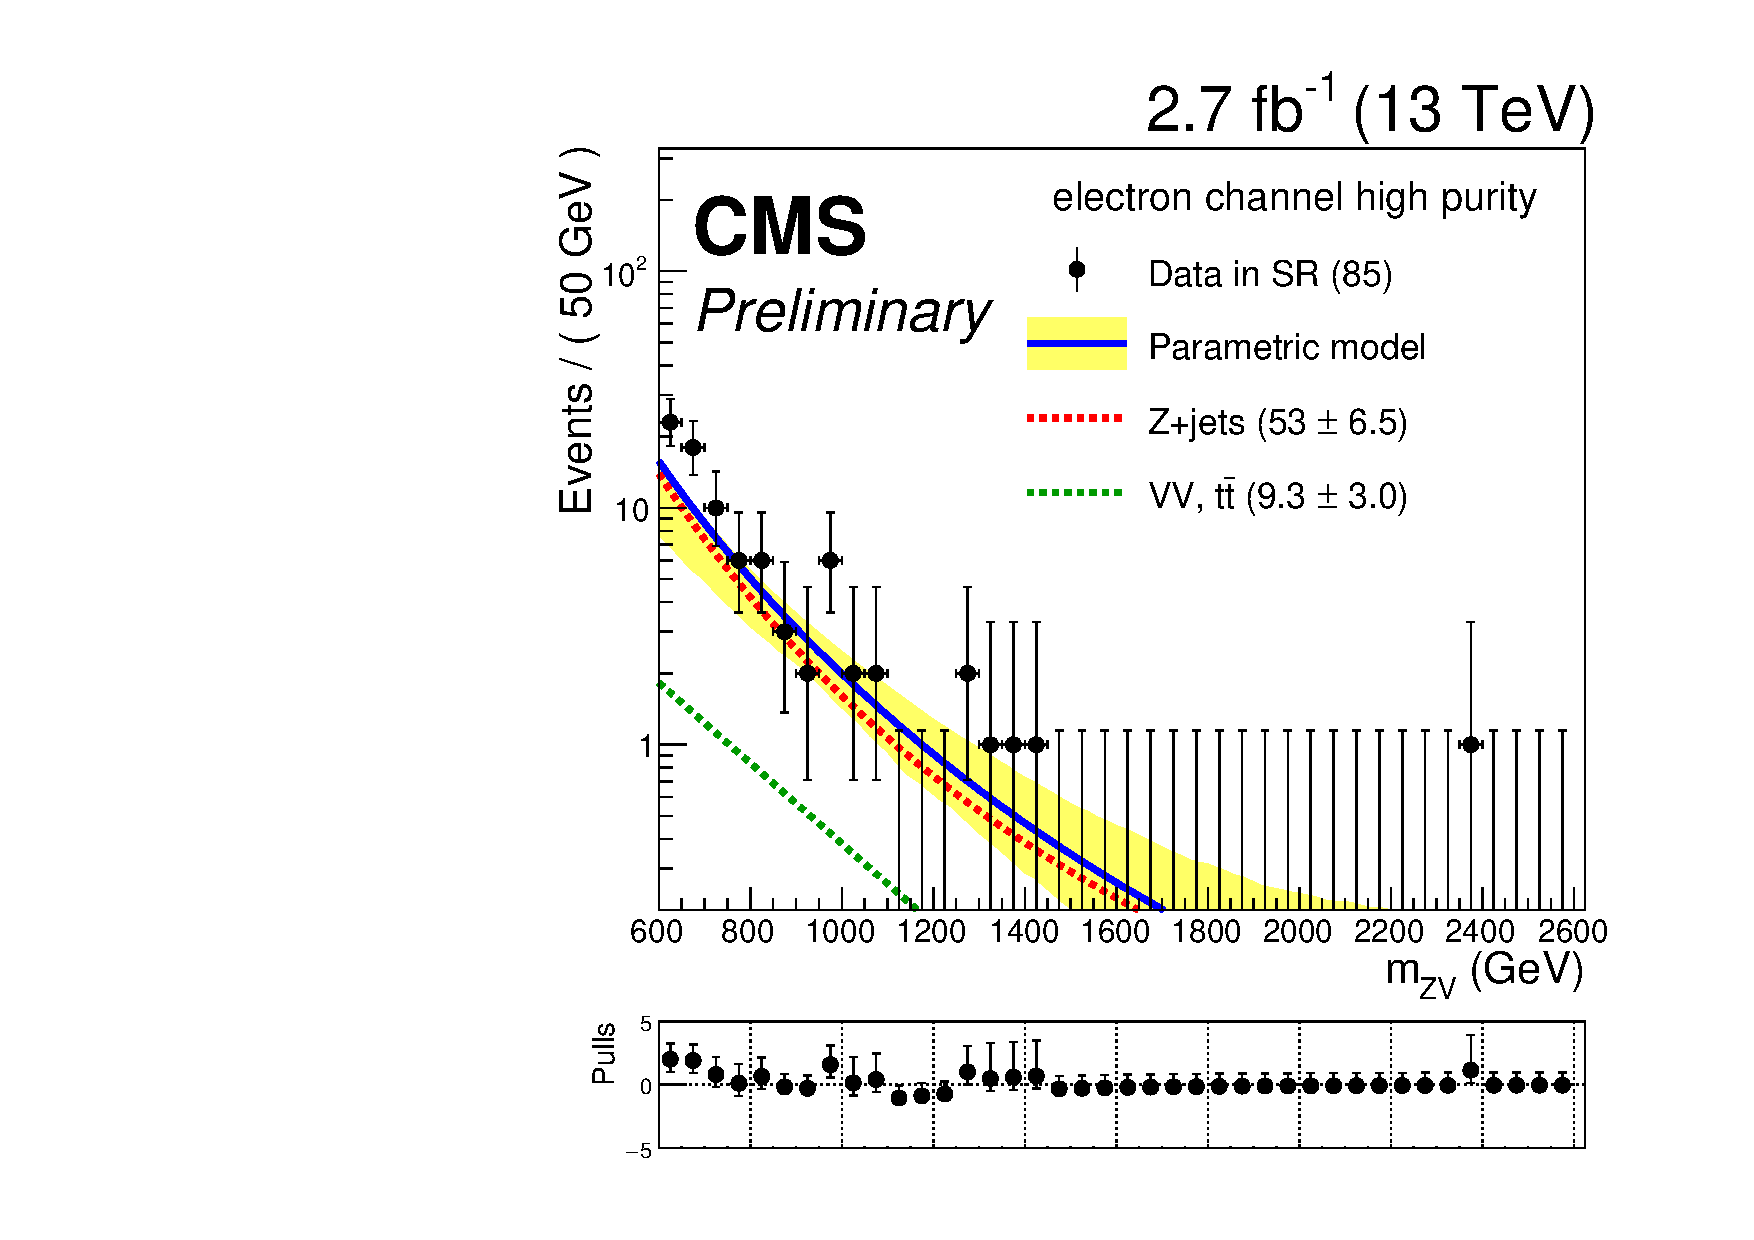
\includegraphics[width=0.47\textwidth]{figures/fits/mVZsigEHP.pdf}\newline
\caption[Invariant mass distributions]{
Top: $\mZV$ distributions in the signal region for the low purity category,
for muons (left) and electrons (right). 
Bottom: $\mZV$ distributions in the signal region for the high purity category,
for muons (left) and electrons (right). 
}
\label{fig:highmass_MVZ}
\end{figure}

\clearpage
\section{Systematic Uncertainties}
\label{sec:systematics}

A graviton with mass $M_G$ is expected to decay into a pair of Z bosons with $\ptrans\sim M_G/2$ each, as verified in the distribution of the Z boson $\ptrans$ at generator and reconstructed level shown in Fig. \ref{signal1TeV} . The mean value of the Z boson \ptrans in Fig. \ref{signal1TeV} is compared with the reconstructed jet \ptrans for two scenarios: with and without applying the jet energy corrections recommended by the JetMET physics object group \cite{jetmetPOG}. As expected, the jet energy corrections improve the agreement between reconstruction and generator level, both for the jet \ptrans and the jet mass distributions.  

\begin{figure}[htb]
\centering
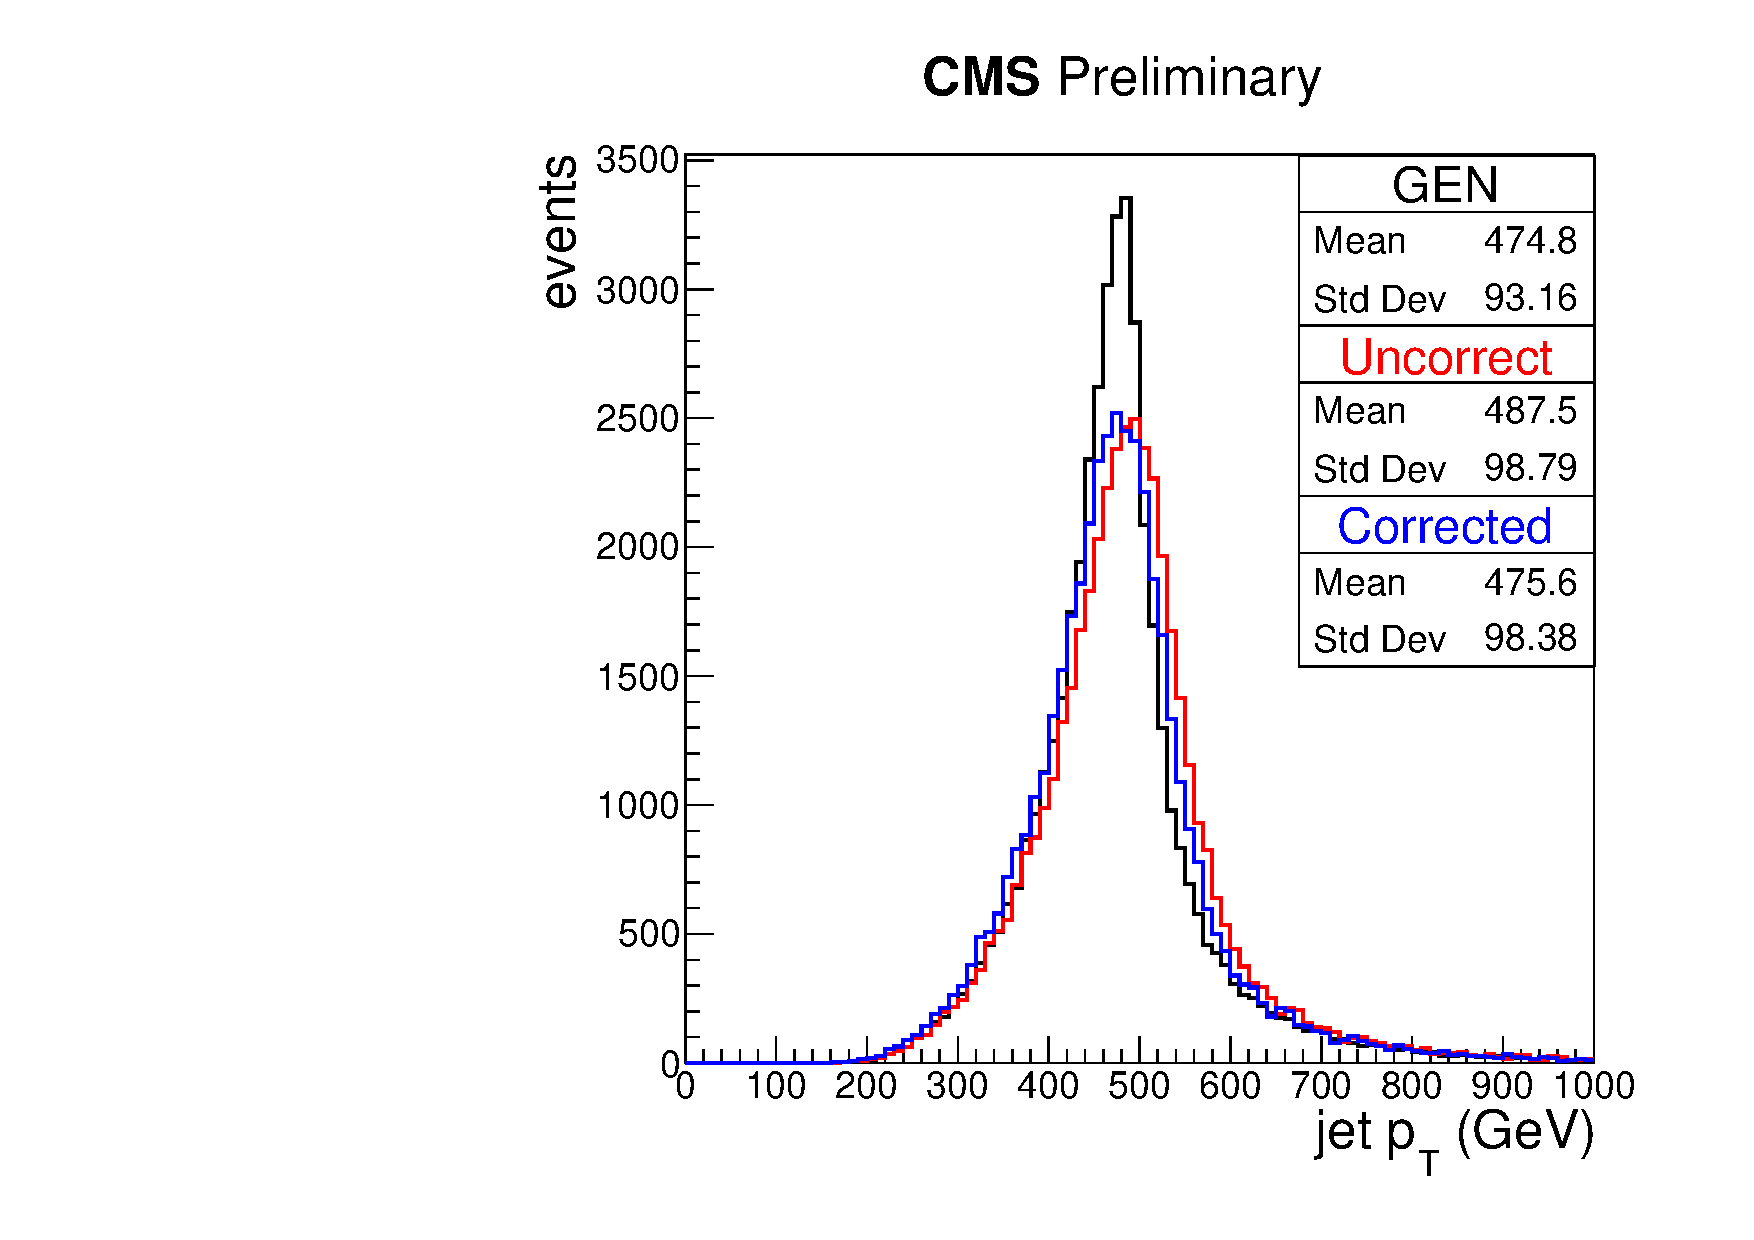
\includegraphics[width=0.47\textwidth]{figures/objects/corrJetPt.pdf}
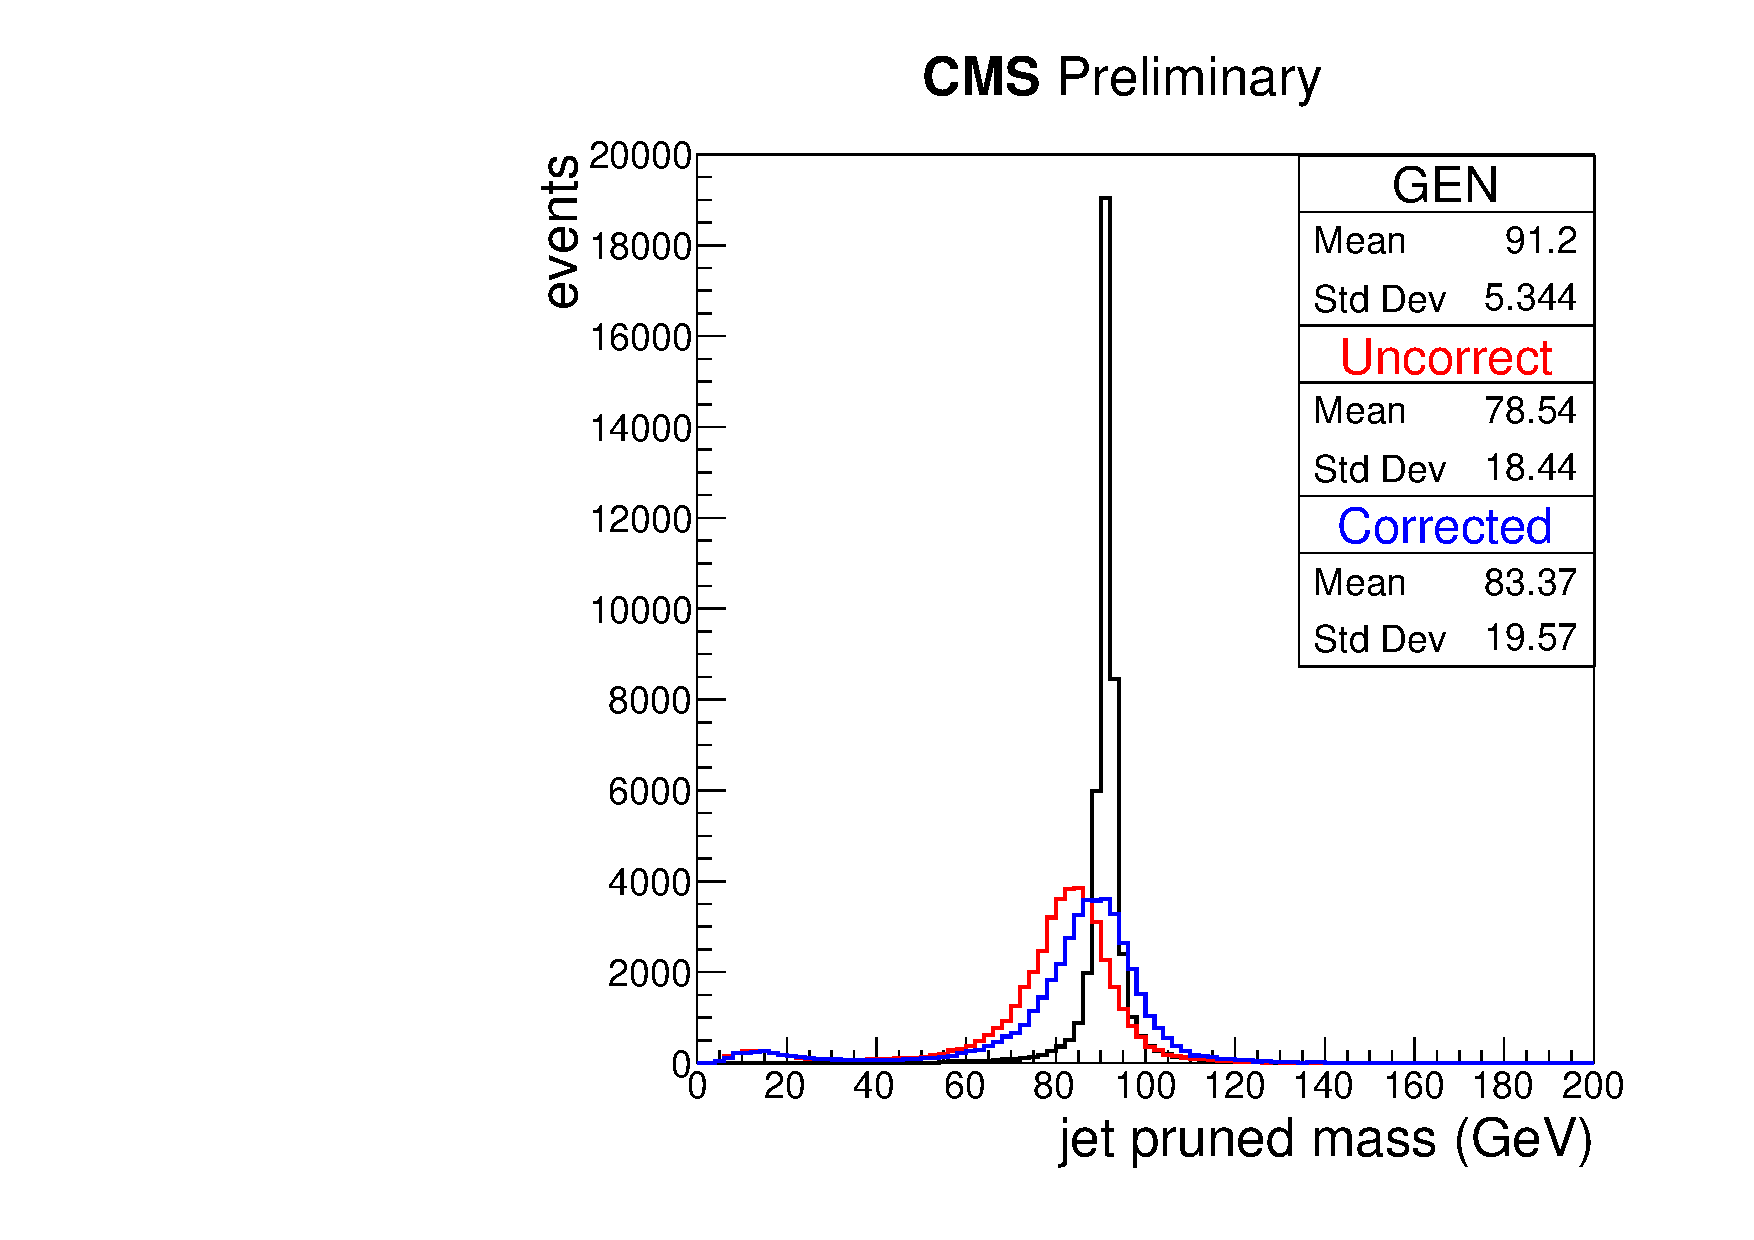
\includegraphics[width=0.47\textwidth]{figures/objects/corrPrunedMass.pdf}
\caption[Signal characterization]{Jet $p_{\rm T}$ (left) and jet mass (right) corresponding to a bulk graviton of mass 1 TeV. Jet energy corrections improve the agreement between the reconstructed jet and the generated Z boson.}
\label{signal1TeV}
\end{figure}

Other systematic uncertainties influence both the normalisation and shape of the background and signal. We consider effects from leptons (trigger, selection), hadrons (jet energy, V tagging), and LHC luminosity \cite{CMS-PAS-LUM-15-001}. Following the recommendations from the jet physics object group \cite{jetmetPOG}, we assign a relative uncertainty of 6.7\% (26\%) on the signal yield due to the V tagging in the high (low) purity category. Jet energy corrections (JEC) are considered to scale up/down the jet $p_{\rm T}$ affecting the position of the signal peak, as shown in Fig.~\ref{fig:jecUnc}. The associated systematic uncertainty due to the shift of the signal peak varies between 0.6\% and 0.95\%, and increases with the mass of the resonance. 

Lepton selections, both at trigger level and offline, also contribute to the systematic uncertainties. To estimate this uncertainty we vary the data/MC scale factors in each $\eta-p_{\rm T}$ bin, leading to the results shown in Fig.~\ref{fig:leptonUnc}. In summary, the systematic uncertainties taken into account are gathered in Table \ref{tab:systematics}.

\begin{table}[h!]
\begin{center}
\caption[Systematic Uncertainties]{Summary of systematic uncertainties on the signal normalization.}
\label{tab:systematics}
\begin{tabular}{lcl}
\hline\\[-0.2cm]
\textbf{Source}     & \textbf{Value} & \textbf{Comment} \\[0.2cm]
\hline\hline\\[-0.2cm]
Luminosity      & 2.7\%           & correlated between all categories \\[0.2cm]\hline\\[-0.2cm]
Electron trigger and ID & 2.5\% & tag-and-probe study \\[0.2cm] 
Electron energy scale   & 0.5\% & \\[0.2cm]\hline\\[-0.2cm]
Muon trigger and ID & 10\% & tag-and-probe study \\[0.2cm]
Muon momentum scale & 0.5\% & \\[0.2cm]\hline\\[-0.2cm]
Jet energy scale    & 1\% & correlated between all categories \\[0.2cm]\hline\\[-0.2cm]
V tagging           & 6.7\% & high purity \\[0.2cm]
                    & 26\%  & low purity  \\[0.2cm]
\hline
\end{tabular}
\end{center}
\end{table}

\begin{figure}[hb!]
\begin{center}
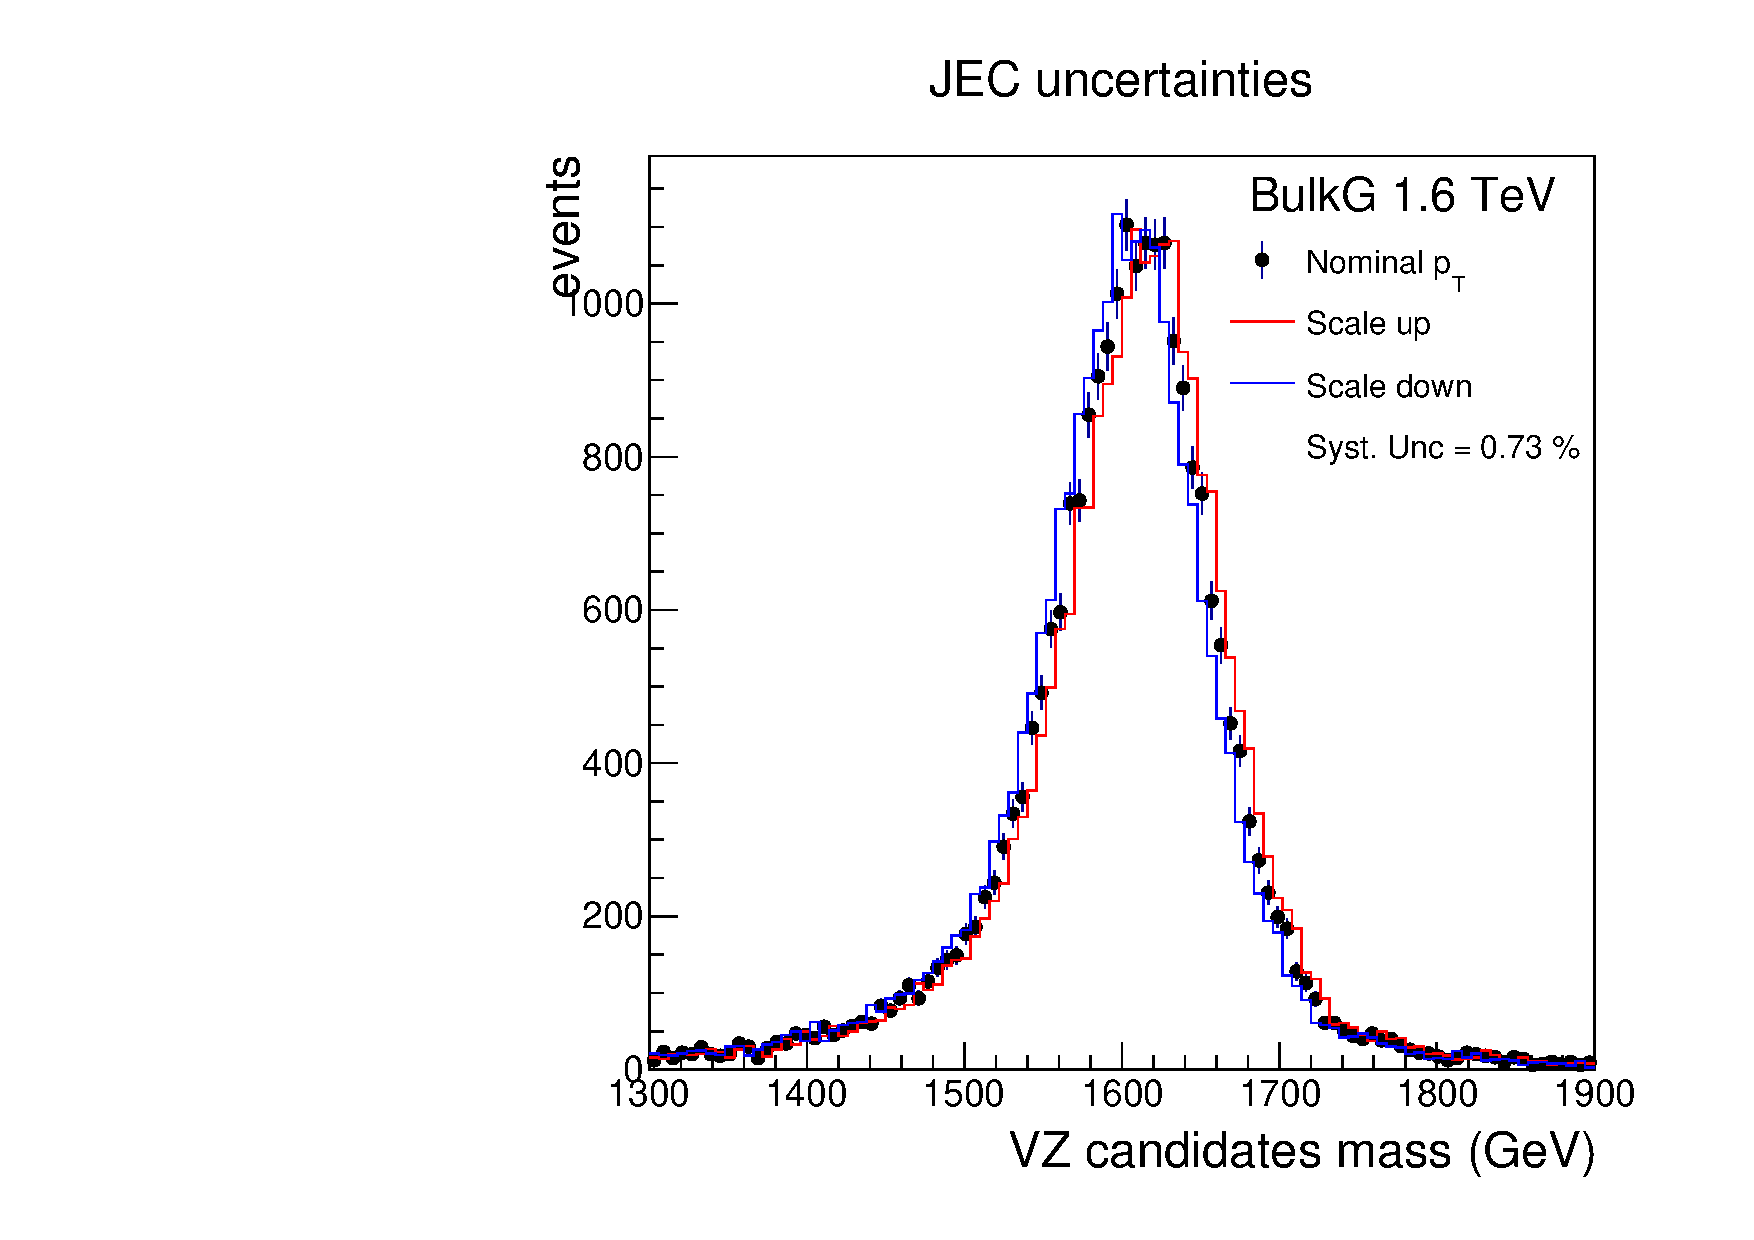
\includegraphics[width=0.47\textwidth]{figures/systematics/jecUnc1600.pdf}
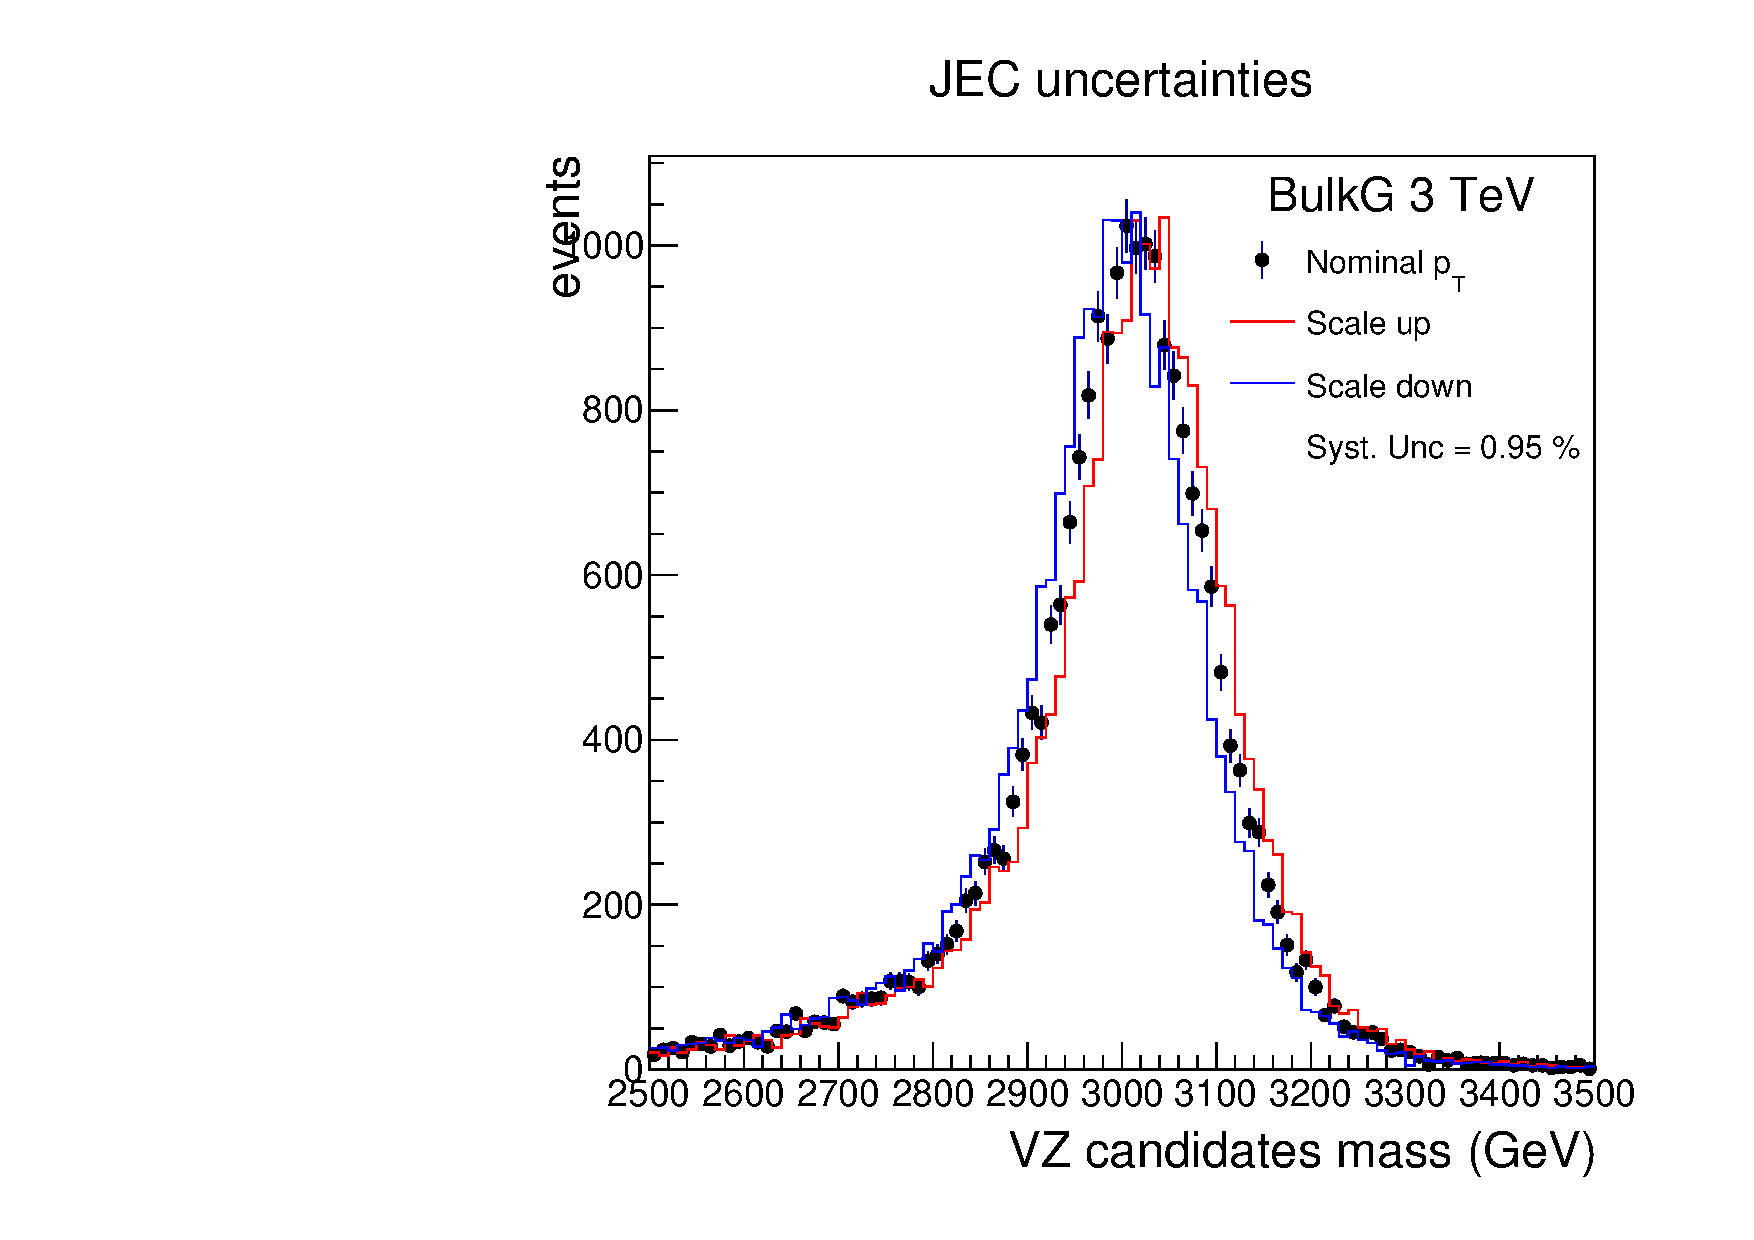
\includegraphics[width=0.47\textwidth]{figures/systematics/jecUnc3000.pdf}
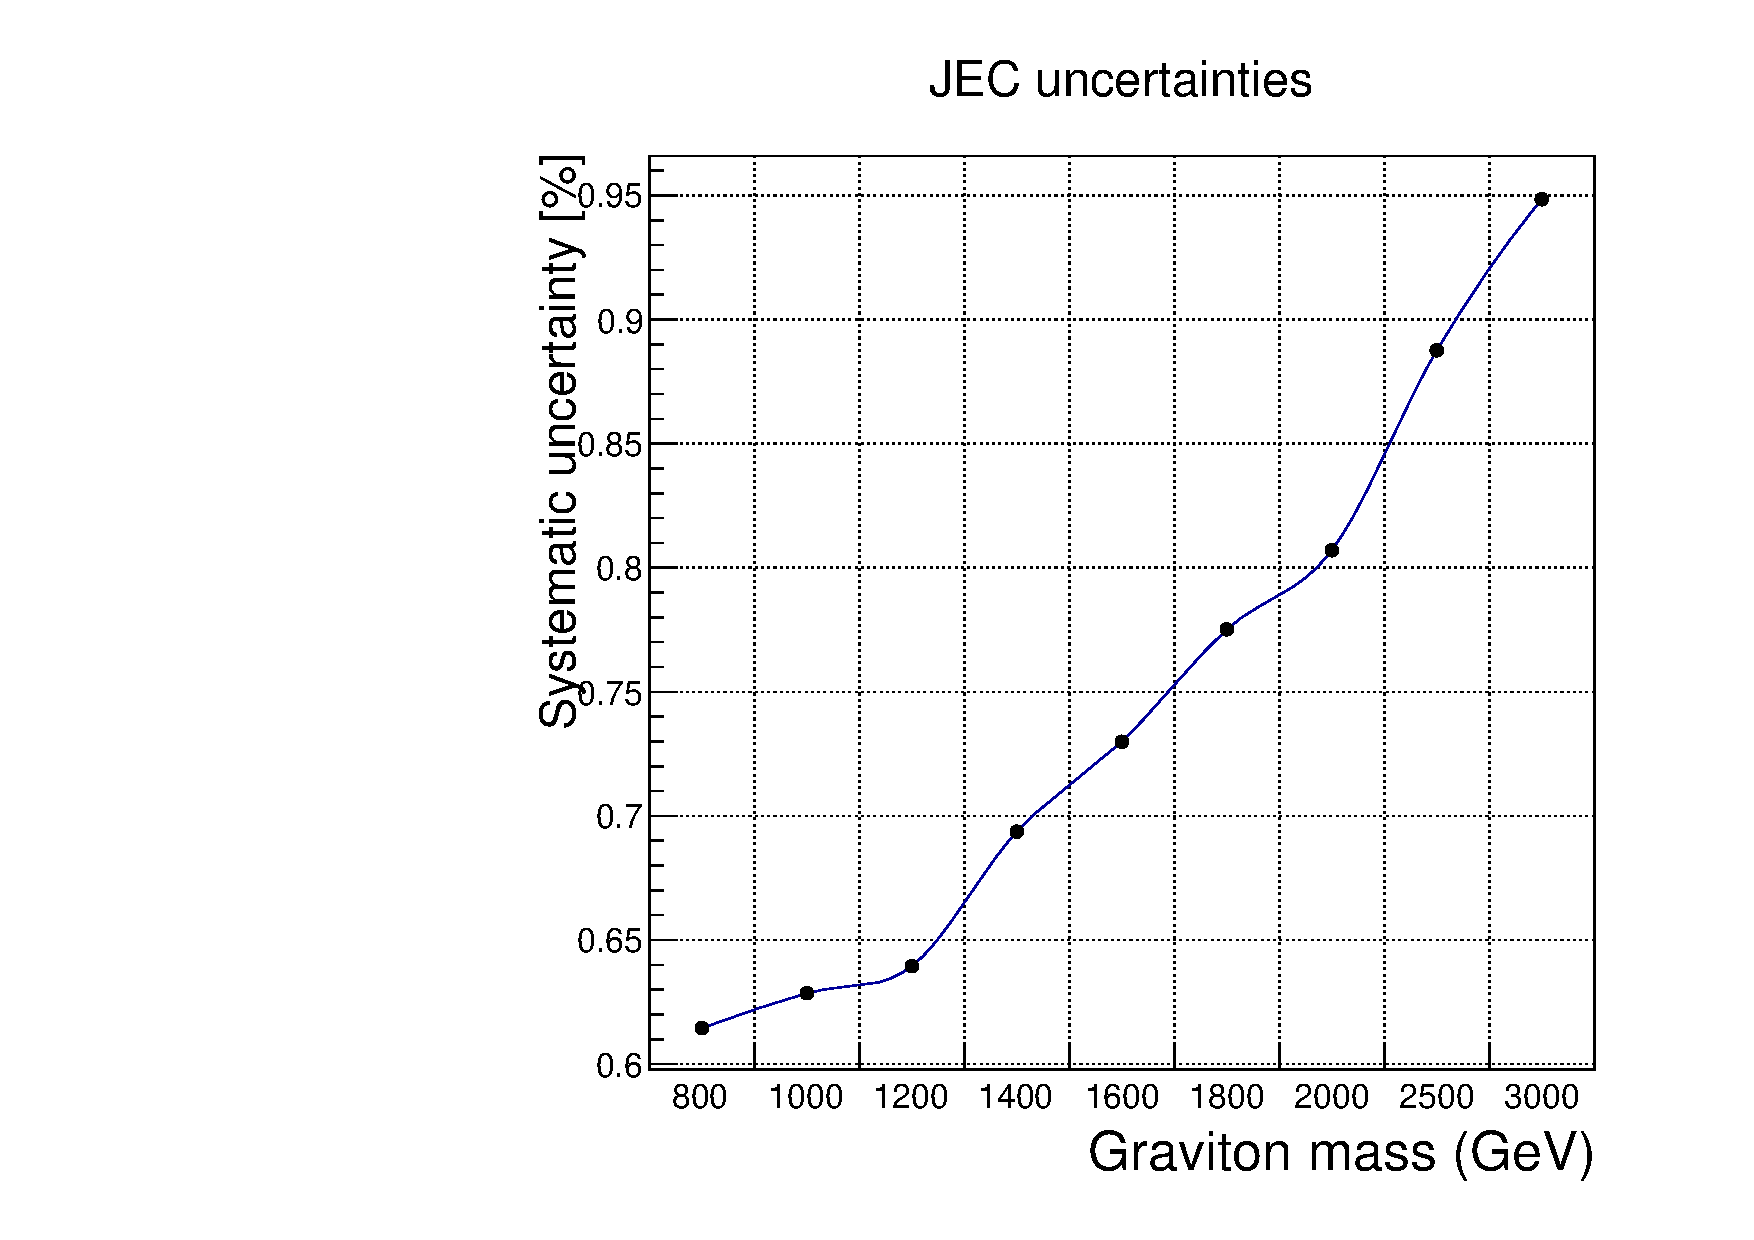
\includegraphics[width=0.47\textwidth]{figures/systematics/jecUncMean.pdf}
\caption[Uncertainties due to jet energy correction]{Scale up/down variations of jet energy correction (JEC) uncertainties, for a bulk graviton of mass 1.6 TeV (top-left) and 3 TeV (top-right). The associated systematic uncertainty due to the shift of the signal peak varies between 0.6\% and 0.95\% (bottom plot). }
\label{fig:jecUnc}
\end{center}
\end{figure}

\begin{figure}[h]
\begin{center}
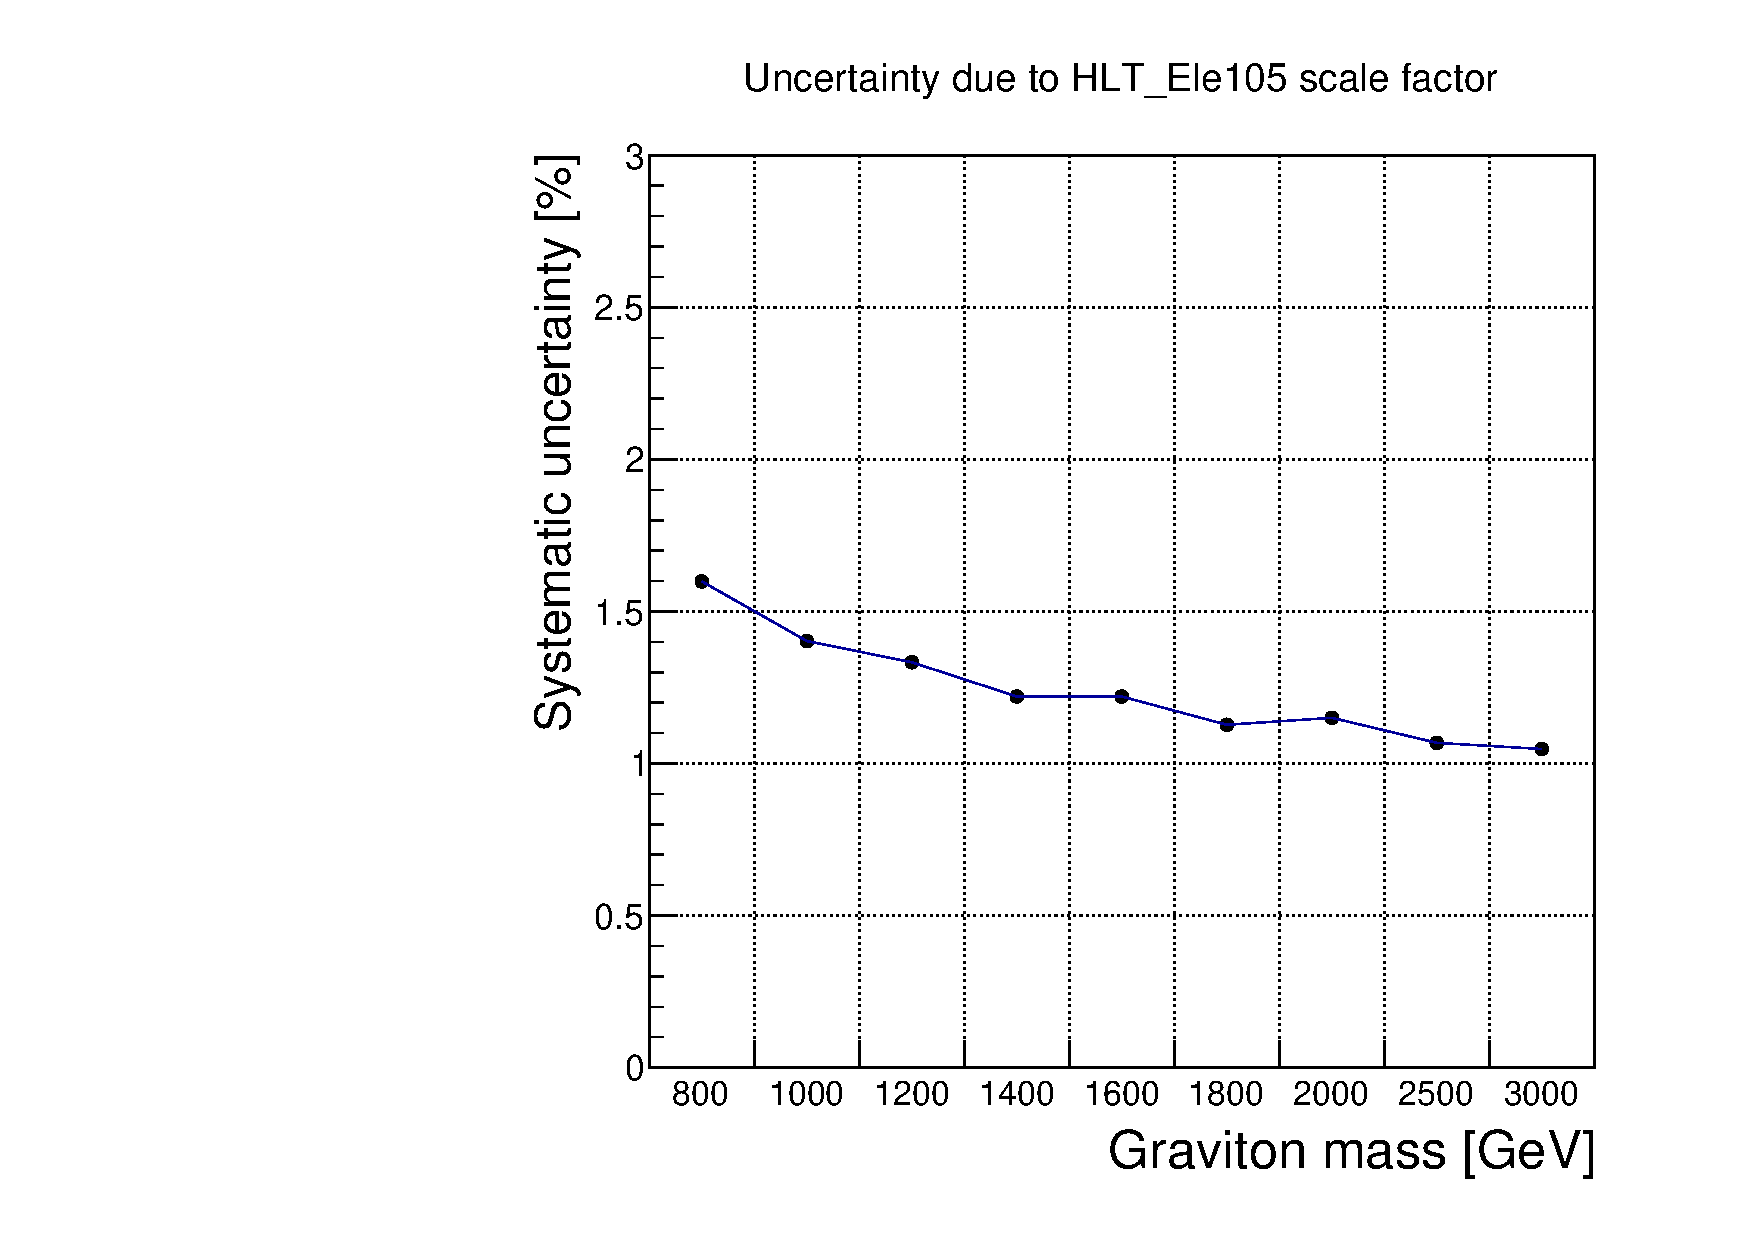
\includegraphics[width=0.47\textwidth]{figures/systematics/hltEleSFunc.pdf}
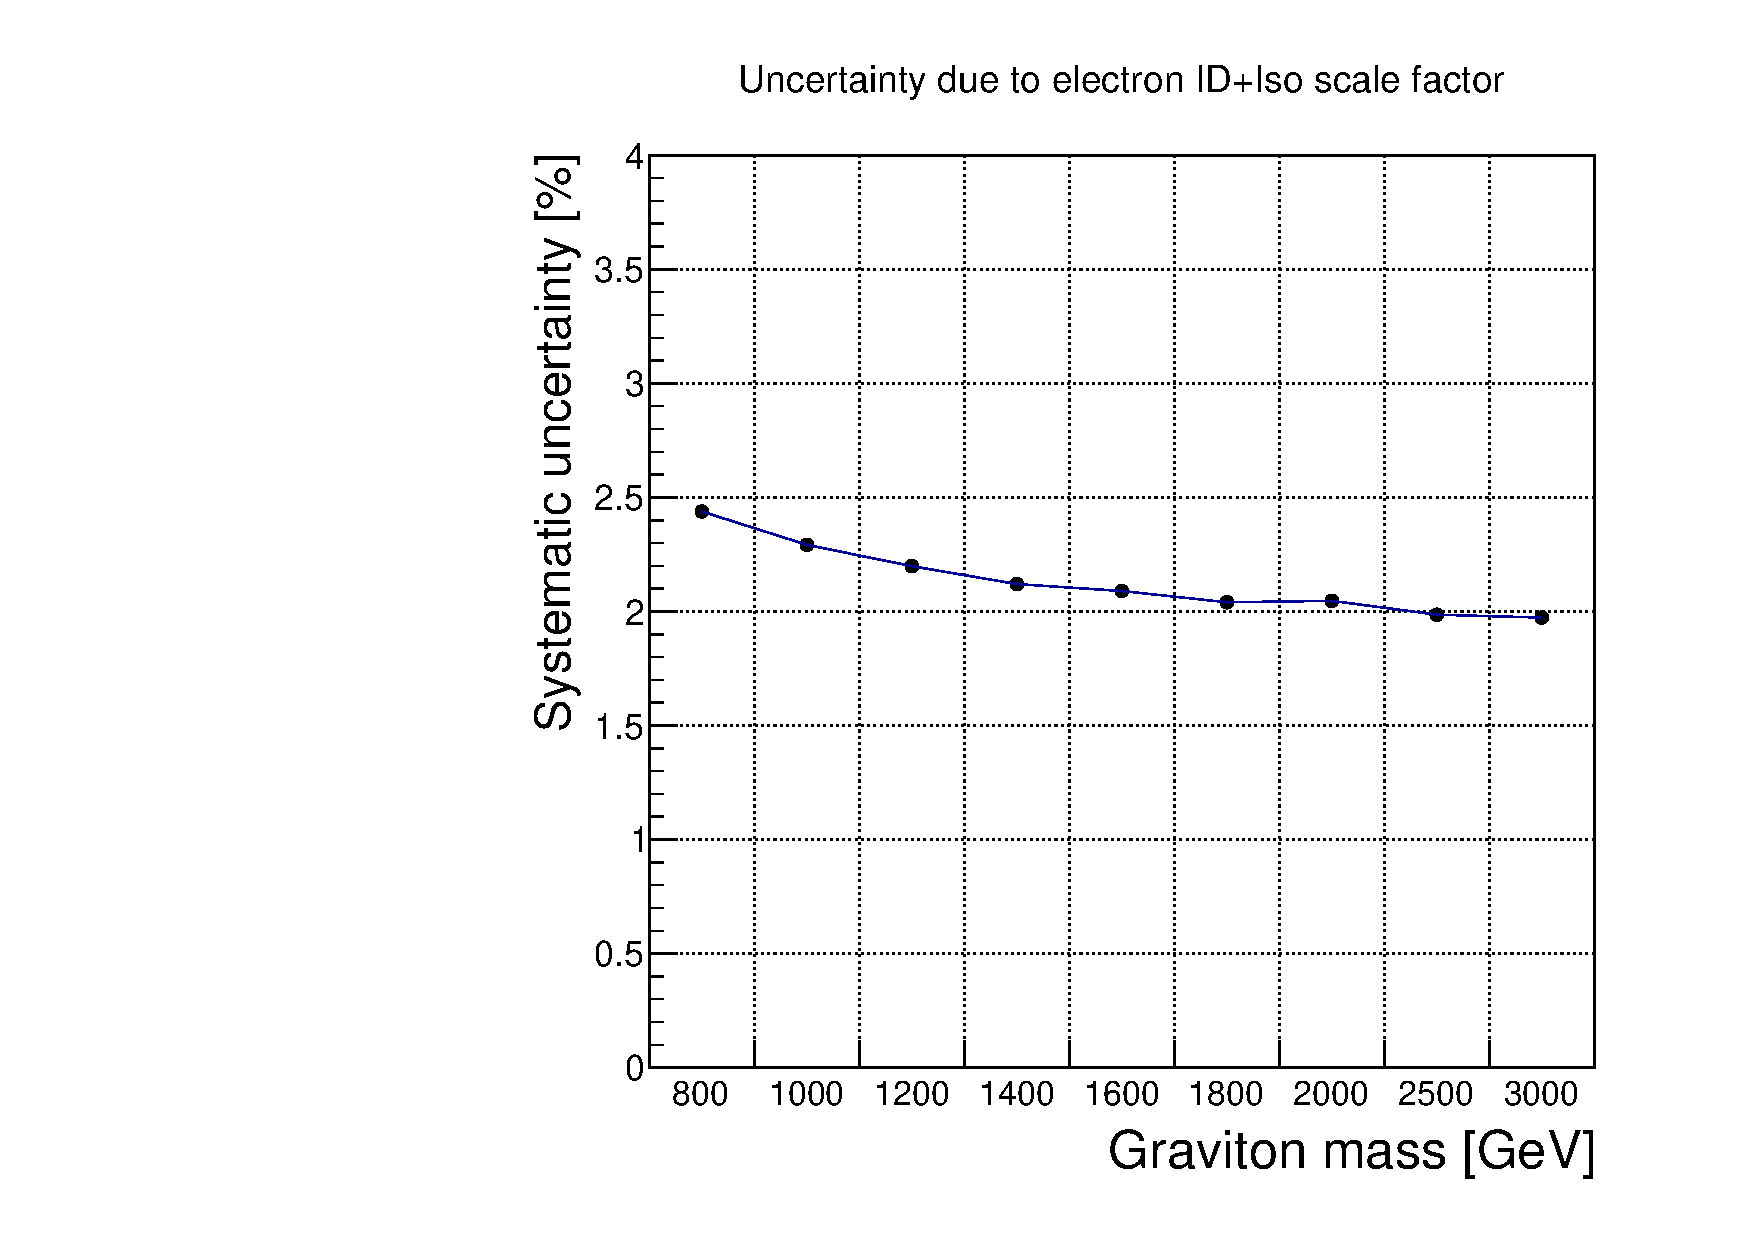
\includegraphics[width=0.47\textwidth]{figures/systematics/IDIsoEleSFunc.pdf}\\
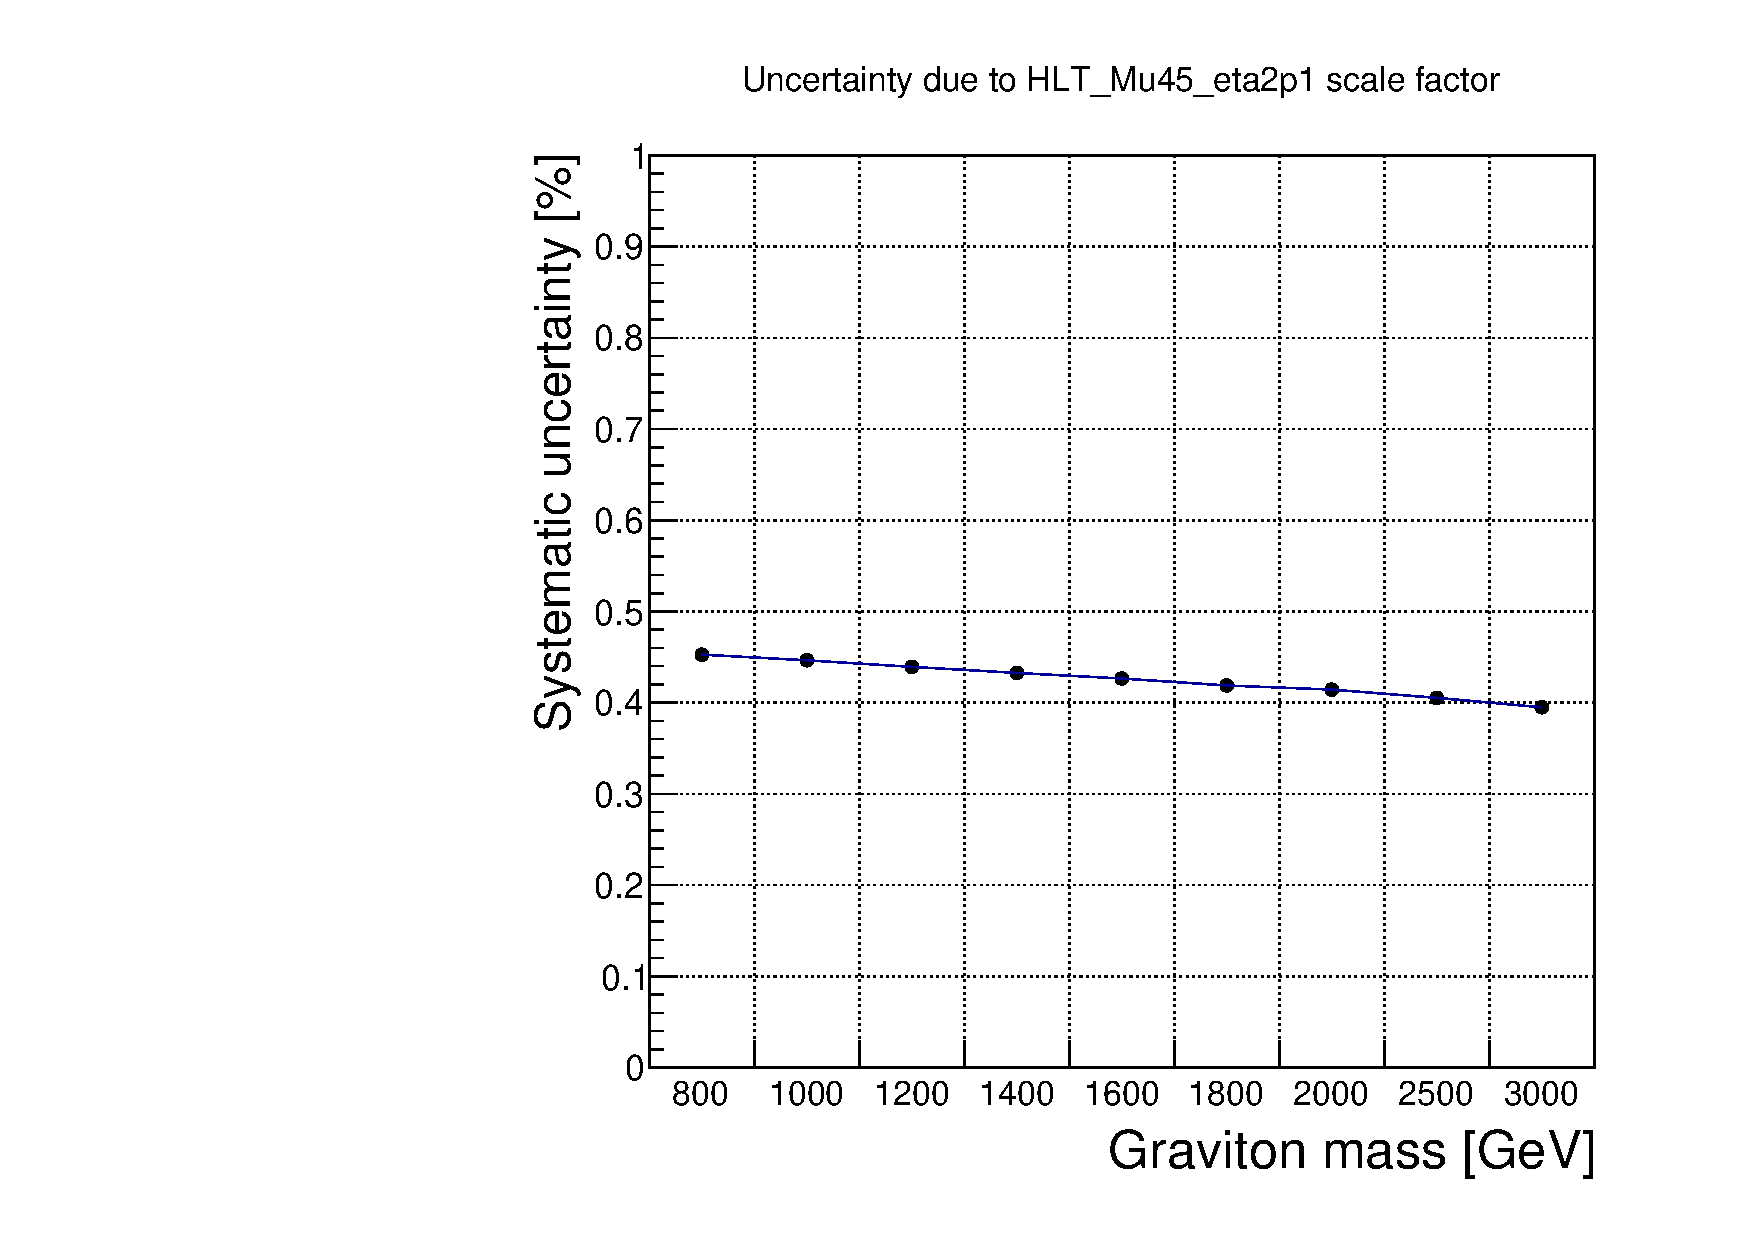
\includegraphics[width=0.47\textwidth]{figures/systematics/hltMuSFunc.pdf}
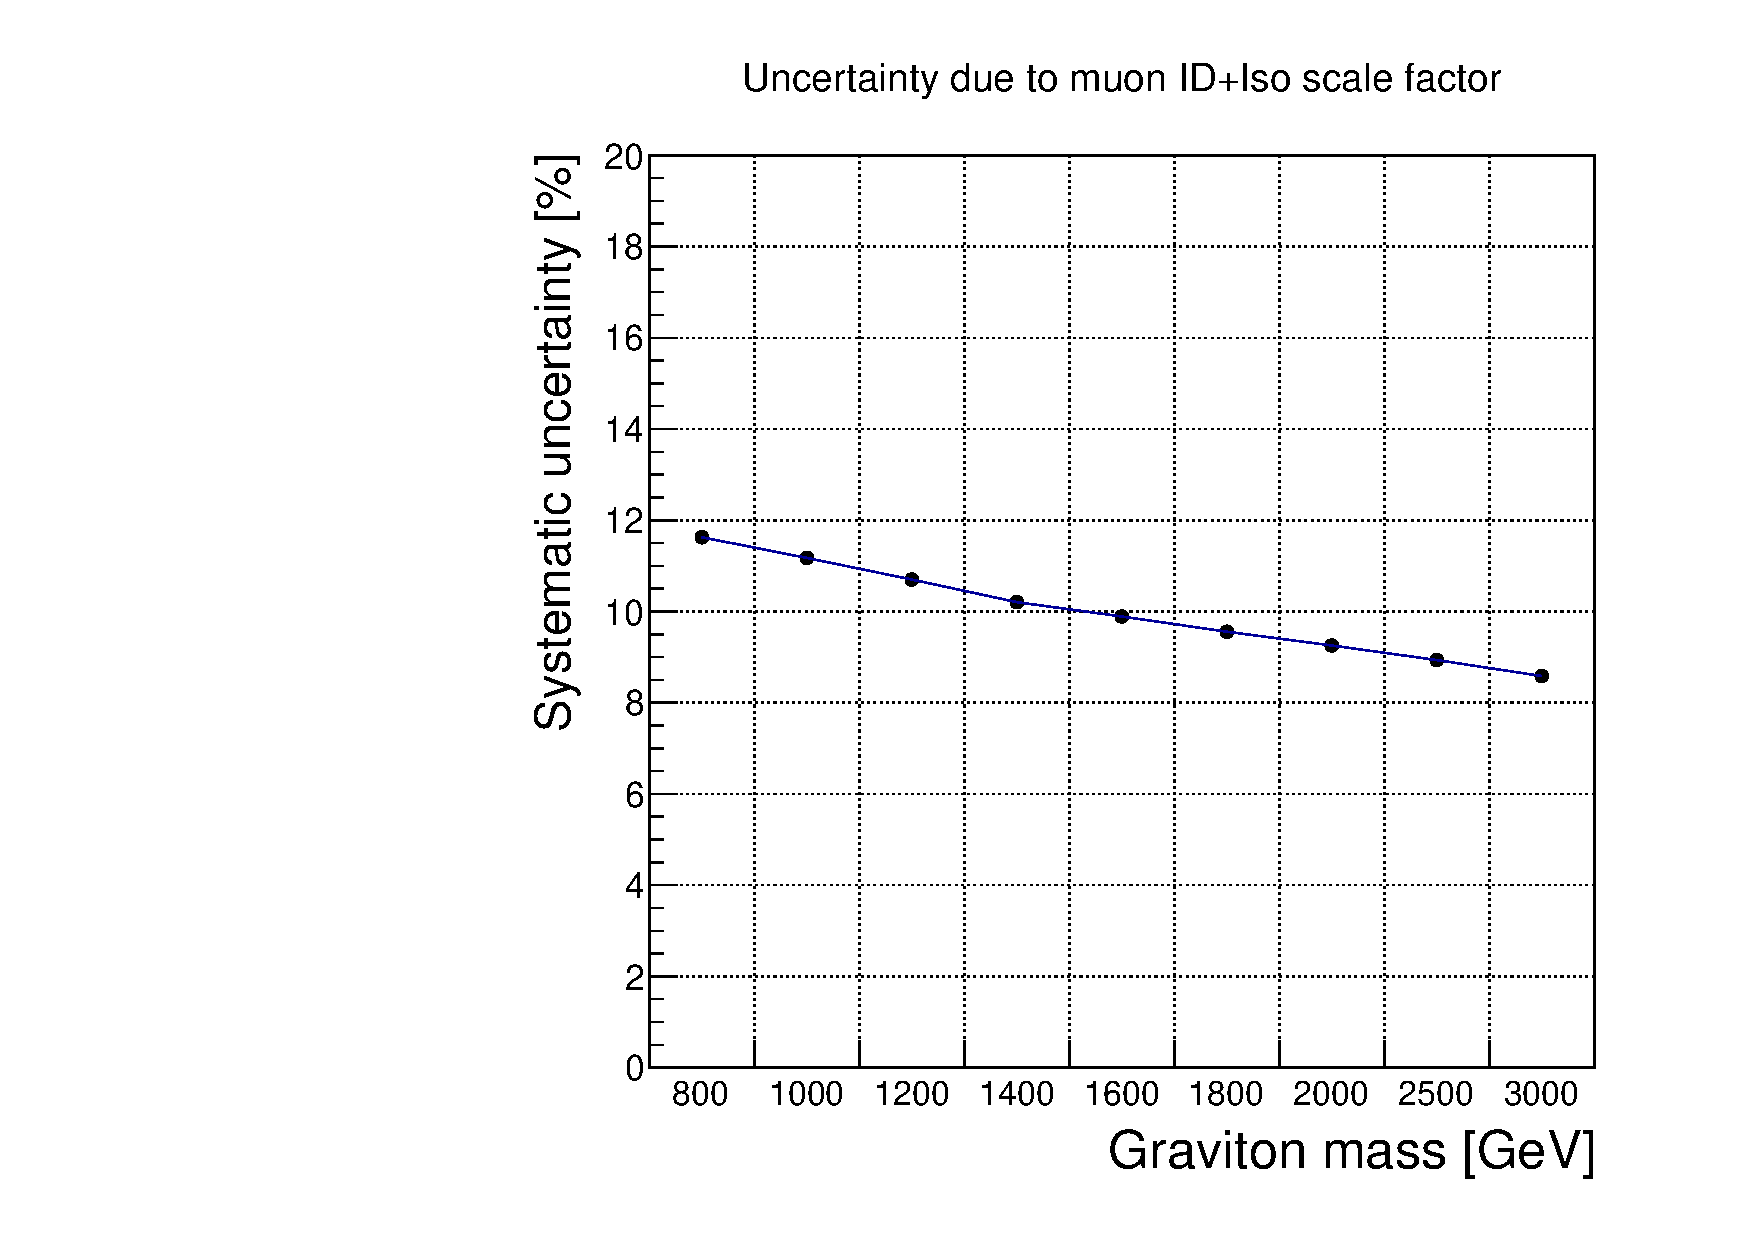
\includegraphics[width=0.47\textwidth]{figures/systematics/IDIsoMuSFunc.pdf}\\
\caption[Uncertainties due to lepton selection]{Systematic uncertainty due to the scale factors on the electron trigger (top-left), ID+Isolation (top-right). Systematic uncertainty due to the scale factors on the muon trigger (bottom-left), ID+Isolation (bottom-right).}
\label{fig:leptonUnc}
\end{center}
\end{figure}
